%% LyX 2.3.6 created this file.  For more info, see http://www.lyx.org/.
%% Do not edit unless you really know what you are doing.
\documentclass[12pt]{amsbook}
\usepackage{amstext}
\usepackage{xurl} 
\usepackage{amsthm}
\usepackage{newtxmath}
\usepackage{verbatim}
\usepackage[T1]{fontenc}
\usepackage[utf8]{inputenc}
\usepackage{geometry}
\geometry{verbose,tmargin=3cm,bmargin=3cm,lmargin=2.5cm,rmargin=2.5cm}
%\synctex=1
\usepackage{color}
\usepackage{verbatim}
\usepackage{prettyref}
\usepackage{float}
\usepackage{mathtools}
%\usepackage{makeidx}
\usepackage{nomencl}
\makenomenclature

\makeindex

\usepackage{graphicx}
\usepackage{xargs}[2008/03/08]

% the following is useful when we have the old nomencl.sty package
%\providecommand{\printnomenclature}{\printglossary}
%\providecommand{\makenomenclature}{\makeglossary}

\usepackage[unicode=true]
 {hyperref}

\usepackage{enumitem}
\setlist[enumerate,2]{label=\alph*)} % First level: lower-case letters (a, b, c, ...)
\setlist[enumerate,3]{label=\roman*)} % Second level: lower-case Roman numerals (i, ii, iii, ...)
\setlist[enumerate,1]{label=\arabic*)} % Third level: numbers (1, 2, 3, ...)


\makeatletter

%%%%%%%%%%%%%%%%%%%%%%%%%%%%%% LyX specific LaTeX commands.
%% Because html converters don't know tabularnewline
\providecommand{\tabularnewline}{\\}

\usepackage{cleveref}

\makeatletter
\newcommand{\myref}[2][]{%
	\def\@tempa{#1}%
	\ifx\@tempa\@empty%
	\hyperref[#2]{\ref*{#2}}%
	\else%
	\hyperref[#2]{#1 \ref*{#2}}%
	\fi%
}
\makeatother

%%%%%%%%%%%%%%%%%%%%%%%%%%%%%% Textclass specific LaTeX commands.
\numberwithin{section}{chapter}
\numberwithin{equation}{section}
\numberwithin{figure}{section}

% Define a new theorem style with bold title and no indentation
\newtheoremstyle{boldtheorem}
{}   % Space above
{}   % Space below
{\itshape} % Body font
{}          % Indent amount (set to 0)
{\bfseries} % Theorem head font
{.}         % Punctuation after theorem head
{.5em}      % Space after theorem head
{}          % Theorem head spec (can be left empty, meaning 'normal')

% Define theorem environment using the new style

\theoremstyle{boldtheorem}
\newtheorem{thm}{\protect\theoremname}
\theoremstyle{boldtheorem}
\newtheorem{cor}[thm]{\protect\corollaryname}
\theoremstyle{definition}
\newtheorem{defn}[thm]{\protect\definitionname}
\theoremstyle{remark}
\newtheorem{rem}[thm]{\protect\remarkname}
\theoremstyle{boldtheorem}
\newtheorem{lem}[thm]{\protect\lemmaname}
\theoremstyle{boldtheorem}
\newtheorem{prop}[thm]{\protect\propositionname}
\theoremstyle{definition}
\newtheorem{example}[thm]{\protect\examplename}
\theoremstyle{boldtheorem}
\newtheorem{conjecture}[thm]{\protect\conjecturename}

\usepackage{csquotes}
\usepackage[english,spanish,catalan]{babel}

\usepackage[
backend=bibtex,
giveninits=true,
backref=true,
hyperref=true, 
block=none,
]{biblatex}



\addbibresource{Biblatex-Tesis.bib}
%\addbibresource{/home/raul/Dropbox/Doctorado/Lyx/Auxiliares-Lyx/Biblatex-Doctorado.bib}

\usepackage{xcolor}
\definecolor{myorange}{RGB}{250,140,40}
\definecolor{mygreen}{RGB}{0,204,102}
\definecolor{mytitle}{RGB}{0,142,255}

%\definecolor{myorange}{RGB}{250,140,40}
%\definecolor{mygreen}{RGB}{40, 250, 140}
%\definecolor{myblue}{RGB}{140, 40, 250}
%\definecolor{myviolet}{RGB}{245,40,250}


\hypersetup{
	colorlinks=true, % false: boxed links; true: colored links
	linkcolor=myorange, % color of internal links
	citecolor=mygreen, % color of links to bibliography
	urlcolor=blue % color of external links
}

\DefineBibliographyStrings{english}{%
	backrefpage  = {\lowercase{s}ee p.}, % for single page number
	backrefpages = {\lowercase{s}ee pp.} % for multiple page numbers
}
\DeclareFieldFormat{postnote}{#1}



%\DeclareFieldFormat[article]{title}{\href{\thefield{url}}{#1}}
\DeclareFieldFormat[article]{title}{\textcolor{black}{#1}}
%\DeclareFieldFormat[article]{url}{}
% Redefine the bibliography driver to suppress certain fields
\AtEveryBibitem{
	\clearfield{doi} % Suppress DOI
	\clearfield{issn} % Suppress ISSN	
	\clearfield{eprint} % Suppress ISSN
}


% Define a custom bibliography driver
%\DeclareBibliographyDriver{article}{%	
%\printnames{author}%			
%\newunit\newblock	
%\iffieldundef{url}	
%{}
%{\href{\thefield{url}}{\printfield{title}}}%	
%\newunit	
%\printfield{journaltitle}%	
%\newunit	
%\printfield{year}%	
%\newunit	
%\printfield{pages}%	
%\finentry
%}



\makeatother


\def\eqdeclaration#1{, see equation\nobreakspace(#1)}
\def\pagedeclaration#1{, page\nobreakspace#1}
\def\nomname{Nomenclature}
\providecommand{\theoremname}{Theorem}
\providecommand{\conjecturename}{Conjecture}
\providecommand{\corollaryname}{Corollary}
\providecommand{\definitionname}{Definition}
\providecommand{\examplename}{Example}
\providecommand{\lemmaname}{Lemma}
\providecommand{\propositionname}{Proposition}
\providecommand{\remarkname}{Remark}



\makenomenclature
\begin{document}
\title{Garside Groups And The Yang-Baxter Equation}
\author{Author:\\
Raúl Sastriques Guardiola\\
\textcompwordmark\\
}
\author{PhD Advisors:\\
Adolfo Ballester Bolinches,\\
 José Sergio Camp Mora\\
\textcompwordmark\\
\textcompwordmark
\includegraphics[width=5cm]{logo_UV}\textcompwordmark\\
\textcompwordmark\\
Programa de Doctorado en Matématicas\\
Enero 2024}

\maketitle
\newcommandx\variables[3][usedefault, addprefix=\global, 1=x, 2=n, 3={,}]{#1_{1}#3#1_{2}#3...#3#1_{#2}}%

\selectlanguage{spanish}%

\chapter*{Agradecimientos}

Esta tesis doctoral es el resultado de estos últimos años de trabajo
y solo ha sido posible a muchas personas a las cuales quiero agradecer
aquí. 

En primer lugar, quiero agradecer a mis directores de tesis Adolfo
Ballester Bolinches por la confianza que me brindó al aceptar dirigir
esta tesis, dirección y labor administrativa, así como a José Sergio
Camp Mora por todo el tiempo y dedicación invertidos a lo largo de
la tesis doctoral.

Quiero agradecer también agradecer a mis padres, por el tiempo y paciencia
invertidos durante todos estos años, así como a mi familia más amplia,
por su apoyo, comprensión y cariño. 

Además, quiero agradecer y recordar, a todas aquellas personas con
las que me he encontrado en el camino, como el profesor Ramón Esteban
o mis compañeros del departamento de Álgebra; a Leandro Vendramin
por acogerme en Bruselas durante mi mes de estancia y por la magnifica
compañía de la cual pude disfrutar lejos de casa; a mis compañeros
de carrera y amigos Roberto Giménez, Irene Creus, Gabriel Calvo y
Paula Segura, por su amistad, templanza y por aquello vivido juntos. Por último quiero agradecer a aquellos, que si ser su obligación
me prestaron su ayuda como los profesores del Máster en Matemática
Avanzada de la UMU, y en particular, a Juan Jacobo Simón Pinero.

\chapter*{Resumen}

En 1998 Patrick Dehornoy y Luis Paris introdujeron en \cite{dehornoy99gaussian_and_garside}
la noción de grupos Garside, como una generalización de los grupos
Artin-Tits de tipo esférico, o tipo Coxeter finito. Desde entonces,
muchos autores han desarrollado la teoría de dichos grupos, tanto
sus propiedades computacionales (\cite{lee06abelian,lee11periodic,lee11translation,FRANCO2003112,sibert2004tame,doi:10.1081/AGB-100001665}...)
así como propiedades más abstractas (\cite{PICANTIN200192,picantin2013tree,chouraqui_garside_2010,godelle2013pregarside,godelle07parabolic,Dehornoy2015}....).
Hoy en día, la teoría de Garside todavía está en desarrollo, de hecho,
se podría decir que todavía está en sus primeros días de desarrollo.
Los grupos Garside no se han clasificado en diferentes familias de
manera completa, y como veremos, algunas familias de grupos Garside
están lejos de ser completamente entendidas, de hecho, carecen de
una clasificación/descripción adecuada en términos de grupos. Además,
existen numerosas generalizaciones de los grupos de Garside en la
literatura: pre-Garside \cite{godelle2013pregarside}, sistemas cuasi-Garside
\cite{godelle07parabolic}, gérmenes de Garside \cite{DEHORNOY2013109},
$l$-grupos a derecha \cite{rump2015right}. Sin embargo, en esta
tesis no desarrollaremos ninguna de estas generalizaciones sino que
usaremos la definición clásica de grupos de Garside introducida por
P. Dehornoy y L. Paris, aunque expresada en otros términos, para más
tarde, centrarnos en el estudio de una familia de Grupos de Garside
en particular: la familia de las soluciones conjuntistas finitas,
no degeneradas i involutivas de la ecuación de Yang-Baxter.

En el \myref[capítulo]{chap:Introduction-to-Garside} de la presente
tesis, veremos los conceptos básicos y necesarios sobre los grupos
de Garside para el desarrollo de nuestros nuevos resultados acerca
de este tema. 

Empezaremos en la primera sección con una discusión histórica acerca
de los grupos de Garside, esto es, qué los motivó, exponiendo brevemente
los grupos de trenzas y los grupos de Artin-Tits de tipo esférico,
los cuales constituyen los primeros ejemplos de grupos de Garside,
y que a su vez, suscitan un gran interés académico. En la siguiente
sección, veremos la definición formal de monoide de Garside así como
algunas de las propiedades básicas acerca de dichos monoides. Aún
sin entrar en la definición rigurosa, la cual veremos más adelante,
tenemos que un monoide $M$ es de Garside si es un monoide Gaussiano
(cancelativo, atómico y la divisibilidad a izquierda y derecha forma
un retículo) y tiene un elemento de Garside $\Delta\in M$ (esto es,
el conjunto de divisores a izquierda y derecha de $\Delta$ coinciden,
es finito y genera el monoide $M$). Cabe destacar que, pese a la
artificialidad de dicha definición, son muchos los monoides que la
cumplen, así como infinitos los elementos de Garside para un monoide
de Garside $M$. Así pues, es fácil ver que tanto el mínimo común
múltiplo como el máximo común divisor entre dos elementos de Garside
es también de Garside, así como cualquier potencia de un elemento
de Garside es también de Garside. Sin embargo, como veremos en la
presente tesis, existe un (único) elemento de Garside mínimo, el máximo
común divisor de todos ellos, el cual es de especial relevancia, y
el cual denotaremos por $\delta$. Si $M$ es un monoide de Garside,
tenemos que $M$ satisface el criterio de Ore, por lo que es posible
definir el grupo de fracciones de $M$, al cual llamamos grupo de
Garside y solemos denotar por $G$. Por último, destacaremos en esta
breve introducción la estructura introducida por M. Picantin en \cite{PICANTIN200192}
denominada cuasi-centro del monoide, $QZ\left(M\right)$, el cual
es libre, abeliano y finitamente generado, cuyos elementos tienen
todos la propiedad de ser equilibrados, esto es, el conjunto de divisores
a izquierda y a derecha coinciden, como en el caso de los elementos
de Garside, los cuales pertenecen a dicha estructura. Gracias al cuasi-centro
podemos clasificar un monoide de Garside como indescomponible, si
su cuasi-centro es un monoide cíclico infinito (generado por el elemento
de Garside minimal $\delta$).

Antes de entrar en mayor profundidad, tras ver algunas propiedades
elementales en la sección segunda, veremos algunos ejemplos notables
en la tercera sección, para así dar pie al estudio de los submonoides
parabólicos y de Garside en siguiente sección. Cabe destacar, como
es frecuente en el estudio de cualquier estructura algebraica, los
monoides de Garside contenidos a su vez dentro de un monoide de Garside
son de especial interés. Sin embargo, dichos submonoides, de no guardar
una especial relación con el monoide en el cual se encuentran contenidos
pueden no facilitar ninguna información acerca de este último, razón
por la cual la definición de submonoides parabólicos resulta imprescindible
al tiempo que constituye una generalización de los subgrupos parabólicos
usados en el estudio de los grupos de Artin-Tits. Destacamos el hecho
de que la intersección de dos subgrupos parabólicos estándar es de
nuevo un subgrupo parabólico estándar, lo cual permite a su vez definir
la unión de dos subgrupos parabólico estándar a partir de la intersección
de todos los subgrupos parabólicos estándar que los contienen. Con
respecto a estos subgrupos parabólicos, esta aún por ver si las propiedades
de dichos subgrupos en el caso de grupos de Artin se pueden trasladar
en su totalidad a los grupos de Garside en general. Así mismo, dar
una descripción completa de dichos subgrupos, es todavía, una labor
pendiente de los investigadores de los grupos de Garside. 

En las secciones quinta y sexta, abordamos el producto Zappa-Szép
de monoides, una generalización del producto semidirecto el cual nos
permite expresar un monoide de Garside como producto de submonoides
de Garside ``más simples'', esto es, indescomponibles en el sentido
introducido pon M. Picantin. Los resultados de esta sección son un
compendio de algunos de los resultados de V. Gebhardt y S. Tawn en
\cite{Gebhardt2016}, los cuales demuestran la equivalencia entre
producto Zappa-Szép y el ``producto cruzado'' introducido por M.
Picantin por el cual es posible escribir todo monoide de Garside como
producto Zappa-Szép/producto de submonoides con cuasi-centro cíclico
infinito. De hecho, aun cuando los autores de dichos artículos no
lo mencionan, es fácil ver que el cuasi-centro de un monoide de Garside
es cíclico si y solamente si el centro del monoide es cíclico. Como
veremos más adelante, en el capítulo segundo, es posible descomponer
un monoide de Garside cómo producto Zappa-Szép de submonoides cuyos
elemento de Garside minimales forman una base para el cuasi-centro
del monoide.

En la penúltima sección veremos como construir nuevos monoides de
Garside a partir de dos monoides de Garside, esta vez, usando el producto
libre amalgamado en lugar del Zappa-Szép, siendo este otro método
para la construcción de ejemplos y familias de grupos de Garside.
Finalmente, en la última sección expondremos de forma breve algunas
de las buenas propiedades computacionales que exhiben los monoides
de Garside, no siendo la finalidad de esta tesis la construcción de
nuevos algoritmos, sin embargo, parece pues relevante tener en cuenta
la posibilidad que ofrecen los monoides con la vista en futuras aplicaciones,
como puede ser la criptografía, entre otras.

\textcompwordmark{}

En el  \myref[capítulo]{chap:On-Zappa-Sz=0000E9p-decompositions}, expondremos
%algunos de nuestros resultados sobre los monoides de Garside en términos
del producto Zappa-Szép. Entre estos resultados, cabe destacar nuestros
hallazgos relacionando la descomposición del grupo de Garside $G$
en términos Zappa-Szép, y factorización de los elementos de Garside
del grupo $G$ en términos de los elementos de Garside de los factores
Zappa-Szép.
\begin{thm}
Si $G$ es un monoide de Garside tal que $G=H\bowtie K$ y denotamos
por $\delta_{G},\delta_{H}$ y \textup{$\delta_{K}$} a los elementos
de Garside minimales de $G,H$ y $K$ respectivamente, entonces $\delta_{G}=\delta_{H}\delta_{K}$.
\end{thm}

De forma más general, tenemos:
\begin{thm}
Sea $G$ un monoide de Garside que descompone como el producto Zappa-Szép
de ciertos monoides de Garside indescomponibles $\variables[H]$.
Si $\delta_{G}$ denota el elemento de Garside minimal de $G$, entonces
$\delta_{G}=\variables[\delta][][\cdot]$ donde $\delta_{i}$ es el
elemento de Garside minimal de $H_{i}$ para $i=1,...,n$. Adicionalmente,
$\delta_{G}^{k}=\variables[\delta^{k}][n][\cdot]$ para todo $k\in\mathbb{Z}$. 
\end{thm}

Otro resultado a destacar es la descripción de todos los elementos
de Garside de un grupo de Garside. Cuando el grupo de Garside $G$
es indescomponible, entonces todo elemento de Garside es una potencia
positiva del elemento de Garside minimal de $G$. Para el caso descomponible,
tenemos lo siguiente:
\begin{thm}
Si $G$ es un monoide de Garside tal que $G=H\bowtie K$ con $H,K$
dos monoides de Garside indescomponible, entonces $\left\{ \delta_{H}^{a}\delta_{K}^{b}\mid a,b\geq1\right\} $
es el conjunto de todos los elementos de Garside de $G$.
\end{thm}

Motivados por el resultado anterior y teniendo por finalidad una descripción
detallada de los elementos de Garside de $G$, demostramos el resultado
siguiente:
\begin{thm}
Sea $G$ un monoide de Garside y sea $\left\{ \variables[x][r]\right\} $
una base del cuasi-centro de $G$. Si $A_{i}$ el es conjunto de átomos
dividiendo a $x_{i}$, y llamamos $N_{i}$ al submonoide generado
por $A_{i}$, entonces $G$ se descompone como el producto Zappa-Szép
de los monoides $N_{1},...,N_{r}$, de modo que $N_{i}N_{j}=N_{j}N_{i}$
dados $i,j\in\left\{ 1,...,r\right\} $, y tal que el producto Zappa-Szép
es asociativo.
\end{thm}

Así pues, somos capaces de expresar un grupo de Garside como producto
de subgrupos parabólicos cuyos elementos de Garside conmutan entre
sí formando una base para el cuasi-centro de $G$. Llamamos a los
términos $N_{1},...,N_{r}$ anteriores, factores cuasi-centrales de
$G$. Gracias al anterior resultado, tenemos ahora:
\begin{cor}
Sea $G$ un monoide de Garside, y sea $\variables[N][r]$ su descomposición
en términos cuasi-centrales. Si denotamos por $\delta_{N_{i}}$ al
elemento de Garside minimal de $N_{i}$ para $i=1,...,r$, entonces
$\left\{ \delta_{N_{1}}^{e_{1}}\cdot...\cdot\delta_{N_{r}}^{e_{r}}|e_{i}\geq1\text{ for }i=1,...,r\right\} $
es el conjunto de todos los elementos de Garside de $G$.
\end{cor}

Finalmente, destacaremos un último resultado del capítulo segundo,
el cual responde a la cuestión acerca de como podemos describir los
submonoides parabólicos en términos de una descomposición Zappa-Szép,
al tiempo que suscita la cuestión acerca de la relación que guardan
los factores de una descomposición con respecto a la totalidad de
los submonoides parabólicos.
\begin{thm}
Sea $G$ un monoide de Garside el cual admite una descomposición en
términos Zappa-Szép $\variables[M][r]$. Si $S$ es un submonoide
parabólico de $G$, entonces $S$ es el producto Zappa-Szép de los
submonoides $S_{i}=S\cap M_{i}$.
\end{thm}

En el  \myref[capítulo]{chap:Introduction-to-the}, cambiamos de manera
aparente el tema de estudio para centrarnos en la ecuación cuántica
de Yang-Baxter, la cual, bajo condiciones específicas, tal y como
veremos, nos provee de una familia de grupos de Garside, de gran interés
en la literatura académica.

Finalmente, remarcamos aquí que si bien todo lo expuesto en estos
dos capítulos posee una gran relevancia para el estudio de los grupos
de Garside, no todo aquello que posee una gran relevancia para dicho
estudio esta presente en estos capítulos. Así mismo, pese a resultar
posible el extenderse más en las cuestiones expuestas, resulta necesario
poner fin a dicho desarrollo aun cuando con ello se dejen de explorar
otras cuestiones. Así pues, quedan abiertas al estudio cuestiones
ya abiertas con anterioridad, tales como si la existencia de un plegamiento
fuerte de una solución implica necesariamente la descomponibilidad
de dicha solución (véase \cite{chouraqui_folding_2012}). Al mismo
tiempo, resulta de interés razonar bajo que condiciones el producto
de subgrupos parabólicos estándar sea de nuevo parabólico estándar,
así como qué relación guardan los factores principales con respecto
a este tipo de subgrupos. Otra cuestión sería si dichos subgrupos
parabólicos forman un retículo, al igual los divisores del elemento
de Garside $\Delta$. Por último, destacamos que dichos subgrupos
en el caso de Artin-Tits han sido extensamente estudiados, razón por
la cual resulta de interés saber qué propiedades de dichos grupos
son generalizables al caso de Garside en general y cuáles son particulares
de dichos grupos.

\textcompwordmark{}

Con el propósito de estudiar una familia en concreto de grupos de
Garside, empezamos el capítulo tercero de esta tesis. Dicha familia
resulta de gran interés, más allá de la teoría de Garside, pues aparece
en el ámbito del estudio de la ecuación cuántica de Yang-Baxter (ECYB),
la cual ha suscitado un gran interés en el ámbito del álgebra en las
últimas dos décadas. Esta ecuación, con origen en la física teórica,
fue introducida por primera vez por C.N. Yang \cite{yang1967some}
y posteriormente en \cite{baxter19731} de R. Baxter. Una solución
de ECYB es un aplicación lineal $R:V\otimes V\longrightarrow V\otimes V$
donde $V$ es un espacio vectorial que satisface una ecuación particular:

\begin{equation}
R^{12}R^{13}R^{23}=R^{23}R^{13}R^{12},
\end{equation}
donde $R^{ij}:V\otimes V\otimes V\longrightarrow V\otimes V\otimes V$,
viene dada por $R$ en las componentes $i,j$ y actúa como la identidad
en la otra componente. El problema de construir y clasificar estas
soluciones sigue siendo un área activa de investigación. Si bien el
estudio del ECYB condujo a la fundación de grupos cuánticos en la
física matemática, el estudio de las soluciones no degeneradas i involutivas
se ha relacionado con muchas áreas matemáticas, tales como: álgebras
binomiales cuánticas \cite{gateva1994noetherian,gateva1996skew},
semigrupos de tipo $I$ y grupos de Bieberbach \cite{gateva1998semigroups,tate1996homological,jespers05groups_I_type},
coloraciones de curvas planas y 1-cociclos biyectivos \cite{Etingof98set_theoretical},
álgebras de Hopf triangulares, mínimas y semisimples \cite{etingof1998method},
sistemas dinámicos \cite{veselov2003yang}, cristales geométricos
\cite{etingof2003geometric}, llaves y anillos radicales \cite{rump_braces_2007,bachiller16thesis},
subgrupos regulares de las extensiones holomorfas y Hopf-Galois \cite{featherstonhaugh2012abelian,catino_colazzo_stefanelli_2015},
``racks'' y álgebras de Hopf \cite{eisermann2005yang,radford2011hopf,rump2022classification},
grupos trifactorizados (\cite{sysak2010products,fuster2021left}),
grupos Garside, gérmenes de Garside y $RC$ cálculos \cite{chouraqui_garside_2010},
y ``cycle sets'' \cite{rump2005square-free}, por el momento...

\textcompwordmark{}

En la primera sección de este capítulo, veremos la definición de solución
(conjuntista) de la ecuación de Yang-Baxter (EYB) siendo nuestro objeto
exclusivo de estudio dichas soluciones bajo las condiciones de ser
no degeneradas, involutivas y estar definidas sobre un conjunto finito.
Para este tipo de soluciones, las cuales denotamos mediante el par
$\left(X,S\right)$ con $X$ un conjunto finito y $S:X^{2}\rightarrow X^{2}$,
podemos definir otras estructuras algebraicas, tales como el grupo
de estructura de la solución:
\[
G\left(X,S\right)=\left\langle X\mid xy=tz\text{ dado }S\left(x,y\right)=\left(t,z\right)\right\rangle .
\]

Asimismo, dado que cada una de las componentes de $S$ define una
permutación de $X$, si escribimos $S(x,y)=\left(g_{x}(y),f_{y}(x)\right)$
para $x,y$ en $X$, entonces podemos definir el grupo de permutación
asociado a la solución $\left(X,S\right)$ como el subgrupo de $\text{Sym}_{\left|X\right|}$
generado por $\left\{ g_{x}\mid x\in X\right\} $. Además, existe
una permutación $T$ de $X$, tal que la identidad $f_{x}^{-1}T=Tg_{x}$
se cumple para todo $x\in X$. Así pues, el subgrupo generado por
$\left\{ f_{x}\mid x\in X\right\} $ es isomorfo al grupo de permutación
anteriormente definido. Dichos objetos matemáticos, fueron definidos
por primera vez por P. Etingof, A. Soloviev y T. Schedler en \cite{Etingof98set_theoretical},
en donde, entre otras cosas, se clasificaron y construyeron todas
las soluciones finitas, no degeneradas i involutivas de la EYB, definidas
sobre un conjunto $X$ con a lo sumo $8$ elementos. Así mismo, también
cabe destacar otras aportaciones realizadas por lo autores del artículo
anteriormente señalado a la clasificación y estudio de las soluciones,
en particular, los conceptos de solución retractable y multipermutacional.
Decimos que una solución $\left(X,S\right)$ es retractable cuando
$g_{x}=g_{y}$ para distintos $x,y\in X$. En tal caso, la relación
$x\sim y$ establece una relación binaria de equivalencia compatible
con $S$, tal que es posible definir una nueva solución sobre $X/\sim$,
denominada solución retractada de $\left(X,S\right)$. En los casos
en que es posible retractar una solución y su solución retractada,
reiteradamente hasta obtener la solución definida sobre un conjunto
con un solo elemento, llamamos a dicha solución multipermutacional.
Con estas nociones, entre otras, podemos entrar a desarrollar y profundizar
acerca de las soluciones de la EYB en la cuarta sección del capítulo. 

En la segunda sección, introducimos los grupos IYB y el concepto de
$I$-estructura, el cual nos permite describir el grupo de estructura
con mayor facilidad y claridad. Un grupo finito es un grupo IYB, si
es el grupo de permutaciones de una solución finita no degenerada
i involutiva de la EYB. En dicha sección exploramos algunos de los
resultados sobre la IYB ya conocidos, de los cuales destacamos el
hecho de que todo subgrupo de Hall de un grupo IYB es de nuevo un
grupo IYB, además, el producto directo de grupos IYB es de nuevo IYB
y todo grupo finito resoluble es isomorfo a un subgrupo de un grupo
IYB. Si bien existen métodos para la construcción de grupos IYB a
partir de otros grupos IYB, tan solo haremos referencia a los respectivos
artículos, dada la complejidad de dichos resultados.

En la tercera sección, introducimos de forma breve la estructura algebraica
conocida como Braza a izquierda, la cual también resulta de utilidad
por tal de estudiar dichas soluciones, aun cuando no desarrollaremos
nuestros resultados por esta vía, si bien nos resultará de utilidad
a la hora de exponer ciertos resultados. Dicho de forma gruesa, una
braza a izquierda, es el resultado de definir sobre el grupo de permutaciones
de una solución, una operación suma $+$, la cual proviene de considerar
la permutación asociada a un elemento $z$ del grupo de estructura
asociado a la solución. Por ello, a partir de la terna $\left(\mathcal{G},+,\cdot\right)$
que define la braza, tenemos una estructura que encapsula suficiente
información sobre la solución, como para resultar equivalente el estudio
de brazas a izquierda con el estudio de soluciones finitas, no degeneradas
e involutivas. Cabe destacar, que el concepto de braza a izquierda
es un elemento que ha sido generalizado a través de las brazas a izquierda
``retorcidas'' (``skew left braces'' en inglés), las cuales guardan
a su vez relación con soluciones de la EYB en condiciones más generales
de las señaladas con anterioridad. 

En la sección cuarta, encontramos un compendio acerca de los principales
resultados sobre las soluciones de la EYB para el caso de la presente
tesis, esto es: no degeneradas, finitas i involutivas. Así, por ejemplo,
sabemos que si $\left(X,S\right)$ es una solución finita, no degenerada
i involutiva, entonces es indescomponible si y solamente si el grupo
de permutaciones $\mathcal{G}$ actúa transitivamente sobre $X$.
Si $\mathcal{G}$ es abeliano, entonces la solución es retractable,
y si es cíclico, entonces es multipermutacional. Tal y como estos
resultados sugieren, existe una íntima relación entre propiedades
de los grupos asociados y propiedades de las soluciones de la EYB.
Dichos resultados suscitaron nuestro interés por incorporar técnicas
de teoría de grupos al estudio de la EYB. 

En la quinta sección, exponemos la relación entre las soluciones de
la EYB y los grupos de Garside. Tal y como probó F. Chouraqui en \cite{chouraqui_garside_2010},
todo grupo de estructura de una solución finita, no degenerada i involutiva,
es un grupo de Garside que satisfacen ciertas propiedades adicionales
(H), y recíprocamente todo grupo de Garside que satisfacen (H), es
el grupo de estructura de una solución finita no degenerada i involutiva.
Además, los conceptos de descomposición de una solución de la EYB
y la descomposición mediante el producto Zappa-Szép del grupo de Garside
resultan ser equivalentes. Consecuentemente, los grupos de Garside
que satisfacen (H) constituyen una familia cerrada para la descomposición,
sobre la cual disertaremos en lo restante de tesis. 

Finalmente, en la última sección exploramos una nueva vía para la
clasificación de los grupos de Garside relacionados con la EYB, haciendo
uso de los hallazgos de P. Dehornoy en \cite{dehornoy_coxeter_like_2013}
y \cite{dehornoy_set_theoretic_2015}. Tal y como el autor demostró,
si $G$ es el grupo de estructura de una solución finita, no degenerada
e involutiva de la EYB $\left(X,S\right)$, entonces existe un entero
positivo $d$, el cual llamamos clase de Dehornoy, tal que $G$ tiene
un cociente $W$ de orden $d^{\left|X\right|}$, el cual caracteriza
la solución. Además, dicho resultado es explicito, esto es, es posible
construir el cociente $W$, incluso es posible representar de manera
lineal tanto el grupo de estructura como su cociente. Este resultado,
constituye una generalización a los grupos de Garside de las propiedades
de los grupos de trenzas y de Artin-Tits de tipo esférico, y en particular,
es una versión de los grupos de Coxeter para los grupos Garside asociados
con la EYB. Con todo lo expuesto hasta ahora, estamos es disposición
de exponer nuestros nuevos resultados acerca de la EYB, los cuales
presentamos en los dos subsiguientes capítulos de la tesis.

\textcompwordmark{}

En el  \myref[capítulo]{chap:A-decomposition-criteria} reproducimos los
resultados publicados en nuestro artículo \cite{10.1093/imrn/rnab357},
siendo nuestro resultado principal el siguiente:
\begin{thm}
\cite[A]{10.1093/imrn/rnab357} Sea $(X,S)$ una solución finita no
degenerada i involutiva de la EYB, y sea $T$ su permutación diagonal.
Si el orden de $T$ y el cardinal de $X$ son coprimos, entonces la
solución $\left(X,S\right)$ es descomponible o bien $X$ tiene solo
un elemento. 
\end{thm}

Nuestro resultado constituye una generalización de previos resultados
de \cite{Ramirez2021}, así como de W. Rump en \cite{rump2005square-free},
el cual utilizamos para nuestra demostración:
\begin{thm}[\foreignlanguage{english}{W. Rump}]
 Sea $\left(X,S\right)$ una solución finita no degenerada i involutiva
de la EYB. Si la permutación diagonal $T$ es la identidad, entonces
$\left(X,S\right)$ es descomponible o bien $X$ consta de un único
elemento.
\end{thm}

Además, vemos durante la demostración de dicho resultado como podemos
construir de forma natural los subgrupos de Hall del grupo de permutaciones,
así como el hecho de que dichos subgrupos de Hall sean grupos IYB,
esto es, el grupo de permutaciones de otra solución de la EYB, la
cual podemos construir con facilidad.

\textcompwordmark{}

Finalmente, en el  \myref[capítulo]{chap:About-the-primes}, último de
la tesis, exponemos nuestro últimos hallazgos acerca de la soluciones
finitas, no degeneradas i involutivas de la EYB. Entre dichos resultados,
cabe destacar el siguiente teorema y su corolario:
\begin{thm}
Sea $\left(X,S\right)$ una solución finita, no degenerada, involutiva
e indescomponible de la EYB. Si su grupo de permutaciones $\mathcal{G}$
tiene tiene un elemento de orden primo $q$, entonces:
\begin{itemize}
\item $q$ divide $\left|X\right|$, o bien 
\item $q$ divide $p^{n}-1$, con $p$ primo y $p^{n}$ dividiendo $\left|X\right|$. 
\end{itemize}
En particular, si $|X|=p^{m}$ y $p\ne q$, entonce $q$ divide a
$p^{r}-1$, para algún $r\leq m-1$. 
\end{thm}

\begin{cor}
Sea $\mathcal{G}$ el grupo de permutaciones de una solución finita,
no degenerada i involutiva de la EYB $\left(X,S\right)$. Denotamos
$|X|=p_{1}^{n_{1}}\cdot...\cdot p_{k}^{n_{k}}$, con $p_{i}$ primos
para $i=1,...,k$. Si $G$ tiene un elemento de orden primo $q$,
tal que $q$ no divide a $\left|X\right|$, ni a ningún $p_{i}^{n}-1$
con $n\leq n_{i}$, $i=1,...,k$, entonces $\left(X,S\right)$ es
una solución descomponible. 
\end{cor}

Los resultados anteriores, pendientes de publicación, extienden algunos
resultados ya conocidos en la literatura académica (véase \cite{cedo2022indecomposable}
o \cite{vendramin2022involutive}). Sin embargo, nuestro resultado,
de carácter más general, profundiza en los posibles primos del grupo
de permutaciones, lo cual resulta de gran relevancia por tal de clasificar
dichas soluciones de la EYB. De forma resumida, si $\left(X,S\right)$
es una solución de la EYB que satisfacen las hipótesis del resultado
anterior, sabemos existe un un subgrupo $A$ normal abeliano del grupo
de estructura $G$, tal que $G/A\cong\mathcal{G}$. Además, tal y
como demostró P. Dehornoy, existe $N$ normal en $G$ tal que $G/N=W$
es un subgrupo de orden $d^{n}$, donde $n$ es el cardinal de $X$,
el cual caracteriza a la solución y tiene a $\mathcal{G}$ como cociente.
Es fácil ver que si $T$ es la permutación diagonal asociada a $\left(X,S\right)$,
entonces el orden de $T$ divide a $d$, y $n$ divide al orden de
$\mathcal{G}.$ Por ello los primos de $T$ y $n$ son primos de la
clase de Dehornoy $d$. Pese a que el recíproco es un problema todavía
abierto, nuestro resultado restringe los posibles primos para $W$,
de tal forma que esperamos sea útil en un futuro por tal de clasificar
dichos subgrupos, y en consecuencia, clasificar las soluciones de
la EYB para el caso finito, no degenerado e involutivo. Así mismo,
al igual que en capítulo anterior, es notorio que el orden de la permutación
diagonal $T$ juega un papel fundamental en el estudio de las soluciones
de la EYB, sin embargo, su implicación no resulta para nada intuitiva.
Al mismo tiempo, la clase de Dehornoy determina los primos del grupo
$W$ en cuestión, y si bien son pocos los ejemplos de los que disponemos,
la cuota $n!$, donde $n$ es el cardinal de $X$, parece lejos de
ser ajustada, pues sabemos que se cumple $d\leq n$ para toda solución
con $n\leq10$. Así mismo, cabe destacar que la aproximación establecida
por F. Cedó y J. Okniński en \cite{cedo2022indecomposable}, donde
estudian soluciones tal que ninguna potencia de primo divide a $n=\left|X\right|$,
si bien resulta restrictivo, resulta lógico dada la conexión tan estrecha
entre los primos dividiendo a $X$ y al orden de $W$, así como la
complejidad añadida al considerar potencias de primos, tal y como
ilustra nuestro resultado. Cabe pues esperar, que sea el tiempo quien
decida el papel de los números primos en el estudio de la EYB...
\selectlanguage{catalan}%

\chapter*{Resum}

El 1998 Patrick Dehornoy i Luis Paris van introduir a \cite{dehornoy99gaussian_and_garside}
la noció de grups de Garside, com una generalització dels grups Artin-Tits
de tipus esfèric, o tipus Coxeter finit. Des de llavors, molts autors
han desenvolupat la teoria dels grups esmentats, des de les seves
propietats computacionals (\cite{lee06abelian,lee11periodic,lee11translation,FRANCO2003112,sibert2004tame,doi:10.1081/AGB-100001665}...)
així com propietats més abstractes (\cite{PICANTIN200192,picantin2013tree,chouraqui_garside_2010,godelle2013pregarside,godelle07parabolic,Dehornoy2015}....).
Avui dia, la teoria de Garside encara està en desenvolupament, de
fet, es podria dir que encara està en els primers dies de desenvolupament,
així doncs, els grups de Garside no s'han classificat en diferents
famílies de manera completa, i com veurem, algunes famílies de grups
Garside estan lluny de ser completament enteses, de fet, no tenen
una classificació/descripció adequada en termes de grups. A més, existeixen
nombroses generalitzacions dels grups de Garside a la literatura:
pre-Garside \cite{godelle2013pregarside}, sistemes quasi-Garside
\cite{godelle07parabolic}, gèrmens de Garside \cite{DEHORNOY2013109},
$l$-grups a dreta \cite{rump2015right}. No obstant això, en aquesta
tesi no desenvoluparem cap d'aquestes generalitzacions, així doncs,
ens quedarem amb la definició clàssica de grups de Garside introduïda
per P. Dehornoy i L. Paris, per més tard, centrar-nos en l'estudi
d'una família de Grups de Garside en particular: la família de les
solucions conjuntistes finites, no degenerades i involutives de la
equació de Yang-Baxter.

Al  \myref[capítol]{chap:Introduction-to-Garside} de la present tesi,
veurem els conceptes bàsics i necessaris sobre els grups de Garside
per al desenvolupament dels nostres nous resultats apropa aquest tema.

Començarem a la primera secció amb una discussió històrica sobre dels
grups de Garside, és a dir, que els va motivar, exposant breument
els grups de trenes i els grups d'Artin-Tits de tipus esfèric, els
quals constitueixen els primers exemples de grups de Garside, i que
alhora susciten un gran interès acadèmic. A la següent secció, veurem
la definició formal de monoide de Garside així com algunes de les
propietats bàsiques sobre aquests monoides. Encara sense entrar a
la definició rigorosa, la qual veurem més endavant, tenim que un monoide
$M$ és de Garside si és un monoide Gaussià (cancel·latiu, atòmic
i la divisibilitat a esquerra i dreta forma un reticle) i té un element
de Garside $\Delta\in M$ (és a dir, el conjunt de divisors a esquerra
i dreta de $\Delta$ coincideixen, és finit i genera el monoide $M$).
Cal destacar que malgrat l'artificialitat d'aquesta definició són
molts els monoides que la compleixen, així com infinits els elements
de Garside per a un monoide de Garside $M$. Així doncs, és fàcil
veure que tant el mínim comú múltiple com el màxim comú divisor entre
dos elements de Garside, és també de Garside, així com qualsevol potència
d'un element de Garside és també de Garside. Tanmateix, com veurem
en aquesta tesi, existeix un (únic) element de Garside mínim, el màxim
comú divisor de tots ells, el qual és d'especial rellevància, i el
qual denotarem per $\delta$. Si $M$ és un monoide de Garside, $M$
satisfà el criteri d'Ore, per la qual cosa és possible definir el
grup de fraccions de $M$, al qual anomenem grup de Garside i solem
denotar per $G$. Finalment, destacarem en aquesta breu introducció,
l'estructura introduïda per M. Picantin a \cite{PICANTIN200192},
anomenada quasi-centre del monoide, $QZ\left(M\right)$, el qual és
un lliure, abelià i finitament generat, els elements del qual tenen
tots la propietat de ser equilibrats, és a dir, el conjunt de divisors
a esquerra i a dreta coincideixen, com en el cas de els elements de
Garside, els quals pertanyen a aquesta estructura. És gràcies al quasi-centre
que podem classificar un monoide de Garside com a indescomponible,
si el seu quasi-centre és un monoide cíclic infinit (generat per l'element
de Garside minimal $\delta$).

Abans d'entrar en més profunditat, després de veure algunes propietats
elementals a la secció segona, veurem alguns exemples notables a la
tercera secció, per donar així peu a l'estudi dels submonoides de
Garside a la següent secció. Cal destacar que com és freqüent a l'estudi
de qualsevol estructura algebraica, els monoides de Garside continguts
alhora dins d'un monoide de Garside són d'especial interès. No obstant
això, aquests submonoides, de no guardar una relació especial amb
el monoide en el qual es troben continguts, pot no facilitar cap informació
sobre aquest darrer, raó per la qual, la definició de submonoides
parabòlics resulta imprescindible alhora que constitueix una generalització
dels subgrups parabòlics usats a l'estudi dels grups d'Artin-Tits.
Destaquem el fet que la intersecció de dos subgrups parabòlics estàndard
és de nou un subgrup parabòlic estàndard, la qual cosa permet definir
la unió de dos subgrups parabòlic estàndard a partir de la intersecció
de tots els subgrups parabòlics estàndard que els contenen. Pel que
fa a aquests subgrups parabòlics, encara està per veure si les propietats
dels dits subgrups en el cas de grups d'Artin es poden traslladar
íntegrament als grups de Garside en general. Així mateix, donar una
descripció completa d'aquests subgrups, és encara, una tasca pendent
dels investigadors dels grups de Garside.

A la cinquena i sisena secció, abordem el producte Zappa-Szép de monoides,
una generalització del producte semidirecte el qual ens permet expressar
un monoide de Garside com a producte de submonoides de Garside ``més
simples'', és a dir, indescomponibles en el sentit introduït per
M. Picantin. Els resultats d'aquesta secció són un compendi d'alguns
dels resultats de V. Gebhardt i S. Tawn a \cite{Gebhardt2016}, els
quals demostren l'equivalència entre producte Zappa-Szép i el ``producte
creuat'' introduït per M. Picantin, pel qual és possible escriure
tot monoide de Garside com a producte Zappa-Szép de submonoides amb
quasi-centre cíclic infinit. De fet, encara que els autors d'aquests
articles no ho esmenten, és fàcil veure que el quasi centre d'un monoide
de Garside és cíclic si i només si el centre del monoide és cíclic.
Com veurem més endavant, al capítol segon, és possible descompondre
un monoide de Garside com a producte Zappa-Szép de submonoides els
element de Garside minimals formen una base per al quasi-centre del
monoide.

A la penúltima secció veurem com construir nous monoides de Garside
a partir de dos monoides de Garside, aquesta vegada, usant el producte
lliure amalgamat en lloc del Zappa-Szép, sent aquest altre mètode
per a la construcció d'exemples i famílies de grups de Garside. Finalment,
a la darrera secció exposarem de forma breu algunes de les bones propietats
computacionals que exhibeixen els monoides de Garside, no sent la
finalitat d'aquesta tesi la construcció de nous algorismes, però,
sembla doncs rellevant tenir en compte la possibilitat que ofereixen
els monoides amb la vista en futures aplicacions, com pot ser la criptografia,
entre d'altres.

\textcompwordmark{}

Al  \myref[capítol]{chap:On-Zappa-Sz=0000E9p-decompositions}, exposarem
alguns dels nostres resultats sobre els monoides de Garside en termes
del producte Zappa-Szép. Entre aquests resultats, cal destacar les
nostres troballes relacionant la descomposició del grup de Garside
$G$ en termes Zappa-Szép, i la factorització dels elements de Garside
del grup $G$ en termes dels elements de Garside dels factors Zappa-Szép. 
\begin{thm}
Si $G$ és un monoide de Garside tal que $G=H\bowtie K$ i denotem
per $\delta_{G},\delta_{H}$ i \textup{$\delta_{K}$} els elements
de Garside minimals de $G,H$ i $K$ respectivament, llavors $\delta_{G}=\delta_{H}\delta_{K}$. 
\end{thm}

De manera més general, tenim: 
\begin{thm}
Sigui $G$ un monoide de Garside el qual es descompon com el producte
Zappa-Szép de certs monoides de Garside indescomponibles $\variables[H]$.
Si $\delta_{G}$ denota l'element de Garside minimal de $G$, llavors
$\delta_{G}=\variables[\delta][][\cdot]$ on $\delta_{i}$ és el element
de Garside minimal de $H_{i}$ per a $i=1,...,n$. Addicionalment,
$\delta_{G}^{k}=\variables[\delta^{k}][n][\cdot]$ per a tot $k\in\mathbb{Z}$. 
\end{thm}

Un altre resultat a destacar, és la descripció de tots els elements
de Garside d'un grup de Garside. Quan el grup de Garside $G$ és indescomponible,
aleshores tot element de Garside és una potència positiva de l'element
de Garside minimal de $G$. Per al cas descomponible, tenim el següent: 
\begin{thm}
Si $G$ és un monoide de Garside tal que $G=H\bowtie K$ amb $H,K$
dos monoides de Garside indescomponible, llavors $\left\{ \delta_{H}^{a}\delta_{K}^{b}\mid a,b\geq1\right\} $
és el conjunt de tots els elements de Garside de $G$. 
\end{thm}

Motivats pel resultat anterior i tenint per finalitat una descripció
detallada dels elements de Garside de $G$, demostrem el resultat
següent: 
\begin{thm}
Sigui $G$ un monoide de Garside i sigui $\left\{ \variables[x][r]\right\} $
una base del quasi-centre de $G$. Si $A_{i}$ és el conjunt d'àtoms
dividint a $x_{i}$, i anomenem $N_{i}$ al submonoide generat per
$A_{i}$, aleshores $G$ es descompon com el producte Zappa-Szép dels
monoides $N_{1},...,N_{r}$, de manera que $N_{i}N_{j}=N_{j}N_{i}$
donats $i,j\in\left\{ 1,...,r\right\} $, i tal que el producte Zappa-Szép
és associatiu. 
\end{thm}

Així doncs, som capaços d'expressar un grup de Garside com a producte
de subgrups parabòlics, els elements de Garside dels quals, commuten
entre si formant una base per al quasicentre de $G$. Anomenem els
termes $N_{1},...,N_{r}$ anteriors, factors quasi centrals de $G$.
Gràcies a això, ara tenim: 
\begin{cor}
Sigui $G$ un monoide de Garside i sigui $\variables[N][r]$ la seva
descomposició. en termes gairebé centrals. Si denotem per $\delta_{N_{i}}$
al element mínim de Garside de $N_{i}$ per a $i=1,...,r$, llavors
$\left\{ \delta_{N_{1}}^{e_{1}}\cdot...\cdot\delta_{N_{r}}^{e_{r}}|e_{i}\geq1\text{ per }i=1,...,r\right\} $
és el conjunt de tots els elements de Garside de $G$. 
\end{cor}

Finalment, destacarem un darrer resultat del capítol segon, el qual
respon a la qüestió sobre com podem descriure els submonoides parabòlics
en termes d'una descomposició Zappa-Szép, alhora que suscita la qüestió
sobre la relació que guarden els factors d'una descomposició respecte
a la totalitat de els submonoides parabòlics. 
\begin{thm}
Sigui $G$ un monoide de Garside el qual admet una descomposició en
termes Zappa-Szép $\variables[M][r]$. Si $S$ és un submonoide parabòlic
de $G$, llavors $S$ és el producte Zappa-Szép dels submonoides $S_{i}=S\cap M_{i}$. 
\end{thm}

Al  \myref[capítol]{chap:Introduction-to-the}, canviem de manera aparent
el tema d'estudi per centrar-nos en l'equació quàntica de Yang-Baxter,
la qual sota condicions específiques, tal com veurem, ens proveeix
d'una família de grups de Garside, de gran interès en la literatura
acadèmica.

Finalment, remarquem aquí que si bé tot allò exposat en aquests dos
capítols té una gran rellevància per a l'estudi dels grups de Garside,
no tot allò que posseeix una gran rellevància per a dit estudio aquesta
present en aquests capítols. Així mateix, malgrat resultar possible
estendre's més en les qüestions exposades, és necessari posar fi a
aquest desenvolupament encara que amb això es deixin d'explorar altres
qüestions. Queden, doncs, obertes a l'estudi qüestions ja obertes
amb anterioritat, com si l'existència d'un plegament fort d'una solució
implica necessàriament la descomponibilitat d'aquesta solució (vegeu
\cite{chouraqui_folding_2012}). Al mateix temps, resulta d'interès
raonar sota quines condicions el producte de subgrups parabòlics estàndard
sigui de nou parabòlic estàndard, així com quina relació guarden els
factors principals respecte a aquest tipus de subgrups. Una altra
qüestió seria si aquests subgrups parabòlics formen un reticle, igual
que els divisors de l'element de Garside $\Delta$. Finalment, cal
destacar que aquests subgrups al cas d'Artin-Tits han estat extensament
estudiats, raó per la qual cosa resulta d'interès que propietats d'aquests
grups són generalitzables al cas de Garside en general i quins són
particulars d'aquests grups.

\textcompwordmark{}

Amb el propòsit d'estudiar una família en concret de grups de Garside,
comencem el capítol tercer d'aquesta tesi. Aquesta família resulta
de gran interès, més enllà de la teoria de Garside, ja que apareix
a l'àmbit de l'estudi de l'equació quàntica de Yang-Baxter (ECYB),
la qual ha suscitat un gran interès en l'àmbit de l'àlgebra a les
darreres dues dècades. Aquesta equació, amb origen en la física teòrica,
va ser introduïda per primera vegada per C.N. Yang \cite{yang1967some}
i posteriorment a \cite{baxter19731} de R. Baxter. Una solució d'ECYB
és una aplicació lineal $R:V\otimes V\longrightarrow V\otimes V$
on $V$ és un espai vectorial que satisfà una equació particular:

\begin{equation}
R^{12}R^{13}R^{23}=R^{23}R^{13}R^{12},
\end{equation}
on $R^{ij}:V\otimes V\otimes V\longrightarrow V\otimes V\otimes V$,
ve donada per $R$ en els components $i,j$ i actua com la identitat
en l'altre component. El problema de construir i classificar aquestes
solucions segueix sent una àrea activa de recerca. Si bé el estudi
de l'ECYB va conduir a la fundació de grups quàntics a la física matemàtica,
l'estudi de les solucions no degenerades i involutives s'han relacionat
en moltes àrees matemàtiques, com ara: àlgebres binomials quàntiques
\cite{gateva1994noetherian,gateva1996skew}, semigrups de tipus $I$
i grups de Bieberbach \cite{gateva1998semigroups,tate1996homological,jespers05groups_I_type},
coloracions de corbes planes i 1-cocicles bijectius \cite{Etingof98set_theoretical},
àlgebres de Hopf triangulars, mínimes i semisimples \cite{etingof1998method},
sistemes dinàmics \cite{veselov2003yang}, vidres geomètrics \cite{etingof2003geometric},
claus i anells radicals \cite{rump_braces_2007,bachiller16thesis},
subgrups regulars de les extensions holomorfes i Hopf-Galois \cite{featherstonhaugh2012abelian,catino_colazzo_stefanelli_2015},
``racks'' i àlgebres de Hopf \cite{eisermann2005yang,radford2011hopf,rump2022classification},
grups trifactoritzats (\cite{sysak2010products,fuster2021left}),
grups Garside, gèrmens de Garside i $RC$ càlculs \cite{chouraqui_garside_2010},
i ``cycle sets'' \cite{rump2005square-free}, de moment...

\textcompwordmark{}

A la primera secció d'aquest capítol, veurem la definició de solució
(conjuntista) de l'equació de Yang-Baxter (EYB) essent el nostre objecte
exclusiu d'estudi les dites solucions sota les condicions de no degenerades,
involutives i estar definides sobre un conjunt finit. És per a aquest
tipus de solucions, les quals denotem mitjançant el per a $\left(X,S\right)$
amb $X$ un conjunt finit i $S:X^{2}\rightarrow X^{2}$, on podem
definir altres estructures algebraiques, tals com el grup d'estructura
de la solució: 
\[
G\left(X,S\right)=\left\langle X\mid xy=tz\text{ donat }S\left(x,y\right)=\left(t,z\right)\right\rangle .
\]

Així mateix, atès que cadascuna de les components de $S$ defineix
una permutació de $X$, si escrivim $S(x,y)=\left(g_{x}(y),f_{y}(x)\right)$
per a $x,y$ a $X$, llavors podem definir el grup de permutació associat
a la solució $\left(X,S\right)$ com el subgrup de $\text{Sym}_{\left|X\right|}$
generat per $\left\{ g_{x}\mid x\in X\right\} $. A més, existeix
una permutació $T$ de $X$, tal que la identitat $f_{x}^{-1}T=Tg_{x}$
es compleix per a tot $x\in X$. Així doncs, el subgrup generat per
$\left\{ f_{x}\mid x\in X\right\} $ és isomorf al grup de permutació
anteriorment definit. Aquests objectes matemàtics, van ser definits
per primera vegada per P. Etingof, A. Soloviev i T. Schedler a \cite{Etingof98set_theoretical},
on, entre altres coses, es van classificar i construir totes les solucions
finites, no degenerades e involutives de l'EYB, definides sobre un
conjunt $X$ amb com a màxim $8$ elements. Així mateix, també cal
destacar altres aportacions realitzades pels autors de l'article anteriorment
assenyalat a la classificació i estudi de les solucions, en particular,
els conceptes de solució retractable i multipermutacional. Diem que
una solució $\left(X,S\right)$ és retractable quan $g_{x}=g_{y}$
per a diferents $x,y\in X$. En aquest cas, la relació $x\sim y$
estableix una relació binària d'equivalència compatible amb $S$,
tal que és possible definir una nova solució sobre $X/\sim$, anomenada
solució retractada de $\left(X,S\right)$. En els casos en què és
possible retractar una solució i la seva solució retractada, reiteradament
fins a obtenir la solució definida sobre un conjunt amb un sol element,
anomenem aquesta solució multipermutacional. És amb aquestes nocions,
entre d'altres, que podem entrar a desenvolupar i aprofundir sobre
les solucions de l'EYB a la quarta secció del capítol.

A la segona secció, introduïm els grups IYB i el concepte de $I$-estructura,
que ens permet descriure el grup d'estructura amb més facilitat i
claredat. Un grup finit és un grup IYB, si és el grup de permutacions
d'una solució finita no degenerada i involutiva de l'EYB. En aquesta
secció explorem alguns dels resultats sobre la IYB ja coneguts, dels
quals destaquem el fet que tot subgrup de Hall d'un grup IYB és de
nou un grup IYB, a més, el producte directe de grups IYB és de nou
IYB i tot grup finit resoluble és isomorf a un subgrup d'un grup IYB.
Si bé hi ha mètodes per a la construcció de grups IYB a partir d'altres
grups IYB, bona part d'aquests resultats tan sols farem referència
als respectius articles, atesa la complexitat d'aquests resultats.

A la tercera secció, introduïm de forma breu l'estructura algebraica
coneguda com a Braza a esquerra, la qual també resulta d'utilitat
per estudiar aquestes solucions, encara que no desenvoluparem els
nostres resultats per aquesta via, si bé ens resultarà útil alhora
d'exposar certs resultats. Dit de forma gruixuda, una braça esquerra,
és el resultat de definir sobre el grup de permutacions d'una solució,
una operació suma $+$, la qual prové de considerar la permutació
associada a un element $z$ del grup d'estructura associat a la solució.
És per això que a partir de la terna $\left(\mathcal{G},+,\cdot\right)$
definint la braça, tenim una estructura que encapsula suficient informació
sobre la solució, com per resultar equivalent l'estudi de braces a
esquerra amb l'estudi de solucions finites, no degenerades i involutives.
Cal destacar que el concepte de braça a esquerra és un element que
ha estat generalitzat a través de les braces a esquerra ``retorçades''
(``skew left braces'' en anglès), les quals guarden alhora relació
amb solucions de l'EYB en condicions més generals de les assenyalades
amb anterioritat.

A la secció quarta, trobem un compendi sobre els principals resultats
sobre les solucions de l'EYB per al cas de la present tesi, és a dir:
no degenerades, finites i involutives. Així, per exemple, sabem que
si $\left(X,S\right)$ és una solució finita, no degenerada i involutiva,
llavors és indescomponible si i només si el grup de permutacions $\mathcal{G}$
actua transitivament sobre $X$. Si $\mathcal{G}$ és abelià, llavors
la solució és retractable, i si és cíclic, aleshores és multipermutacional.
Tal com aquests resultats suggereixen, hi ha una íntima relació entre
propietats dels grups associats i propietats de les solucions de l'EYB.
Aquests resultats van suscitar el nostre interès per incorporar tècniques
de teoria de grups a l'estudi de l'EYB.

A la cinquena secció, exposem la relació entre les solucions de l'EYB
i els grups de Garside. Tal com va provar F. Chouraqui a \cite{chouraqui_garside_2010},
tot grup d'estructura d'una solució finita, no degenerada i involutiva,
és un grup de Garside satisfent certes propietats addicionals (H),
i recíprocament, tot grup de Garside satisfent (H), és el grup d'estructura
d'una solució finita no degenerada i involutiva. A més, els conceptes
de descomposició d'una solució de l'EYB i la descomposició a través
del producte Zappa-Szép del grup de Garside resulten ser equivalents.
Conseqüentment, els grups de Garside satisfent (H) constitueixen una
família tancada per a la descomposició, sobre la qual dissertarem
en la resta de la tesi.

Finalment, a la darrera secció explorem una nova via per a la classificació
dels grups de Garside relacionats amb l'EYB, fent ús de les troballes
de P. Dehornoy a \cite{dehornoy_coxeter_like_2013} i \cite{dehornoy_set_theoretic_2015}.
Tal com va demostrar l'autor, si $G$ és el grup d'estructura d'una
solució finita, no degenerada i involutiva de l'EYB $\left(X,S\right)$,
llavors hi ha un sencer positiu $d$, el qual anomenem classe de Dehornoy,
tal que $G$ té un quocient $W$ d'ordre $d^{\left|X\right|}$, el
qual caracteritza a la solució. A més, aquest resultat és explícit,
és a dir, és possible construir el quocient $W$, fins i tot és possible
representar de manera lineal tant el grup d'estructura com el quocient.
Aquest resultat, constitueix una generalització als grups de Garside
de les propietats dels grups de trenes i d'Artin-Tits de tipus esfèric,
i en particular, és una versió dels grups de Coxeter per als grups
Garside associats amb l'EYB. És amb tot allò exposat fins ara, que
estem és disposició d'exposar els nostres nous resultats sobre l'EYB,
els quals presentem en els dos subsegüents capítols de la tesi.

\textcompwordmark{}

Al  \myref[capítol]{chap:A-decomposition-criteria} reproduïm els resultats
publicats al nostre article \cite{10.1093/imrn/rnab357}, sent el
nostre resultat principal el següent: 
\begin{thm}
\cite[A]{10.1093/imrn/rnab357} Sigui $(X,S)$ una solució finita
no degenerada i involutiva de l'EYB, i sigui $T$ la seva permutació
diagonal. Si l'ordre de $T$ i el cardinal de $X$ són coprims, aleshores
la solució $\left(X,S\right)$ és descomponible o bé $X$ té sol un
element. 
\end{thm}

El nostre resultat, constitueix una generalització de resultats previs
de \cite{Ramirez2021}, així com de W. Rump a \cite{rump2005square-free},
el qual utilitzem per a la nostra demostració: 
\begin{thm}[\foreignlanguage{english}{W. Rump}]
Sigui $\left(X,S\right)$ una solució finita no degenerada i involutiva
de l'EYB. Si la permutació diagonal $T$ és la identitat, llavors
$\left(X,S\right)$ és descomponible o bé $X$ consta d'un únic element. 
\end{thm}

A més, veiem durant la demostració del resultat com podem construir
de forma natural els subgrups de Hall del grup de permutacions, així
com el fet que aquests subgrups de Hall siguin grups IYB, és a dir,
el grup de permutacions d'una altra solució de l'EYB, la qual podem
construir amb facilitat.

\textcompwordmark{}

Finalment, al  \myref[capítol]{chap:About-the-primes}, últim de la tesi,
exposem les nostres últimes troballes sobre la solucions finites,
no degenerades i involutives de l'EYB. Entre aquests resultats, cal
destacar el següent teorema i el seu corol·lari: 
\begin{thm}
Sigui $\left(X,S\right)$ una solució finita, no degenerada, involutiva
i indescomponible de l'EYB. Si el vostre grup de permutacions $\mathcal{G}$
té un element d'ordre primer $q$, llavors: 
\begin{itemize}
\item $q$ divideix $\left|X\right|$, o bé 
\item $q$ divideix $p^{n}-1$, amb $p$ primer i $p^{n}$ dividint $\left|X\right|$. 
\end{itemize}
En particular, si $|X|=p^{m}$ i $p\ne q$, aleshores $q$ divideix
$p^{r}-1$, per a algun $r\leq m-1$. 
\end{thm}

\begin{cor}
Sigui $\mathcal{G}$ el grup de permutacions d'una solució finita,
no degenerada i involutiva de l'EYB $\left(X,S\right)$. Denotem $|X|=p_{1}^{n_{1}}\cdot...\cdot p_{k}^{n_{k}}$,
amb $p_{i}$ primers per a $i=1,...,k$. Si $G$ té un element d'ordre
primer $q$, tal que $q$ no divideix $\left|X\right|$, ni cap $p_{i}^{n}-1$
amb $n\leq n_{i}$, $i=1,...,k$, aleshores $\left(X,S\right)$ és
una solució descomponible. 
\end{cor}

Els resultats anteriors, pendents de publicació, n'estenen alguns
resultats ja coneguts en la literatura acadèmica (vegeu \cite{cedo2022indecomposable}
o \cite{vendramin2022involutive}). Tot i això, el nostre resultat,
de caràcter més general, aprofundeix en els possibles cosins del grup
de permutacions, la qual cosa resulta de gran rellevància per tal
de classificar aquestes solucions de l'EYB. De manera resumida, si
$\left(X,S\right)$ és una solució de l'EYB satisfent les hipòtesis
del resultat anterior, sabem existeix un subgrup $A$ normal abelià
del grup d'estructura $G$, de manera que $G/A\cong\mathcal{G}$.
A més, tal i com va demostrar P. Dehornoy, existeix $N$ normal a
$G$ tal que $G/N=W$ és un subgrup d'ordre $d^{n}$, on $n$ és el
cardinal de $X$, el qual caracteritza a la solució i té a $\mathcal{G}$
com a quocient. És fàcil veure que si $T$ és la permutació diagonal
associada a $\left(X,S\right)$, llavors l'ordre de $T$ divideix
$d$, i $n$ divideix l'ordre de $\mathcal{G}.$ És per això que els
primers de $T$ i $n$ són primers de la classe de Dehornoy $d$.
Tot i que el recíproc és un problema encara obert, el nostre resultat
restringeix els possibles primers per $W$, de manera que esperem
sigui útil en un futur per tal de classificar aquests subgrups, i
en conseqüència, classificar les solucions de l'EYB per al cas finit,
no degenerat i involutiu. Així mateix, igual que en el capítol anterior,
és notori que l'ordre de la permutació diagonal $T$ juga un paper
fonamental en l'estudi de les solucions de l'EYB, però, la seva implicació
no resulta gens intuïtiva. Alhora, la classe de Dehornoy, determina
els cosins del grup $W$ en qüestió, i si bé són pocs els exemples
de què disposem, la quota $n!$ on $n$ és el cardinal de $X$, sembla
lluny de ser ajustada, ja que sabem que es compleix $d\leq n$ per
a tota solució amb $n\leq10$. Així mateix, cal destacar que l'aproximació
establerta per F. Cedó i J. Okniński a \cite{cedo2022indecomposable},
on estudien solucions tals que cap potència de primer divideix a $n=\left|X\right|$,
si bé resulta restrictiu, resulta lògic donada la connexió tan estreta
entre els cosins dividint a $X$ i a l'ordre de $W$, així com la
complexitat afegida en considerar potències de cosins, tal com il·lustra
el nostre resultat. Cal doncs esperar, que sigui el temps qui decideixi
el paper dels nombres primers a l'estudi de l'EYB... 
\selectlanguage{english}%

\chapter*{Summary}

In 1998 Patrick Dehornoy and Luis Paris introduced the notion of Garside
groups as a generalization of Artin-Tits groups of spherical type,
or finite Coxeter type, in \cite{dehornoy99gaussian_and_garside}.
Since then, many authors have developed the theory of such Groups,
from computational properties (\cite{lee06abelian,lee11periodic,lee11translation,FRANCO2003112,sibert2004tame,doi:10.1081/AGB-100001665}...)
to more abstract ones (\cite{dehornoy_coxeter_like_2013,PICANTIN200192,picantin2013tree,godelle07parabolic,godelle2013pregarside,chouraqui_garside_2010}...).
Nowadays, Garside theory is still in development, in fact, one could
say it is still on its early days of development, as one such example,
Garside groups have not been classified into different families, and
as we shall see, some families of Garside Groups are far from being
completely understood, in fact, they lack of a proper classification/description
in terms of groups. Additionally, generalizations of the Garside groups
we shall deal with are also common in literature: pre-Garside \cite{godelle2013pregarside},
quasy-Garside systems \cite{godelle07parabolic}, Garside families
and germs \cite{DEHORNOY2013109}, right $l$-groups \cite{rump2015right}.
It is the aim of the thesis to gain depth about such topics, in particular
in  \myref[chapter]{chap:Introduction-to-Garside}, we shall see an introduction
to Garside groups and monoids, starting with the historical motivation
for such groups and discovering the main, and latest results, regarding
Garside monoids and groups. In  \myref[chapter]{chap:On-Zappa-Sz=0000E9p-decompositions},
we shall expose some of our work regarding Garside monoids in terms
of Zappa-Szép product, a special kind of product generalizing the
semidirect product, which allows us to decompose every Garside monoid
in terms of a product of smaller ones, in fact, every Garside monoid
can be written as a Zappa-Szép product of Garside monoids with cyclic
center, or in Garside terminology, irreducible Garside submonoids.
Beyond this, we decided to study a particular Garside family, related
with the so called Yang-Baxter equation (YBE), with the aim of describing
the groups related with such family. 

\textcompwordmark{}

The quantum Yang-Baxter equation (QYBE) is a significant equation
in theoretical physics, first introduced by C.N. Yang \cite{yang1967some}
and later in \cite{baxter19731} by R. Baxter. A solution of QYBE
is a linear map $R:V\otimes V\longrightarrow V\otimes V$ where $V$
is a vector space, satisfying a particular equation. The problem of
constructing and classifying these solutions remains an active area
of research. While the study of the QYBE leads to the foundation of
quantum groups if mathematical physics, the study of non-degenerate,
braided involutive solutions has been related with many different
mathematical areas, such as: quantum binomial algebras \cite{gateva1994noetherian,gateva1996skew},
semigroups of $I$-type and Bieberbach groups \cite{gateva1998semigroups,tate1996homological,jespers05groups_I_type},
coloring of plane curves and bijective 1-cocycles \cite{Etingof98set_theoretical},
semisimple minimal triangular Hopf algebras \cite{etingof1998method},
dynamical systems \cite{veselov2003yang}, geometric crystals \cite{etingof2003geometric},
braces and radical rings \cite{rump_braces_2007,bachiller16thesis},
regular subgroups of the holomorf and Hopf-Galois extensions \cite{featherstonhaugh2012abelian,catino_colazzo_stefanelli_2015},
racks and Hopf algebras \cite{rump2022classification,eisermann2005yang,radford2011hopf},
trifactorized groups (\cite{sysak2010products,fuster2021left}), Garside
groups, Garside germs and $RC$-calculus \cite{chouraqui_garside_2010},
and cycle sets \cite{rump2005square-free}, for the moment...

\textcompwordmark{} 

In  \myref[chapter]{chap:Introduction-to-the}, we review the Yang-Baxter
equation, in particular, we specialize for the non-degenerate, finite
and involutive case, since those are the necessary and sufficient
conditions for the YBE to relate with Garside monoids. In 
\myref[chapter]{chap:A-decomposition-criteria}, we expose our first new results
with regard to the YBE, which consist of a generalization of a previous
result of Wolfgang Rump. Finally, in  \myref[chapter]{chap:About-the-primes}
we expose the new results of our second article, which describes the
possible primes dividing a group that characterizes a solution of
the YBE.%
\begin{comment}
Finally, we end the thesis with a review of achievements of the thesis
and some open questions regarding the topics here exposed.
\end{comment}

\tableofcontents{}

\chapter{\label{chap:Introduction-to-Garside}Introduction to Garside groups}

\section{Historical discussion}

Before to introduce Garside groups, we shall digress a little bit
and discuss Braid groups and Artin-Tits groups in a shallow manner.
Since these groups have a very rich literature and are a topic of
active research in the present times, to condense such knowledge into
the present text becomes unreasonable. However, to include them seems
necessary since they constitute the first examples of a family of
Garside groups; more precisely, Garside groups where introduced in
\cite{dehornoy99gaussian_and_garside} by Patrick Dehornoy and Luis
Paris in the following terms: ``It is known that a number of algebraic
properties of the braid groups extend to arbitrary finite Coxeter
type Artin groups. Here we show how to extend the results to more
general groups that we call Garside groups''.

\textcompwordmark{}

The braid group on $n$ strands (denoted $B_{n}$), also known as
the Artin braid group, is the group whose elements are equivalence
classes of $n$-braids (e.g. under ambient isotopy), and whose group
operation is composition of braids. 
\begin{defn}
The \textbf{\index{Braid group@\textbf{Braid group}}Braid group}
with $n$ strands $B_{n}$ can be presented by: 
\[
{\displaystyle B_{n}=\left\langle \sigma_{1},\ldots,\sigma_{n-1}\mid\sigma_{i}\sigma_{i+1}\sigma_{i}=\sigma_{i+1}\sigma_{i}\sigma_{i+1},\text{and }\sigma_{i}\sigma_{j}=\sigma_{j}\sigma_{i}\text{ if }\left|i-j\right|\neq1\right\rangle }.
\]
\end{defn}

Braid groups can be geometrically represented by strands between two
sets with $n$ points, and in particular, braid groups are related
with knot theory. 
\begin{figure}[H]
\begin{tabular}{ccc}
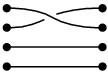
\includegraphics{pasted1} & ~~~~~~~ & 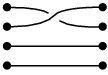
\includegraphics{pasted2}\tabularnewline
\end{tabular}\caption{Two different braids from $B_{4}.$}

\end{figure}

It is easy to see that $B_{n}$ embeds as a subgroup into $B_{n+1}$.
Additionally, if we add $\sigma_{i}^{2}=1$ for all $i=1,...,n$ in
the relations defining $B_{n}$, we obtain $\Sigma_{n}$, the permutation
group of $n$ symbols. In particular, $\Sigma_{n}$ is a finite quotient
which characterizes the infinite group $B_{n}$.

Generalizing braid groups we find Artin-Tits groups, named after Emil
Artin, due to his early work on braid groups in the 1920s to 1940s,
and Jacques Tits who developed the theory of a more general class
of groups in the 1960s. Formally speaking:
\begin{defn}
An \textbf{\index{Artin–Tits group@\textbf{Artin–Tits group}}
Artin–Tits} \textbf{group} $A$ is a finitely presented group with
presentation:
\[
A=\left\langle X\mid\left\langle x_{i},x_{j}\right\rangle ^{m_{ij}}=\left\langle x_{j},x_{i}\right\rangle ^{m_{ji}}\text{for all }x_{i}\neq x_{j}\text{ in }X\right\rangle ,
\]
where $m_{ij}\geq2$ are positive integers such that $m_{ij}=m_{ji}$
and $\left\langle s,t\right\rangle ^{k}=ststst...$ with $k$ terms
in total.

In particular, one says that an Artin–Tits group is of spherical type
when the associated \textbf{\index{Coxeter group@\textbf{Coxeter group}}Coxeter
group} (obtained by adding the relation $x_{i}^{2}$ for all $x_{i}\in X$,
to the presentation) is finite. This particular case, represents a
generalization of Braid groups, and a particular family of Garside
groups.
\end{defn}

\begin{rem}
As the reader may notice, if $X=\left\{ \variables[x]\right\} $ ,
$m_{i,j}=3$ for $\left|i-j\right|=1$ and $m_{ij}=2$ otherwise,
then presentation above $A$ is the classical presentation of the
braid group on $n+1$ strings.
\end{rem}

Within the study of Artin-Tits groups, the notions of reducible and
irreducible, soon appeared in literature. Without going into the details,
every reducible Artin-Tits groups decomposes in terms of irreducible
ones. Consequently, to describe the irreducible Artin-Tits groups
was one of the main goals of research. This task, for the special
case of Artin-Tits groups of spherical type, was finally achieved
by H.S.M. Coxeter in \cite{coxeter1935complete}. More precisely,
every irreducible Artin-Tits groups of spherical type belongs to one
of the infinite families $A_{n},B_{n},D_{n},I_{2}\left(n\right)$
or is one of the six exceptional groups $E_{6},E_{7},E_{8},F_{4},H_{3}$
and $H_{4}$.

The classification of indecomposable Artin-Tits groups of spherical
type, as implied by the existence of the 6 sporadic groups, presents
a challenging endeavor. Similarly, extending this classification to
Garside groups, which can be viewed as a broader category, also presents
a formidable open problem in the current research landscape.

\section{Garside monoids and groups}

Various equivalent representations of Garside groups exist, and numerous
generalizations have been developed since their inception. However,
in this text, we will focus solely on one particular presentation.
To understand this, we'll first need to cover some basic definitions.

\begin{defn}
A monoid $M$ is said to be \textbf{\index{right cancellative@\textbf{right cancellative}}right
cancellative} if for every $a,b,c\in M$ $a\cdot c=b\cdot c$ implies
$a=b$. Similarly, it is said to be \textbf{\index{left cancellative@\textbf{left cancellative}}left
cancellative} if for every $a,b,c\in M$ $c\cdot a=c\cdot b$ implies
$a=b$. A monoid $M$ is said to be \textbf{\index{cancellative@\textbf{cancellative}}cancellative}
if it is both left and right cancellative.
\end{defn}

\begin{rem}
We will denote by $1$ to the identity element of a monoid $M$, which
always exists.
\end{rem}

\begin{defn}
An element $a\neq 1$ in a monoid $M$ is an \textbf{\index{atom@\textbf{atom}}atom}
if for all $b,c$ in $M$ so that $a=b\cdot c$ then either $b=1$
or $c=1$.
\end{defn}


\begin{defn}
A monoid $M$ is said \textbf{\index{conical@\textbf{conical}}conical} if given $a,b\in M$ so that $a\cdot b=1$ then, $a=b=1$, i.e., no non-trivial element in $M$ has an inverse.
\end{defn}


For any element $x$ in the monoid $M$, $\parallel x\parallel$ denotes
the \textbf{norm of the element\index{norm of an element@\textbf{norm of an element}}}
$x$, supremum of the lengths of all expressions of $x$ in terms
of atoms of $M$.\nomenclature{$\parallel x\parallel$}{Norm of an element}
\begin{defn}
A monoid $M$ is said an \textbf{\index{atomic monoid@\textbf{atomic monoid}}atomic
monoid} if $M$ is generated by its atoms and $\parallel x\parallel$
is finite for all $x\in M$.
\end{defn}

\begin{defn}
If $M$ is a monoid, and the equality $a\cdot c=b$ holds for some
$a,b,c\in M$, then we say that: $a$ is a \textbf{\index{left divisor@\textbf{left divisor}}left
divisor }of $b$; $b$ is a \textbf{\index{right multiple@\textbf{right multiple}}right
multiple} of $a$; $c$ is a \textbf{\index{right divisor@\textbf{right divisor}}right
divisor} of $b$; and $b$ is a \textbf{\index{left multiple@\textbf{left multiple}}left
multiple} of $c$.
\end{defn}

Given a monoid $M$ we may consider two associated partial orders:
\[
a\leq_{L}b\text{ if }a\text{ left divides }b,
\]
\[
a\leq_{R}b\text{ if }a\text{ right divides }b.
\]

for $a,b\in M$. When every pair of elements have a supremum and a
infimum, then the partial order is said to be a lattice. For the above
partial orders, being a lattice implies that for each pair of elements
$a,b\in M$, there exist a unique \textbf{\index{least common multiple@\textbf{least common multiple}}least
common multiple}, to the left and to the right, denoted by $a\vee_{L}b$
and $a\vee_{R}b$, and also a unique \textbf{\index{greatest common divisor@\textbf{greatest common divisor}}greatest
common divisor}, to the left and to the right, denoted by $a\wedge_{L}b$
and $a\wedge_{R}b$. If $a\vee_{R}b$ is the right least common multiple
of $a,b$ then $a\vee_{R}b=ac=bd$ for some elements $c,d\in M$;
we will denote this ``right complements'' $c$ and $d$ by $a\backslash b$
and $b\backslash a$ respectively, so that $a\vee_{R}b=a(a\backslash b)=b(b\backslash a)$.\nomenclature{$\wedge_{L},\wedge_{R}$}{Greatest common divisor on the left and on the right}\nomenclature{$\vee_{L},\vee_{R}$}{Least common multiple on the left and on the right}

\begin{defn}
An element $\Delta$ \nomenclature{$\Delta$}{Garside element} in
$M$ is said \textbf{\index{balanced@\textbf{balanced}}balanced}
if the sets of left divisors and right divisors coincide, and the
\textbf{\index{set of divisors@\textbf{set of divisors}}set of divisors}
is denoted by \nomenclature{$\text{Div}\left(\Delta\right)$}{Set of divisors of $\Delta$}$\text{Div}\left(\Delta\right)$. 
\end{defn}

\begin{defn}
\cite[0.5.1]{bessis_dual_2003} A monoid $M$ is a \textbf{\index{Garside monoid@\textbf{Garside monoid}}Garside
monoid} when:
\begin{enumerate}
\item $M$ is cancellative.
\item $M$ is atomic. 
\item $\leq_{R}$ and $\leq_{L}$ are both lattices in $M$.
\item There exists an element $\Delta\in M$, called \textbf{\textit{\index{Garside element@\textbf{Garside element}}}}\textbf{Garside
element} of $M$, such that:
\begin{enumerate}
\item It is balanced.
\item The set of divisors of $\Delta$ is finite and generates $M$.
\end{enumerate}
\end{enumerate}
\end{defn}

\begin{rem}
Conditions 1,2 and 3 define the so called \textbf{\index{Gaussian monoids@\textbf{Gaussian monoids}}Gaussian
monoids}, thus a Garside monoid is a Gaussian monoid with a Garside
element.  
\end{rem}

 Because Garside groups satisfy Ore's condition, every Garside monoid
$M$ satisfies embeds in its group of fractions, see \cite{dehornoy99gaussian_and_garside}
or alternatively \cite[1.23]{clifford1961algebraic}.
\begin{defn}
A \textbf{\index{Garside group@\textbf{Garside group}}Garside group}
is the group of fractions of a Garside monoid.
\end{defn}

When there is no ambiguity,\nomenclature{$G^{+}$}{Underlying Garside monoid}
$G^{+}$ will represent the underlying Garside monoid of a given Garside
group $G$, and in some occasions, the elements of $G^{+}$ are referred
to as positive elements. An immediate consequence of the definition is that Garside monoids are conical, that is, no element different from the identity has inverse, otherwise $\parallel 1\parallel$, the norm of the identity, would not be bounded, in contradiction with  $G^+$ being an atomic monoid. However, this turns out to be a good property and Garside groups work as expected
with respect its underlying Garside monoid.

\begin{comment}
	When there is no ambiguity,\nomenclature{$G^{+}$}{Underlying Garside monoid}
	$G^{+}$ will represent the underlying Garside monoid of a given Garside
	group $G$, and in some occasions, the elements of $G^{+}$ are referred
	to as positive elements. It is a simple fact that $G^{+}$ is a \textbf{\index{conical@\textbf{conical}}conical}
	monoid, that is, if $a,b\in G^{+}$ are so that $a\cdot b=1$ then
	$a=b=1$, i.e., no non-trivial element in $G^{+}$ has an inverse.
	This turns out to be a good property and Garside groups work as expected
	with respect its underlying Garside monoid.
\end{comment}


\begin{lem}
\cite[1.11]{godelle07parabolic} Let $G$ be a Garside group. For
every element $g$ in the group $G$ there exists a unique pair $(a,b)$
of elements in the monoid $G^{+}$ such that $g=a^{-1}b$ and the
elements $a$ and $b$ are coprime for left divisibility. Furthermore
if $cg$ lies in $G^{+}$for some $c$ in $G^{+}$then $a$ right
divides $c$.
\end{lem}

\begin{lem}
\cite[3.1]{doi:10.1081/AGB-100001665} Let $G$ be a Garside group.
Let $a,b$ be conjugate elements in $G$, then $a,b$ are also conjugated
by an element in $G^{+}$.
\end{lem}

Before we conclude this section, it's worth noting that alternative
definitions of Garside groups can be found in the literature (see
\cite{dehornoy99gaussian_and_garside,Dehornoy2002,godelle07parabolic,PICANTIN200192}),
however we followed the lines of \cite{chouraqui_garside_2010} instead.
Additionally, other definitions regarding other structures can also be
found in literature, see for instance \cite{picantin2005garside}, where alternative definitions using divisibility monoids are made.  

A simple fact about Garside elements is that if $\Delta_{1},\Delta_{2}$
are Garside elements so is its greater common divisor, and so, every
Garside monoid has a minimal Garside element with respect to divisibility.
Another result, first proven by P. Dehornoy in \cite{Dehornoy2002}
is if $\Delta$ is a Garside element, then so is $\Delta^{n}$ for
every natural number $n\geq1$, although it can be seen as a direct
consequence of some results from \cite{PICANTIN200192}. 

It is known that the Garside element of a Garside monoid $M$, induces
a permutation on the set of atoms of $M$, that is, given an atom
$a$ we have $a\Delta=\Delta b$ for some atom $b$ (see \cite[2.6]{dehornoy99gaussian_and_garside}).
Hence, since the set of atoms is finite, there exists a positive integer
$e$ so that $\Delta^{e}$ in a central element. This power $e$ is
usually referred to as the \textbf{\index{exponent of the monoid@\textbf{exponent} \textbf{of the monoid}}exponent}
\textbf{of the monoid}.
\begin{thm}
\cite[3.17]{lee11periodic} Let $G$ be a Garside group with Garside
element $\Delta$ and let $e$ be the exponent of the monoid $G^+$. Then every finite subgroup of
$G/\left\langle \Delta^{e}\right\rangle $ is cyclic.
\end{thm}

Next result shows that Garside groups have finite abelian subgroup
rank.
\begin{prop}
\cite[3.5]{lee06abelian} If $H$ is an abelian subgroup of a Garside
group $G$, then $$\left|N_{G}\left(H\right):C_{G}\left(H\right)\right|<\infty.$$
\end{prop}



\begin{prop}\label{abelian_subgroups_are_fg}
\cite{Charney2004} Every abelian subgroup of a Garside group is finitely
generated.
\end{prop}

\begin{comment}
\begin{prop}
	\cite{Charney2004} Every Garside group has finite virtual cohomological dimension, hence every abelian subgroup of a Garside group is finitely
	generated.
\end{prop}
\end{comment}

The above result is generalized by  \myref[Corollary]{cor:solvable Lee then virtually abelian},
which states that every solvable subgroup of a Garside group is finitely
generated and virtually abelian.

\begin{defn}
Two elements $x,y$ in a monoid are said \textbf{\index{commensurable@\textbf{commensurable}}commensurable}
if there exist positive integers $k,r$ so that $x^{k}$ and $y^{r}$
are conjugated.
\end{defn}

\begin{thm}
\label{thm:commensurable}\cite[3.1]{lee11periodic} Let $G$ be a
Garside group. Then $Z\left(G\right)$ is cyclic if and only if for
every pair of Garside elements $\Delta_{1},\Delta_{2}$ of $G$ are
commensurable.
\end{thm}

Garside groups with cyclic center play a central role in Garside group
theory, as we shall see later on.

\section{Some examples of Garside groups}

Two classical examples of Garside Groups are: Braid groups and Artin-Tits
groups of spherical type. 
\begin{example}
\cite[Example \#4]{dehornoy99gaussian_and_garside} Given $n$ positive
integers $p_{1},...,p_{n}$, the group defined by 
\[
\left\langle \variables[x][n]|x_{1}^{p_{1}}=x_{2}^{p_{2}}=...=x_{n}^{p_{n}}\right\rangle ,
\]
is a Garside group with Garside element $\Delta=x_{1}^{p_{1}}$. In
particular, $pq$-Torus knot groups presented by $\left\langle x,y|x^{p}=y^{q}\right\rangle $
is a family of Garside groups. 
\end{example}

\begin{example}
The group $G=\left\langle a,b|aba=b^{2}\right\rangle $ is a Garside
group with minimal Garside element $\Delta=abab=b^{3}$. Notice that
$aba$ is the least common multiple to the left and to the right for
the atoms $a,b$, but is not a Garside element since $ab$ is a left
divisor but not a right divisor.

In example above, if $x=ab$ and $y=b$, then $x,y$ generate the
group and satisfy the relation $x^{2}y^{-1}=y^{2}$, that is $x^{2}=y^{3},$
and so it is a $2,3$-Torus knot group. Thus, one Garside group can
have different presentations. 
\end{example}

\begin{example}
Another simple example is the Garside group (see \cite[p 228]{birman2007conjugacy}
or \cite[4.2]{PicantinThesis})
\[
G=\left\langle a,b\mid ababa=b{{}^2}\right\rangle ,
\]
its minimal Garside element is $\Delta=b^{3}$. In this case, we see
that relations defining the group are not length preserving. However,
if we take $x=ab$ and $y=b$, then $x^{3}y^{-1}=ababa=b^{2}=y^{2}$
and $x^{3}=y^{3}$. Thus we can provide, in this case, a different
presentation that is length preserving.
\end{example}

\begin{rem}
In the present text we won't deal with problems regarding different
presentations and shall always consider a fixed presentation for a
Garside group.
\end{rem}

\begin{example}
The Artin-Tits Group $G=\left\langle a,b\mid aba=bab\right\rangle $
has $\Delta=aba$ as non central Garside element and $Z\left(G\right)=\left\langle \Delta^{2}\right\rangle $.
That is, it has exponent $2$.
\end{example}


\section{Garside subgroups and parabolic subgroups}

The notions of parabolic and Garside subgroups was introduced by E.
Godelle in \cite{godelle07parabolic}. In that article the notion
of quasi-Garside is used, which allows to the set of divisors of the
Garside element, $\text{Div\ensuremath{\left(\Delta\right)}}$, to
be infinite. However, since we only deal with the finite case, we
have omitted the term quasi-Garside in the statement of the results.
\begin{defn}
Given a Garside group $G$ and a balanced element $\delta$ of $G^{+}$,
the \textbf{support\index{support@\textbf{support}}} of $\delta$
is the set $\text{Supp}_{G^{+}}\left(\delta\right)$ of atoms of $G^{+}$
that are in $\text{Div}\left(\delta\right)$. \nomenclature{$\text{Supp}_{G^{+}}\left(\delta\right)$}{Set of atoms of $G^{+}$ dividing $\delta$}
\end{defn}

\begin{defn}
\cite[1.6]{godelle07parabolic} Let $G$ be a Garside group with Garside
element $\Delta$, and $H$ be a subgroup of $G$. Set $H^{+}=H\cap G^{+}$.
We say that the subgroup $H$ is a \textbf{\index{Garside subgroup@\textbf{Garside subgroup}}Garside
subgroup} of the group $G$ if:
\begin{enumerate}
\item the submonoid $H^{+}$ is a closed sublattice of the monoid $G^{+}$;
\item for every $x\in H^{+},$ the elements of $G^{+}$ $x\wedge_{L}\Delta$,$x\wedge_{R}\Delta$
are also in $H^{+}$;
\item the subgroup $H$ is generated by the submonoid $H^{+}$.
\end{enumerate}
\end{defn}

\begin{rem}
Definition above implies that the Garside subgroup structure is related
with the structure within it exits. Additionally, notation above for
$H^{+}$ is coherent with the fact that $H$ is the group generated
by $H^{+}$. 
\end{rem}

\begin{prop}
\cite[1.15]{godelle07parabolic} Let $G$ be a Garside group with
Garside element $\Delta$. Let $H$ be a Garside subgroup of $G$.
Then, we have
\[
\mathrm{N}_{G}(H)=H^{+}\cdot\mathrm{N}_{G}\left(H^{+}\right).
\]
\end{prop}

\begin{prop}
\cite[1.14]{godelle07parabolic} Let $G$ be a Garside group and let
$H$ and $K$ be two Garside subgroups of $G$. Then, the subgroup
$H\cap K$ is a Garside subgroup of the group $G$ and the submonoid
$(H\cap K)\cap G^{+}$is equal to the submonoid $H^{+}\cap K^{+}$.
\end{prop}

\begin{thm}
\cite[1.10]{godelle07parabolic} Let $G$ be a Garside group with
Garside element $\Delta$, and let $H$ be a Garside subgroup of $G$.
Set $H^{+}=H\cap G^{+}$.
\begin{enumerate}
\item The subset $H^{+}\cap\text{Div}(\Delta)$ is a closed sublattice of
$G^{+}$. In particular, there exists an element $\delta$ in $H^{+}$that
is balanced in $H^{+}$and such that $H^{+}\cap\text{Div}(\Delta)=\text{Div}_{H^{+}}(\delta)$.
\item $H$ is a Garside group with Garside element $\delta$ and $H^{+}$
as underlying Garside monoid.
\end{enumerate}
\end{thm}

\begin{defn}
\cite[2.2]{godelle07parabolic} Let $G$ be a Garside group with Garside
element $\Delta$. 
\begin{enumerate}
\item Let $\delta$ be a balanced element of $\text{Div}(\Delta)$. Denote
by \nomenclature{$G_{\delta}$}{Subgroup generated by $\text{Supp}_{G^{+}}(\delta)$}
$G_{\delta}$ the subgroup of $G$ generated by $\text{Supp}_{G^{+}}(\delta)$.
We say that $G_{\delta}$ is a \textbf{\index{standard parabolic subgroup@\textbf{standard parabolic subgroup}}standard
parabolic subgroup} of the group $G$ if $\text{Div}(\delta)=$ $\text{Div}(\Delta)\cap G_{\delta}^{+}$.
In that case, the monoid $G_{\delta}^{+}$ is called a \textbf{\index{parabolic submonoid@\textbf{parabolic submonoid}}parabolic
submonoid} of the monoid $G^{+}$.
\item Let $H$ be a subgroup of $G$. We say that $H$ is a \textbf{parabolic
subgroup\index{parabolic subgroup@\textbf{parabolic subgroup}}} of
$G$ if it is conjugated to a standard parabolic subgroup of $G$.
\end{enumerate}
\end{defn}

\begin{rem}
Notice that in theorem above, unlike in the previous definition, the
element $\delta$ is balanced in the Garside submonoid, but not necessarily
balanced in $G^{+}$. The significance of this will be highlighted
in subsequent discussions.
\end{rem}

\begin{lem}
\cite[2.1]{godelle07parabolic} Let $G$ be a Garside group with Garside
element $\Delta$. Let $\delta$ be a balanced element of $\text{Div}(\Delta)$;
we denote by $H$ the subgroup of $G$ generated by $\text{Supp}{}_{G^{+}}(\delta)$,
and we set $H^{+}=H\cap G^{+}$. Then $H$ is a Garside group with
Garside element $\delta$ and $\text{Supp}_{G^{+}}(\delta)$ as set
of atoms. Furthermore, the subgroup $H$ is a Garside subgroup with
$\delta$ as Garside element if and only if the equality $\text{Div}(\delta)=\text{Div}(\Delta)\cap H^{+}$holds
in $G^{+}$.
\end{lem}

We can derive two consequences of theorem above:
\begin{enumerate}
\item Standard parabolic subgroups are indeed Garside subgroups.
\item Garside groups within a Garside group may not necessarily be related
with the group's overall structure. Therefore, a subgroup being Garside
is not the same as being a Garside subgroup.
\end{enumerate}
In the same article, \cite[3.4,3.5.3.5,3.8]{godelle07parabolic},
many questions are asked and answered, in all cases with a negative
answer. The following is a compilation of them:

\textcompwordmark{}

Let $G$ be a Garside group with Garside element $\Delta$. Let $X$
denote the set of atoms of $G^{+}$ and for $Y\subseteq X$ a set
of atoms of the monoid $G^{+}$, denote by $G_{Y}^{+}$\nomenclature{$G_{Y}^{+}$}{Submonoid generated by Y}
the submonoid generated by $Y$. Additionally, let $\delta$ be a
balanced element of $\text{Div}(\Delta)$.
\begin{enumerate}
\item Is the subgroup $G_{Y}^{+}$ necessarily a Garside subgroup? 
\begin{enumerate}
\item If the subgroup $G_{Y}^{+}$ is a Garside group, is it necessarily
a Garside subgroup?
\item If the subgroup $G_{Y}^{+}$ is a Garside subgroup, is it necessarily
a (standard) parabolic subgroup?
\item Are $\text{Div}(\Delta)\cap G_{\delta}^{+}$ and $\text{Div}(\delta)$
necessarily equal?
\item Do we have necessarily a one-to-one correspondence between the balanced
elements in $\text{Div}(\Delta)$ and the standard parabolic subgroups?
\item Is the intersection of two Garside subgroups generated by sets of
atoms necessarily (a Garside subgroup) generated by a set of atoms?
\end{enumerate}
\end{enumerate}
%
In so far, we have seen that the class of Garside groups strictly
contains the class of Garside subgroups, which also strictly contains
the class of (standard) parabolic subgroups. Therefore, since these
notions differ, one should inquire about the special properties associated
with each of them. The following can be taken as an approximation
to the this problem.
\begin{lem}
\cite[1.9]{godelle07parabolic} Let $G$ be a Garside group with Garside
element $\Delta,$ and $H$ be a Garside subgroup of $G$. Set $H^{+}=H\cap G^{+}$.
Let $h_{1},h_{2}$ belong to $H^{+}$. Then the element $h_{1}$ is
a left (right) divisor of $h_{2}$ in $H^{+}$ if and only if $h_{1}$
is a left (right) divisor of $h_{2}$ in $G^{+}$.
\end{lem}

While one implication is trivial, the non-trivial part is far from
trivial since, in Garside monoids, one element can have many possible
words in terms of atoms, even of different lengths. One intuitive
way, and likely easy, to approach this property relates with its Garside
element: since the Garside subgroup $H$ satisfies, by definition,
that every common divisor of an arbitrary element of $H^{+}$and the
Garside element $\Delta\in G^{+}$ belongs to $H^{+}$, this properties
extends from the Garside element $\Delta$ to the whole Garside monoid
$G^{+}$. One way to rephrase the previous is: ``from the Garside
element to the Garside monoid''. Although this is not a rigorous
mathematical claim, it feels intuitive and will be repeated later
on.

Now is the turn of parabolic submonoids:
\begin{prop}
\label{prop: convex parabolic}\cite[2.5]{godelle07parabolic} Let
$G_{\delta}^{+}$ be a parabolic submonoid of a Garside monoid $G^{+}$.
Then $G_{\delta}^{+}$ is closed under left divisibility and under
right divisibility. That is, if $g\in G^{+}$ is such that $g$ left
divides, or right divides, some $x\in G_{\delta}^{+}$, then $g\in G_{\delta}^{+}$.
\end{prop}

Result above is an strong version of the previous result for Garside
subgroups. Now, for the case of parabolic subgroups, not only the
divisibility relation is inherited, but also the element dividing.
Similarly as before, we see from its definition, if $G_{\delta}^{+}$
is a  parabolic submonoid, the relation $\text{Div}(\delta)=$ $\text{Div}(\Delta)\cap G_{\delta}^{+}$
is satisfied, and thus, the divisors of $\delta$ and $\Delta$ are
shared in $G_{\delta}^{+}$. In some sense, the sentence ``from the
Garside element to the whole monoid'', applies again for the previous
proposition.

\begin{prop}
\label{prop:standar parabolic intersectio} \cite[2.7]{godelle07parabolic}
Let $G$ be a Garside group, and $G_{\delta}$, $G_{\tau}$ be two
standard parabolic subgroups of $G$. Then $G_{\delta\wedge\tau}$
is a standard parabolic subgroup of $G$, which is equal to the subgroup
$G_{\delta}\cap G_{\tau}$.
\end{prop}

Unfortunately, for the join of two standard parabolic subgroups no
similar result is known. In the next sections we shall see a way to
create bigger Garside groups starting with two Garside, so that they
become standard parabolic subgroups of the new structure. 

In \cite{CUMPLIDO2019572} the following is said: ``We show that,
in an Artin–Tits group of spherical type, the intersection of two
parabolic subgroups is a parabolic subgroup. Moreover, we show that
the set of parabolic subgroups forms a lattice with respect to inclusion.
This extends to all Artin–Tits groups of spherical type a result that
was previously known for braid groups''.

\textcompwordmark{}

\textbf{Question}. Can the previous mentioned be generalized to the
context of Garside groups?

\section{Irreducible Garside monoids}

Concerning parabolic subgroups and Artin-Tits groups, there exists
the concept of irreducible Garside monoids, which serve as a natural
extension of irreducibility in Artin-Tits monoids to the realm of
Garside groups. This accomplishment was made by Matthieu Picantin
in \cite[Theorem B]{PICANTIN200192}, where he successfully described
all Garside monoids as a sequence of \textquotedbl crossed products\textquotedbl{}
of Garside parabolic submonoids. However, we will forgo detailing
the crossed product concept due to its high level of complexity and
technicality. It was later shown to be equivalent to the Zappa-Szép
product, which we will introduce later in the text.\\

Based on the fact the every Garside element $\Delta$ acts on the
monoid, that is, given $a\in G^{+}$ there exists $b\in G^{+}$ so
that $a\Delta=\Delta b$, M. Picantin introduced the quasi-center
of a Garside monoid, which comprises the set elements behaving like
$\Delta$. Formally:
\begin{defn}
\cite[B]{PICANTIN200192} Assume that $M$ is a Garside monoid, $X$
is its set of atoms, and $G$ is its group of fractions. Then the
\textbf{\index{quasi-center@\textbf{quasi-center}}quasi-center} of
$M$ (resp. the \textbf{\index{quasi-centralizer@\textbf{quasi-centralizer}}quasi-centralizer}
of $X$ in $G$) is the submonoid \nomenclature{$QZ\left(M\right)$}{Quasi-center of the Garside monoid $M$}$QZ\left(M\right)=\left\{ x\in M|\text{given }a\in X,\text{exists }b\in X\text{ so that }xa=bx\right\} $
(resp. the subgroup \nomenclature{$QZ\left(G\right)$}{Quasi-centralizer of $X $ in the Garside group $G$}$QZ\left(G\right)=\left\{ x\in G|\text{given }a\in X,\text{exists }b\in X\text{ so that }xa=bx\right\} $).
\end{defn}

\begin{lem}
\cite[1.8]{PICANTIN200192} Assume that $M$ is a Garside monoid,
$X$ is the set of its atoms, and $G$ is its group of fractions.
Then:
\begin{enumerate}
\item the quasi-centralizer of $X$ in $G$ is the group of fractions of
the quasi-center of $M$;
\item the center of $G$ is the group of fractions of the center of $M$.
\end{enumerate}
\end{lem}

\begin{defn}
\label{def:definitiongeneratorquasicenter}Assume that $M$ is a Garside
monoid. For every $a$ in $M$, we define \nomenclature{$\Delta_{a}$}{Generator of the quasi-center}
\[
\Delta_{a}=\vee_{R}\left\{ b\backslash a;b\in M\right\} .
\]
\end{defn}

Notice that a similar definition can be made by means of the left
least common multiple $\vee_{L}$, however, they turn out to be equivalent
by \cite[2.13]{PICANTIN200192}.

Moving forward, we will explore a number of key findings and definitions
from the same article, which will prove to be significant later on.
\begin{prop}
\label{prop: Picantin Popurri}\cite[2.2,2.6,2.7,2.8,2.9,1.7]{PICANTIN200192}
Let $M$ be a Garside monoid and $a$ an element of $M$. Then:
%\begin{enumerate}
\item The element $\Delta_{a}$ is quasi-central. More precisely, the application
$a\mapsto\Delta_{a}$ is a surjection from $M$ onto the quasi-center
of $M$.
\item If $\Delta_{a}=a$ then $a$ is quasi-central.
\item If $a$ divides a quasi-central element $b$ in $M$, then $\Delta_{a}$
and divides $b$. 
\item The set $\left\{ \Delta_{x}\mid x\text{ atom of }M\right\} $ is basis
for the quasi-center of $M$.
\item Either $\Delta_{a}=\Delta_{b}$ or $\Delta_{a}\wedge\Delta_{b}=1$
for $b$ in $M$. 
\item The quasi-center is closed under $\vee$ and $\wedge$.
\item $\Delta_{a}\vee\Delta_{b}=\Delta_{a\vee b}$.
\item Every element of the quasi-center is a balanced element.
\end{enumerate}
\end{prop}

\begin{rem}
Although $\vee$ and $\wedge$ should have been considered also to
the left and to the right, for elements in the quasi-center these
notions turn out tho be equivalent by definition.
\end{rem}

Different characterizations of irreducible Garside monoids exists,
but from a chronological point of view, the first definition of irreducible
Garside monoid is the following one: a Garside monoid is \textbf{irreducible\index{irreducible Garside monoid@\textbf{irreducible Garside monoid}}}
if $\Delta_{a}=\Delta_{b}$ for every atom $a,b$ of $G^{+}$. 
\begin{prop}
\cite[4.1]{PICANTIN200192} Let $G^{+}$ be an irreducible Garside
monoid with minimal Garside element $\Delta$. Denote by $e$ is its
exponent, and $G$ is its group of fractions. Then:
\begin{enumerate}
\item The quasi-center of $G^{+}$ is the infinite cyclic submonoid generated
$\Delta$.
\item The center of $G^{+}$ (resp. of $G$) is the infinite cyclic submonoid
(resp. subgroup) generated by $\Delta^{e}$. 
\end{enumerate}
\end{prop}


\section{Zappa-Szép decompositions}

In order to solve some problems regarding Picantin's crossed-product,
in \cite{Gebhardt2016} the authors study the Zappa-Szép product of
monoids for the case of Garside monoids, showing that in this case
they are equivalent.
\begin{defn}
A monoid $M$ is the (internal) \textbf{Zappa-Szép product\index{Zappa-Szép product@\textbf{Zappa-Szép product}}\nomenclature{$\bowtie$}{Zappa-Szép product}}
of two submonoids $A$ and $B$, $M=A\bowtie B$, if every element
$x\in M$ can be uniquely written as $x=a\cdot b=b'\cdot a'$, with
$a,a'\in A$, $b,b'\in B$.
\end{defn}

It is easy to see that Zappa-Szép product generalized direct and semidirect
product for monoids. If $G^{+}=H^{+}\bowtie K^{+}$ is a Garside monoid,
then the Garside group $G$ can be presented as
\[
G=\left\{ h_{1}k_{1}k_{2}^{-1}h_{2}^{-1}\mid h_{i}\in H^{+},k_{i}\in K^{+},\,\,i=1,2\right\} .
\]

\begin{defn}
A Garside monoid is an\textbf{ \index{indecomposable Garside monoid@\textbf{indecomposable} \textbf{Garside} \textbf{monoid}}indecomposable}
\textbf{Garside} \textbf{monoid}, if it cannot be written as a Zappa-Szép
product of two non-trivial submonoids.
\end{defn}

Next results allow us to avoid Picantin's crossed product.
\begin{thm}
\cite[39]{Gebhardt2016} A Garside monoid $M$ is irreducible if and
only if it is (Zappa-Szép) indecomposable.
\end{thm}

Actually, the notion of crossed product introduced by Picantin, is
equivalent, for Garside monoids, to the notion of Zappa-Szép product
as the following result shows.
\begin{thm}
\cite[33]{Gebhardt2016} If $G^{+}$ is a Garside monoid with submonoids
$H^{+}$ and $K^{+}$, one has $G^{+}=H^{+}\bowtie K^{+}$ if and
only if $G^{+}$ can be written as a crossed product of the monoids
$H^{+}$ and $K^{+}$.
\end{thm}

\begin{rem}
It is a easy fact that the set of atoms of $G^{+}$ is the disjoint
union of the sets of atoms of $H^{+}$ and $K^{+}$. For that, take
$a$ an atom of $G^{+}$ and write $a=hk$ for some $h\in H^{+}$,
$k\in K^{+}$, then being an atom implies either $h=1$ or $k=1$,
and so $a$ is a atom of $H^{+}$ or $K^{+}$. So far we know that
if $G^{+}$ is not an indecomposable monoid, it can be written as
the product of two Garside submonoids $H^{+}$ and $K^{+}$. Now we
can repeat the same argument for $H^{+}$,$K^{+}$ if they are not
indecomposable and continue applying this argument recursively. Because
the set of atoms of $G^{+}$ is finite, we are ensured that this process
terminates, and we obtain a decomposition in terms of finitely many
indecomposable Garside submonoids. Unfortunately, this Zappa-Szép
decomposition is not associative, and so, not necessarily unique. 

Usually, we will denote this indecomposable Garside submonoids by
$H_{1},...,H_{n}$, and will consider them in order from left to right
on the (recursive) decomposition of $G^{+}$, which we shall not specify.
\end{rem}

\begin{rem}
We know that a Garside monoid is by definition generated by the set
of divisors of the Garside element $\Delta$. Thus, $\Delta$ can
be written as the product of atoms (irreducible elements). Similarly,
by results above we have that the whole Garside monoid can be written
as the product of some irreducible Garside submonoids generated by
some disjoint subsets of atoms of $G$. Thus, the analogy: ``from
the Garside element to the Garside monoid'' is again satisfied.
\end{rem}

\begin{lem}
\cite[4.5]{lee11translation} If $\delta_{H}$ and $\delta_{K}$ are
the minimal Garside elements of $H^{+}$ and $K^{+}$, respectively,
then $\delta_{H}\cdot\delta_{K}$ is the minimal Garside element of
$H^{+}\bowtie K^{+}$.
\end{lem}

\begin{thm}
\label{thm:gebhradt tawn parabolic}\cite[34]{Gebhardt2016} If $G^{+}=H^{+}\bowtie K^{+}$
is a Garside monoid, then $H^{+}$ and $K^{+}$ are parabolic submonoids
of $G^{+}$. In particular, $H^{+}$ and $K^{+}$ are Garside monoids.
Additionally, factorization of a Garside element $\Delta$ of $G^{+}$,
$\Delta=\Delta_{H}\Delta_{K}$, produces Garside elements of $\Delta_{H}$
of $H^{+}$ and $\Delta_{K}$ of $K^{+}$.
\end{thm}

It is not always true that the product of Garside elements of the
monoids $H^{+}$ and $K^{+}$ produces a Garside element of $G^{+}$
(see \cite[36]{Gebhardt2016}).
\begin{lem}
\cite[17]{Gebhardt2016} \label{lem:divisor_belongs_to_H} Suppose
that $G^{+}=H^{+}\bowtie K^{+}$ and that $H^{+}$ is conical. Then,
for all $x,y\in G^{+}$, $xy\in K^{+}$ implies that $x\in K^{+}$
and $y\in K^{+}$. Consequently, if $h\in H^{+}$, every divisor of
$h$ belongs to $H^{+}$.
\end{lem}

\begin{lem}
\cite[18]{Gebhardt2016} \label{lem:swapping_atoms_gives_atoms} Suppose
that $G^{+}=H^{+}\bowtie K^{+}$ and that $H^{+}$ is conical. Let
$g\in G^{+}$ and write its factorization as $g=ha=bh'$ with $h,h'\in H^{+}$
and $a,b\in K^{+}$. If $a$ is an atom of $K^{+},$then so is $b$.
\end{lem}

\begin{rem}
By definition, every Garside monoid $G^{+}$ is conical, thus so are
$H^{+}$ and $K^{+}$. Thus, there is not additional hypothesis when
$G^{+}$ is a Garside monoid.
\end{rem}

\begin{prop}
\cite[35]{Gebhardt2016} Let $G^{+}=H^{+}\bowtie K^{+}$ be a Garside
monoid and let $k\in K^{+}$. Then $\Delta_{k}^{G^{+}}=\bigvee\{x\backslash k$
: $x\in G^{+}\}\in K^{+}$.\label{prop:lcm in G and K coincide}
\end{prop}

\begin{thm}
\cite[37]{Gebhardt2016} Suppose that $G^{+}=H^{+}\bowtie K^{+}$
and that $H^{+}$ and $K^{+}$ are Garside monoids. Then $G^{+}$
is a Garside monoid.
\end{thm}

Before to proceed, we shall recall some results from the previous
chapter in order to facilitate the reader the understanding of some
proofs.
\begin{prop}
\cite{PICANTIN200192}\label{prop:Picantin} Let $G$ be a monoid,
then:
\begin{enumerate}
\item If $ab=ba$ and $a\wedge_{R}b=1$, then $ab=a\vee b$.
\item If $b\in QZ\left(G\right)$ and $a\in G$ divides $b$, then $\Delta_{a}$
divides $b$.
\item $QZ\left(G\right)$ is closed under $\vee$ and $\wedge$.
\item Every element of $QZ\left(G\right)$ is a balanced element.
\end{enumerate}
\end{prop}


\section{Free groups and HNN extensions}

In this section we shall see a different kind of product of Garside
monoids. They were introduce by Matthieu Picantin in \cite{picantin2013tree}
and remarkably, the class of Garside groups is closed under this product
(alternatively, extensions).
\begin{defn}
Let $M_{1},M_{2},H$ be monoids with morphisms $\phi_{1}:H\hookrightarrow M_{1}$
and $\phi_{2}:H\hookrightarrow M_{2}$. The \textbf{\index{amalgamated free product@\textbf{amalgamated free product}}amalgamated
free product} of $M_{1}$ and $M_{2}$ with respect to $H,\phi_{1}$,
and $\phi_{2}$ is the monoid 
\[
\left\langle M_{1}\star M_{2}:\phi_{1}(h)=\phi_{2}(h),h\in H\right\rangle ^{+},
\]
where $M_{1}\star M_{2}$ stands for the free product of $M_{1}$
and $M_{2}$. When $H=\langle h\rangle^{+}$is cyclic, we denote $\phi_{1}(h)=h_{1},\phi_{2}(h)=h_{2}$,
and the \textbf{\index{cyclic amalgamated free product@\textbf{cyclic amalgamated free product}}cyclic
amalgamated free product} $M_{1}\star_{h_{1}=h_{2}}M_{2}$.
\end{defn}

For the first result regarding such product, we recall that a root
of an element $x$ is an element $h$ so that there exists a positive
integer $k$ so that $h^{k}=x$.
\begin{thm}
\cite[16]{picantin2013tree} Let $M_{1}$ and $M_{2}$ be some Garside
monoids. Then, for any root $h_{1}$ of any Garside element in $M_{1}$
and any root $h_{2}$ of any Garside element in $M_{2}$, the cyclic
amalgamated free product $M_{1}\star_{h_{1}=h_{2}}M_{2}$ is a Garside
monoid. 

Actually, a necessary assumption is that $\phi_{i}(H)$ has to contain
a Garside element of $M_{i}$ for $i\in\{1,2\}$. When restricted
to cyclic amalgamated submonoids, the latter naturally expresses in
terms of roots of Garside elements.
\end{thm}

\begin{cor}
\cite[23]{picantin2013tree} Let $M_{1}$ and $M_{2}$ be some Garside
monoids. The (enveloping group of) the cyclic amalgamated free product
$M_{1}\star_{h_{1}=h_{2}}M_{2}$ is Garside if and only if $h_{1}$
is a root of some Garside element in $M_{1}$ and $h_{2}$ is a root
of some Garside element in $M_{2}$. 
\end{cor}

\begin{defn}
Let $M$ and $H$ be two monoids with morphisms $\phi_{1}:H\hookrightarrow M$
and $\phi_{2}:H\hookrightarrow M$. The \textbf{\index{HNN extension@\textbf{HNN extension}}HNN
extension} of $M$ with respect to $H,\phi_{1}$, and $\phi_{2}$
is the monoid 
\[
\left\langle M,t:\phi_{1}(h)t=t\phi_{2}(h),h\in H\right\rangle ^{+}.
\]

For the following result, we recall that if $x$ is an element in
a Garside monoid $G^{+}$, then $\left\Vert x\right\Vert $ is the
supremum of the lengths of every possible word for $x$.
\end{defn}

\begin{thm}
\cite[26]{picantin2013tree} Let $M$ be a Garside monoid and $H$
be the infinite cyclic monoid $\langle h\rangle^{+}$with a morphism
$\phi_{i}:H\hookrightarrow M$ for $i\in\{1,2\}$ satisfying $\left\Vert \phi_{1}(h)\right\Vert =\left\Vert \phi_{2}(h)\right\Vert $.
Then the enveloping group of the HNN extension $\left\langle M,t:\phi_{1}(h)t=t\phi_{2}(h)\right\rangle ^{+}$is
a Garside group if and only if $\phi_{1}(h)$ and $\phi_{2}(h)$ are
two $n$-th roots of the same Garside element in $M$ for some $n>0$.
\end{thm}

Here again, a necessary assumption is actually that $\phi_{1}(H)$
and $\phi_{2}(H)$ have to contain the same Garside element of $M$.
When restricted to cyclic HNN extensions, the case when $H$ is cyclic,
the latter naturally expresses in terms of roots of Garside elements.

\textcompwordmark{}

Despite the great results achieved by Picantin, as the reader may
know, free products are quite difficult to deal with and few properties
can be easily derived from results above. In particular, this thesis
does not contain any new results following this line. Finally, we
end this section with two remarkable results proven by means of the
HNN extensions.

\begin{prop}
\cite[35]{picantin2013tree} A non-cyclic one-relator group is Garside
if and only if its center is non-trivial.
\end{prop}


\section{Computational properties}

This section is devoted to summarize some of the literature regarding
Garside monoids ``good monoids'', in particular, some of the common
computational problems can be achieved and besides some other properties
regarding monoids. The reader is expected to be already familiarized
with Garside monoids, and no formal definitions are included in this
section since a reference is always provided.

In \cite{dehornoy99gaussian_and_garside} is proved for Garside groups:
``the language of normal forms is regular, symmetric, and geodesic,
has the 5-fellow traveler property, and has the uniqueness property,
implying that Garside groups are geodesically fully biautomatic''. 

In \cite{Dehornoy2002} is proved that all Garside Groups are biautomatic
meaning that normal forms can be computed by means of a finite automaton.
\begin{thm}
\cite[3.4]{doi:10.1081/AGB-100001665} The conjugacy problem in Garside
groups is solvable.
\end{thm}

\begin{prop}
\cite[2.5]{sibert2004tame} If $G$ is the group of fractions of a
tame Garside monoid, then the problem of existence of $n$-th roots
in $G$ is decidable.
\end{prop}

\begin{prop}
\cite{lee06abelian} Every abelian subgroup of a Garside group is
torsion-free and finitely generated.
\end{prop}

\begin{prop}
\cite{DEHORNOY1998291} Every Garside group is torsion-free.
\end{prop}

\begin{cor}
\label{cor:solvable Lee then virtually abelian}\cite[7.3]{lee11translation}
Let $G$ be a Garside group. 
\begin{enumerate}
\item Every solvable subgroup of $G$ is finitely generated and virtually
abelian. 
\item $G$ cannot contain subgroups isomorphic to the additive group of
rational numbers or the group of $p$-adic fractions $\mathbb{Q}_{p}=\left\{ k/p^{l}\mid k\in\mathbb{Z},l\in\mathbb{N}\right\} $. 
\item For any finite set $X$, of semigroup generators for $G,t_{X}(G)$
is a closed discrete set.
\end{enumerate}
\end{cor}

\begin{thm}
\cite[8.1]{lee11translation} Let $G$ be a Garside group and $g\in G$. 
\begin{enumerate}
\item There are only finitely many $n\in\mathbb{N}$ such that $g$ has
an $n$-th root. 
\item For each $n\in\mathbb{N}$, there are only finitely many conjugacy
classes of $n$-th roots of $g$.
\end{enumerate}
\end{thm}

The following is claimed in \cite{lee11translation} section 5: ``Because
Garside groups are torsion-free and have solvable word problem, the
order problem is trivial and the intersection problem for cyclic subgroups
is equivalent to the generalized power problem.''
\begin{thm}
\cite[5.2]{lee11translation} The power problem and the power conjugacy
problem are solvable in Garside groups.
\end{thm}

As a final claim, the reader is advised that not every computational
problem regarding Garside groups is easy, indeed, encryption algorithms
using Garside monoids have been developed. For more computation properties
the reader is referred to articles above mentioned and also to \cite{sibert2004tame,lee2007garside,birman2007conjugacy}.

\chapter{\label{chap:On-Zappa-Sz=0000E9p-decompositions}On Zappa-Szép decompositions}

In order to simplify notation and improve readability, in this chapter
we will omit the super index $+$ in order to refer to a monoid, that
is, we will write $G$ for both the Garside monoid and the Garside
group. In case such a difference becomes relevant it will be explicitly
specified. Additionally, whenever we have a quasi-central element
$\delta$ of the monoid, and $a\in G$ also in the monoid, $a\delta=\delta b$
for some element $b\in G^{+}$. Thus, $\delta$ defines a morphism
in the monoid and we will consider the conjugated element $a^{\delta}=\delta^{-1}a\delta=b$,
despite no inverse can be taken in the monoid. 
\begin{defn}
\cite{Gebhardt2016} The tuple $\left(\Delta_{G},\Delta_{H},\Delta_{K}\right)$
is a \textbf{Zappa-Szép Garside structure\index{Zappa-Szép Garside structure@\textbf{Zappa-Szép Garside structure}}}
for the Zappa-Szép product $G=H\bowtie K$, if:
\begin{enumerate}
\item $G$ is a Garside monoid (and hence $H$ and $K$ are also Garside
monoids);
\item $\Delta_{G},\Delta_{H},\Delta_{K}$ are Garside elements for $G,H,K$,
respectively; and
\item $\Delta_{G}=\Delta_{H}\Delta_{K}$ holds.
\end{enumerate}
\end{defn}

\begin{thm}
\label{thm:tuple are quasi-central}If $\left(\Delta_{G},\Delta_{H},\Delta_{K}\right)$
is a Garside tuple, then $\Delta_{H}$ and $\Delta_{K}$ are quasi-central
elements of $G$.
\end{thm}

\begin{proof}
From symmetry of Zappa-Szép product, it suffices to show that $\Delta_{K}$
is quasi-central in $G$. If we denote by $A_{G},A_{H},A_{K}$ to
the set of atoms of $G,H,K$, then it is a trivial fact that $A_{G}=A_{H}\overset{\cdot}{\cup}A_{K}$.
Because $\Delta_{K}$ permutes the atoms in $A_{K}$, given $a\in A_{H}$,
we shall prove that $a^{\Delta_{K}}\in A_{H}$. Given that $\Delta_{H}$
is a Garside element of $H$, there is $c$ in $A_{H}$, so that $c^{\Delta_{H}}=a$
and since $\Delta_{G}$ is a Garside element of $G$, $c^{\Delta_{G}}\in A_{G}$.
Now notice that $c^{\Delta_{G}}$ cannot belong to $A_{K}$, otherwise,
$\left(c^{\Delta_{G}}\right)^{\Delta_{K}^{-1}}\in A_{K}$ and since
$\Delta_{G}=\Delta_{H}\Delta_{K}$, we get $\left(c^{\Delta_{G}}\right)^{\Delta_{K}^{-1}}=c^{\Delta_{H}}=a\in A_{H}\cap A_{K}$,
a contradiction. Thus, $a^{\Delta_{K}}=\left(c^{\Delta_{H}}\right)^{\Delta_{K}}=c^{\Delta_{G}}\in A_{H}$,
as desired.
\end{proof}
A Garside monoid is by definition indecomposable if and only if its
quasi-center is infinite cyclic. However, the following easy result
provides a similar characterization in terms of its center.

\begin{cor}
Let $G$ be a non-trivial Garside monoid. Then $Z\left(G\right)$
is cyclic in and only if $G$ is a indecomposable Garside monoid.
\end{cor}

\begin{proof}
By way of contradiction suppose $G$ is decomposable and write $G=H\bowtie K$
with $H,K$ parabolic submonoids. If $\Delta_{G}$ is a central Garside
element of $G$, we write $\Delta_{G}=\Delta_{H}\Delta_{K}$ with
$\Delta_{H},\Delta_{K}$ Garside elements of $H$ and $K$. Because
$\Delta_{H},\Delta_{K}$ are quasi-central elements of $G$ and there
exists an integer $n\geq1$ so that $\Delta_{H}^{n},\Delta_{K}^{n}\in Z\left(G\right)$.
If $\delta$ is the generator of the center of $G$, then $\delta\in G$
divides both $\Delta_{H}^{n}\in H$ and $\Delta_{K}^{n}\in K$ and
so by  \myref[proposition]{prop: convex parabolic}, $\delta$ belongs
to $H\cap K=1$, a contradiction.
\end{proof}
\begin{rem}
We can recover  \myref[theorem]{thm:commensurable} using result above.
With notation above, let $\Delta_{1}=\Delta_{H}^{2}\Delta_{K}$ and
$\Delta_{2}=\Delta_{H}\Delta_{K}^{2}$. Because $\Delta_{H},\Delta_{K}$
are in the quasi-center of $G$, they commute and $\Delta_{1}=\Delta_{H}^{2}\Delta_{K}=\Delta_{K}\Delta_{H}^{2}$
and $\Delta_{2}=\Delta_{H}\Delta_{K}^{2}=\Delta_{K}^{2}\Delta_{H}$
are the unique ways of writing those elements. Thus they are different
elements, and similarly, every power of $\Delta_{1}$ and $\Delta_{2}$
are different elements of $G$. Since $\Delta_{1},\Delta_{2}$ are
Garside elements, there exist positive integers $r,s$ so that $\Delta_{1}^{r},\Delta_{2}^{s}$
are central Garside elements of $G$. Thus $\Delta_{1}^{r}$ and $\Delta_{2}^{s}$
are two different Garside elements that are not commensurable. Conversely,
if we assume $G$ has cyclic center, then it is indecomposable and
every Garside element is a power of the Garside element $\delta$
generating the quasi-center of $G$, thus every pair of Garside elements
are commensurable.
\end{rem}

\begin{rem}
In  \myref[definition]{def:definitiongeneratorquasicenter}, the quasi-central
elements $\Delta_{a}$ where defined as the l.c.m. of the complements
of $a$. Because we are dealing with different Garside monoids at
the same time, we will write $\Delta_{a}^{G}=\vee_{R}\left\{ b\backslash a|b\in G\right\} $
in order to specify that the element is constructed in the Garside
monoid $G$. 
\end{rem}

\begin{prop}
Let $G$ be a Garside monoid with $G=H\bowtie K$ and let $x\in QZ\left(G\right)$.
If we write $x=x_{H}x_{K}$ where $x_{H}\in H$ and $x_{K}\in K$
then $x_{H}\in QZ\left(H\right)\cap QZ\left(G\right)$ and $x_{K}\in QZ\left(K\right)\cap QZ\left(G\right)$.
\end{prop}

\begin{proof}
Let $A_{G},A_{H}$ be the set of atoms of $G$ and $H$. We know that
$x\in QZ\left(G\right)=\left\langle \Delta_{a}^{G}\mid a\in A_{G}\right\rangle $.
By  \myref[proposition]{prop:lcm in G and K coincide}, if $a\in A_{H}$,
then $\Delta_{a}^{G}\in H$ and thus, since the quasi-center of $G$
is abelian, we can write $x=\left(\prod_{a\in A_{H}}\Delta_{a}^{e_{a}}\right)\left(\prod_{b\in A_{K}}\Delta_{b}^{e_{b}}\right)$
for some integers $e_{c}$ for $c\in A_{G}$. Now, by the uniqueness
of the Zappa-Szép product $x_{H}=\left(\prod_{a\in A_{H}}\Delta_{a}^{e_{a}}\right)\in QZ\left(G\right)$
and $x_{K}=\left(\prod_{b\in A_{K}}\Delta_{b}^{e_{b}}\right)\in QZ\left(G\right)$.
If $d\in A_{H}$, then $d^{x_{H}}\in H\cap A_{G}$, that is, $x_{H}\in QZ\left(H\right)$.
Similarly $x_{K}\in QZ\left(G\right)\cap QZ\left(K\right)$.
\end{proof}
\begin{rem}
Result above generalizes  \myref[theorem]{thm:tuple are quasi-central},
with a different prove involving Picantin results about the generators
of the quasi-center of $G$, and some divisibility properties given
by Gebhardt and Tawn. Additionally, following reasoning above, if
$\Delta_{G}$ is a Garside element of $G$, then given an atom $a\in A_{G}$,
then $\Delta_{a}^{G}$ divides $\Delta_{G}$, and so $e_{a}\geq1$
for every $a$. In particular, $\Delta_{a}$ divides $x_{H}$ for
all $a\in A_{H}$ and $\Delta_{b}$ divides $x_{K}$ for all $b\in A_{K}$,
and so $\Delta_{H},\Delta_{K}$ are Garside elements of $H$ and $K$.
\end{rem}

\begin{prop}
Let $G$ be a Garside monoid with set of atoms $X$, and let $\delta=\vee_{a\in X}\Delta_{a}$.
Then $\delta$ is a Garside element dividing every Garside element
of $G$.
\end{prop}

\begin{proof}
By definition $\delta\in QZ\left(G\right)$ (see  \myref[proposition]{prop:Picantin}),
and so, it is a balanced element. Since every atom $a$ divides $\Delta_{a}$
which divides $\delta$ by definition, $\delta$ is a Garside element
of $G$. If $\Delta$ is a Garside element of $G$ and $a\in X$,
$a$ divides $\Delta\in QZ\left(G\right)$, and so $\Delta_{a}$ divides
$\Delta$ by  \myref[proposition]{prop:Picantin}. The result follows
by the definition of $\delta$.
\end{proof}
\begin{rem}
The element \nomenclature{$\delta$}{Minimal Garside element}$\delta$
above is also referred as the \textbf{\index{minimal Garside element@\textbf{minimal} \textbf{Garside element}}minimal}
\textbf{Garside element} of the Garside group $G$. The fact that
such an element exists is an easy consequence from the fact that the
quasi-center is lattice l.c.m. and g.c.d., however the explicit version
given above, makes use of Picantin's notation and definition of the
quasi-center, which will be relevant in the following. Additionally,
if $x$ denotes the least common multiple of the atoms of $G$, then
$x$ is not necessarily a Garside element, however $\Delta_{x}$ is
always the minimal Garside element $G$. In case $x$ is a Garside
element, then $\Delta_{x}=x$ is the minimal Garside element of $G$,
which we will denote by $\delta_{G}$ or simply $\delta$.
\end{rem}

\begin{cor}
Let $G$ be a decomposable Garside monoid with decomposition $G=H\bowtie K$.
Then $\delta_{G}=\delta_{H}\delta_{K}$ , that is, the minimal Garside
element of $G$ is the product of the minimal Garside elements of
$H$ and $K$.
\end{cor}

\begin{proof}
We denote by $A_{G},A_{H},A_{K}$ the set of atoms of the monoids
$G,H,K$, and recall that $A_{G}$ is the disjoint union of $A_{H},A_{K}$.
By proposition above, $\delta_{G}=\vee_{a\in A_{G}}\Delta_{a}=\left(\vee_{a\in A_{H}}\Delta_{a}\right)\vee\left(\vee_{b\in A_{K}}\Delta_{b}\right)=\delta_{H}\vee\delta_{K}$.
In addition, $\delta_{H}\delta_{K}=\delta_{K}\delta_{H}$ since the
quasi-center is a free abelian group, and $\delta_{H}\wedge\delta_{K}=1$
given that $H\cap K=1$, thus $\delta_{H}\vee\delta_{K}=\delta_{H}\delta_{K}$
by  \myref[proposition]{prop:Picantin}.
\end{proof}

\begin{cor}
\label{thm:Product of minimal garsides} Let $G$ be a Garside monoid
and suppose that $G$ decomposes as the Zappa-Szép product of some
irreducible Garside monoids $\variables[H]$. If $\delta_{G}$ denotes
the minimal Garside element of $G$, then $\delta_{G}=\variables[\delta][][\cdot]$
where each $\delta_{i}$ is the minimal Garside element of $H_{i}$,
$i=1,...,n$. Additionally, $\delta_{G}^{k}=\variables[\delta^{k}][n][\cdot]$
for all $k\in\mathbb{Z}$.
\end{cor}

\begin{proof}
By hypothesis, $G$ decomposes as $G=H\bowtie K$ for some Garside
submonoids $H,K$, where $H$ decomposes in terms of $H_{1},...,H_{r}$
and $K$ in terms $H_{r+1},...,H_{n}$ respectively. Thus the result
follows by induction on the number $n$ of irreducible factors, whereas
the base case holds by corollary above.
\end{proof}

\begin{rem}
Notice that product of the $\delta_{i}^{k}$ may not be commutative
since they are not necessarily quasi-central elements of $G$. Additionally,
if we change the decomposition of the group we get a different product
for the minimal Garside element. 
\end{rem}

\begin{prop}
Let $G=H\bowtie K$ where $H,K$ are irreducible, then $QZ\left(G\right)=\left\langle \delta_{H}\right\rangle \times\left\langle \delta_{K}\right\rangle $.
\end{prop}

\begin{proof}
Let $x$ be a quasi-central element of $G$ dividing $\delta_{H}$,
then $x\in H$ and $x=x_{H}$ is a quasi-central element of $H$.
Since $H$ is indecomposable, its quasi-center is generated by $\delta_{H}$
and thus $\delta_{H}$ divides $x$. A similar argument for $K$ holds,
proving the result.
\end{proof}
\begin{cor}
If $G=H\bowtie K$ with $H,K$ two irreducible Garside monoids, then
$\left\{ \delta_{H}^{a}\delta_{K}^{b}\mid a,b\geq1\right\} $ are
all the Garside elements of $G$.
\end{cor}

\begin{proof}
We know that every quasi-central element is balanced  \myref[proposition]{prop:Picantin},
and every Garside element belongs to the quasi-center. Thus an element
$\Delta$ is Garside if and only if $\Delta$ is quasi-central and
every atom of $G$ divides $\Delta$. Since $QZ\left(G\right)=\left\langle \delta_{H}\right\rangle \times\left\langle \delta_{K}\right\rangle $,
it is clear $\Delta$ is a Garside element of $G$ if and only if
$\Delta=\delta_{H}^{a}\delta_{K}^{b}=\delta_{K}^{b}\delta_{H}^{a}$
for some positive integers $a,b$.
\end{proof}
\begin{example}
The Garside monoid 
\[
G^{+}=\left\{ a,b,c,d\mid ab=ba,ac=ca,bc=cb,a^{d}=a,b^{d}=c,c^{d}=b\right\} ,
\]
admits two different decompositions 
\[
G=\left(A\times B\times C\right)\rtimes D,
\]
where the action is given by $a^{d}=a,b^{d}=c,c^{d}=b$, and 
\[
G=\left(B\times C\right)\rtimes\left(A\times D\right),
\]
with action $b^{a}=b,c^{a}=c,b^{d}=c,c^{d}=b$. Although the irreducible
factors $A,B,C,D$ are the same for both decompositions of $G$, if
we write $G=H\bowtie K$ then for the first decomposition we get $H=A\times B\times C$
and $K=D$ and minimal Garside element $\delta=abcd$ while in the
second one we get $H=B\times C$ and $K=A\times D$ and $\delta=bcad$,
a different expression for the $\delta$.

\end{example}

\begin{thm}
\label{thm:permutable} Let $G$ be a Garside monoid and let $\left\{ \variables[x][r]\right\} $
be the basis of $QZ\left(G\right)$. If $A_{i}$ is the set of atoms
dividing $x_{i}$, and $N_{i}=\left\langle A_{i}\right\rangle $ as
a monoid, then $G$ decomposes as the Zappa-Szép product of the monoids
$\variables[N][r]$ with $N_{i}N_{j}=N_{j}N_{i}$ whenever $1\leq i,j\leq r$,
and the Zappa-Szép product is associative in this case.
\end{thm}

\begin{proof}
We argue by induction on the number of atoms of $G$, and assume that
$G$ is not irreducible Garside and has more than one atom. Additionally,
we also set integers $i,j$ to belong to the set $\left\{ 1,...,r\right\} $.
We write $G=H\bowtie K$ for some parabolic submonoids $H,K$ of $G$
and denote by $A_{G},A_{H},A_{K}$ to the set of atoms of $G,H$ and
$K$. Remark that for every $s\in\{1,...,r\}$, there exists an atom
$a_{s}\in A_{G}$ so that $x_{s}=\Delta_{a_{s}}^{G}$. Moreover if
$a_{s}\in A_{H}$ then $x_{s}\in H$, and if $a_{s}\in A_{K}$, then
$x_{s}\in K$, and thus either $N_{i}\subseteq H$ or $N_{j}\subseteq K$.
If both $N_{i},N_{j}$ are contained in $H$, by induction hypothesis
$H$ is the Zappa-Szép product of some $\variables[M][d]$ so that
$M_{i}M_{j}=M_{j}M_{i}$ for $1\leq i,j\leq d$. 

If for some $k\in\left\{ 1,...,d\right\} $ the Garside element of
$M_{k}$ divides $x_{i}$, then the set of atoms of $M_{k}$ is contained
in $N_{i}$, and so $M_{k}\subseteq N_{i}$. Reciprocally, if $a$
is an atom of $N_{i}$, then $a$ is an atom of $H$, and so $a\in M_{k}$
for some $k$$\in\left\{ 1,...,s\right\} $, and $N_{i}$ is the product
of some of the monoids $\variables[M][s]$.

Now, the same applies to $N_{j}$, and $N_{i}N_{j}=N_{j}N_{i}$ since
both are product of some of the $\variables[M][s]$ and they permute.
Moreover, if $N_{i}\cap N_{j}$$\neq1$, then $N_{i}$ and $N_{j}$
have some factor $M_{k}$ is common. Thus, if $a$ is an atom of $M_{k}$,
$a\in A_{i}\cap A_{j}$, and so $x_{i}=\Delta_{a}^{G}=x_{j}$ a contradiction.

In case both $N_{i},N_{j}$ are contained in $K$ a similar argument
shows that $N_{i}N_{j}=N_{j}N_{i}$ and we may assume that $N_{i}$
is in $H$ while $N_{j}$ is in $K$. Trivially $N_{i}\cap N_{j}\subseteq H\cap K=1$
and by way of contradiction suppose that $N_{i}N_{j}\not=N_{j}N_{i}$;
then there exists atoms $a\in A_{i},b\in A_{j}$ so that if $ab=b'a'$
with $a'\in H$ and $b'\in K$ then either $a'\notin A_{i}$ or $b'\notin A_{j}$.
Furthermore, $a',b'$ are atoms of $G$, in particular $a'\in A_{H}$
and $b'\in A_{K}$ by  \myref[proposition]{lem:swapping_atoms_gives_atoms},
and without lost of generality we assume $a'\notin A_{i}$. Because
$x_{i}=da$ for some $d\in N_{i}$, $x_{i}b=dab=db'a'=b''d'a'$ for
some $b''\in K$ and $d'\in H$. On the other hand, since $x_{i}\in QZ\left(G\right)\cap H$
we have $x_{i}b=cx_{i}$ for some $c\in K$, and by the uniqueness
of the Zappa-Szép product we have $c=b''$ and $x_{i}=d'a'$, a contradiction
with $a'\notin A_{i}$. 

Finally, since $N_{i}N_{j}=N_{j}N_{i}$ and $N_{i}\cap N_{j}=1$,
the Zappa-Szép product $\variables[N][r][\bowtie]=\prod_{i=1}^{r}N_{i}$
is well defined, is associative and coincides with $G$ since every
atom of $G$ is an atom of some $N_{i}$.
\end{proof}
\begin{defn}
We call the decomposition $\variables[N][r]$ above, the \textbf{quasi-central
decomposition\index{quasi-central decomposition@\textbf{quasi-central decomposition}}}
of $G$, and each $N_{i}$ with $i\in\{1,...,r\}$ a \textbf{quasi-central
factor of $G$}.\nomenclature{$\variables[N][i]$}{Quasi-central decomposition of $G$}\nomenclature{$N_i$}{Quasi-central factor of $G$}

\end{defn}

\begin{rem}
We knew that every Garside element is quasi-central, and so it can
be written as the product of the generators of the quasi-center. Theorem
above proves the equivalent version for the Garside monoid, thus,
once again, we extend a property ``from the Garside element to the
whole Garside monoid''. 

Additionally, it will be interesting to write a Garside element of
$G$ as the product of the Garside elements of the submonoids; although
we have already proven the result when the Garside monoid decomposes
as the product of two irreducible Garside submonoids and for the minimal
Garside element, we can now generalize this by means of the quasi-central
decomposition.
\end{rem}

\begin{cor}
Let $G$ be a Garside monoid and $\variables[N][r]$ its quasi-central
decomposition, then $\Delta\in G$ is a Garside element of $G$ if
and only if $\Delta=\delta_{N_{1}}^{e_{1}}\cdot...\cdot\delta_{N_{r}}^{e_{r}}$
for some integers $e_{i}\geq1$ for $i=1,...,r$.
\end{cor}

\begin{proof}
An element $\Delta$ is a Garside element if and only if $\Delta$
is quasi-central and every atom divides $\Delta$, that is, if and
only if every generator of the quasi-center divides $\Delta$. Since
$\left\{ \delta_{N_{i}}\right\} _{i=1}^{r}$ form a basis for $QZ\left(G\right),$
the result follows.
\end{proof}
%
\begin{rem}
We know that if $G=H\bowtie K$, then any decomposition of the Garside
element $\Delta=\Delta_{H}\Delta_{K}$ produces Garside elements $\Delta_{H},\Delta_{K}$
for $H,K$. However the converse is not always true, and result above
explains why: Garside elements of the factors must also be quasi-central
elements of $G$.
\end{rem}

\begin{prop}
Let $G$ be a Garside monoid and $\variables[N][r]$ be its quasi-central
factors, then $Z\left(G\right)=\cap_{i=1}^{r}C_{G}\left(N_{i}\right)$
and $QZ\left(G^{+}\right)=\cap_{i=1}^{r}N_{G^{+}}\left(N_{i}^{+}\right)$.
\end{prop}

\begin{proof}
Write $C=\cap_{i=1}^{r}C_{G}\left(N_{i}\right)$ and let $x\in C$.
If $g\in G$, then $g=\variables[n][r][\cdot]$ with $n_{i}\in N_{i}$,
and so $xg=gx$, that is $x\in Z\left(G\right)$. Conversely, if $x\in Z\left(G\right)$,
then $xn=nx$ for all $n\in G$, in particular, for all $n\in N_{i}$
with $i\in\left\{ 1,...,r\right\} $ and $x\in C_{G}\left(N_{i}\right)$.

We now show that if $x\in N_{G^{+}}\left(N_{i}^{+}\right)$ for some
fixed $i\in\left\{ 1,...,r\right\} $, then conjugation by $x$ permutes
the set of atoms of $N_{i}^{+}$. If $g_{1},g_{2}\in G$ are so that
$g_{1}^{x}=g_{2}^{x}$, then $xg_{1}=xg_{2}$ holds in the monoid;
since $G$ is cancellative, relation before implies $g_{1}=g_{2}$
and conjugation by $x$ is an injective map. By definition, $\left(N_{i}\right)^{x}=N_{i}$
and if $a$ is an atom of $N_{i}$, then so is $a^{x}$, otherwise
$a^{x}=n_{1}n_{2}$ with $1\neq n_{i}\in N_{i}=N_{i}$, and so we
can write $n_{i}=m_{i}^{x}$ with $m_{i}\in N_{i}$ for $i=1,2$ and
$a^{x}=\left(m_{1}m_{2}\right)^{x}$. Thus, since conjugation by $x$
is injective, $a=m_{1}m_{2}$ which implies $m_{1}=1$ or $m_{2}=1$
and so $n_{1}=1$ or $n_{2}=1$, a contradiction. Hence, conjugation
by $x$ sends $A_{N_{i}}$, the set of atoms of $N_{i}^{+}$, to $A_{N_{i}}$,
and since $A_{N_{i}}$ is finite and conjugation is injective, it
defines a permutation over $A_{N_{i}}$. Finally, if $x\in\cap_{i=1}^{r}N_{G^{+}}\left(N_{i}^{+}\right)$
and $a\in A_{G}$, then $a\in A_{N_{i}}$ for some $i\in\left\{ 1,...,r\right\} $
and $a^{x}\in A_{N_{i}}\subseteq A_{G}$, that is $x\in QZ\left(G^{+}\right)$.

Conversely, write $G=H\bowtie K$, and let $x\in QZ\left(G\right)$.
If $x=x_{H}x_{K}$ where $x_{H}\in H$ and $x_{K}\in K$, we take
$h\in H$, we know that thus $h^{x}=\left(h^{x_{H}}\right)^{x_{K}}\in H$.
Thus if $x\in QZ\left(G\right)$ then $x\in N_{G}\left(H\right)\cap N_{G}\left(K\right)$.
For a fixed $i\in\left\{ 1,...,r\right\} $, because the product of
the quasi-central factors are permutable, we can arrange the product
so that $H=N_{i}$ and $K$ is product of all quasi-central factor
different from $N_{i}$, and so if $x\in QZ(G^+)$ then $x\in N_{G^{+}}\left(N_{i}^{+}\right)$.
Because we can do this for every $i\in\left\{ 1,...,r\right\} $, the
result follows.
\end{proof}

\begin{rem}
Formula $Z\left(G\right)=\cap_{i=1}^{r}C_{G}\left(N_{i}\right)$ also
holds for both in the monoid and its group of fractions. It is also
true for a Garside group $G$ that $QZ\left(G\right)\subseteq\cap_{i=1}^{r}N_{G}\left(N_{i}\right)$,
however the reverse inclusion may not hold in the group, take for instance $G=<x,y|x^2=y^2>$.
\end{rem}




\begin{prop}
Let $G$ be a Garside group with $G=H\bowtie K$ and let $x\in C_{G}\left(QZ\left(G\right)\right)$,
and write $x=x_{H}x_{K}$ with $x_{H}\in H$, $x_{K}\in K$. Then
$x_{H},x_{K}\in C_{G}\left(QZ\left(G\right)\right)$.
\end{prop}

\begin{proof}
Let $g\in QZ\left(G\right)$, then $x_{H}x_{K}=x=x^{g}=x_{H}^{g}x_{K}^{g}$.
But $x_{H}^{g}$$\in H$ and $x_{K}^{g}\in K$, therefore by the uniqueness
of the Zappa-Szép product $x_{H}=x_{H}^{g}$ and $x_{K}=x_{K}^{g}$.

\end{proof}

\begin{prop}
A Garside group $G$ is abelian if and only if its quasi-central factors
are all cyclic.
\end{prop}

\begin{proof}
If $G$ is abelian and $a,b$ are atoms of $G$, then $ab=ba$, which
implies $a,b\in QZ\left(G\right)$. Thus the quasi-central factors
of $G$ are the infinite cyclic generated by one atom.

Conversely, if the quasi-central factors $\variables[N][r]$ are all
cyclic, we write $N_{i}=\left\langle x_{i}\right\rangle $ for $i=1,...,r$.
Notice that if $a$ is an atom of $G$, then $a\in N_{i}$ for some
$i\in\{1,...,r\}$ and so $a=x_{i}^{s}$. Consequently, $a=x_{i}$
and every generator of a quasi-central factor, $x_{i}$, is an atom
of $G$ for all $i$. Then, since the Zappa-Szép product $N_{i}\bowtie N_{j}$
is well defined for $i\neq j$, $x_{i}x_{j}=x_{j}x_{i}$ for all $i,j\in\left\{ 1,...,r\right\} $
. Therefore $G$ is an abelian group.
\end{proof}

\begin{rem}
Cyclicness of the indecomposable factors of a Garside group $G$ is
a necessary condition for $G$ to be abelian, but it is not sufficient;
let $G=\left(\left\langle a\right\rangle \times\left\langle b\right\rangle \right)\rtimes\left\langle c\right\rangle $
where the action of $c$ is given by $a^{c}=b$ and $b^{c}=a$. Then
$G$ has indecomposable factors cyclic but it is not abelian.
\end{rem}

\begin{rem}
From \cite[Corollary 7.6.5.]{Products_of_Groups1993}, if all the
quasi-central factors of a Garside group $G$ are abelian, then $G$
is poly-cyclic.
\end{rem}

\begin{thm}
Let $G$ be a Garside monoid and $\variables[M][r]$ some decomposition
of $G$. If $S$ is a standard parabolic submonoid of $G$, then $S$ is the
Zappa-Szép product of $S_{i}=S\cap M_{i}$. 

\end{thm}

\begin{proof}
Since $G$ decomposes as the Zappa-Szép product of $M_{1},...,M_{r}$,
then exists $i$$\in\left\{ 1,...,r\right\} $ so that $G=H\bowtie K$
where $H$ and $K$ factorize as Zappa-Szép product of $M_{1},...,M_{i}$
and $M_{i+1},...,M_{r}$ respectively. Additionally, $H,K$ are standard parabolic
submonoids and so are $S\cap H$ and $S\cap K$ by  \myref[proposition]{prop:standar parabolic intersectio}.
Given $s\in S$, we know that $s=hk$ for uniques $h\in H$, $k\in K$;
given that $h,k$ are left and right divisors of $s$, we conclude
by  \myref[proposition]{prop: convex parabolic} that $h,k\in S$,
and thus $S=\left(S\cap H\right)\bowtie\left(S\cap K\right)$. Therefore
it suffices to show that $S\cap H$ and $S\cap K$ factorize as the
Zappa-Szép product of $\left\{ S_{j}\right\} _{j=1}^{i}$ and $\left\{ S_{j}\right\} _{j=i+1}^{r}$
respectively. If $r=2$, then: $i=1$, $H=M_{1}$, $K=M_{2}$ and
$S=S_{1}\bowtie S_{2}$. If $r>2$ then we can apply induction hypothesis
to $H$ and $K$ so that the standards parabolic submonoid $S\cap H$
and $S\cap K$ decompose as the Zappa-Szép product of $\left\{ \left(S\cap H\right)\cap M_{j}\right\} _{j=1}^{i}=\left\{ S_{j}\right\} _{j=1}^{i}$
and $\left\{ \left(S\cap K\right)\cap M_{j}\right\} _{j=i+1}^{r}=\left\{ S_{j}\right\} _{j=i+1}^{r},$
as claimed. 
\end{proof}

\begin{comment}
\textcolor{red}{Que implicaciones tiene para la union de dos submonoides
parabolicos $S_{1},S_{2}$. Si consideramos los $M_{i}$ involucrados
en $S_{1}$ y $S_{2}$, podemos buscar el menor subgrupo parabolico
que se descomponga en funcion de los mismo $M_{i}$. Pero no siempre
es posible hacer el producto de estos exclusivamente, es posible que
aparezcan un $M_{j}$ que no esta en $S_{1},S_{2}$. Revisar contraejemplos
de Godelle. La descomposicion que da un quasicentral en $H$ pero
no en $G$ proporiciona un ejemplo de esto? }
\end{comment}

\begin{comment}
The converse of Theorem above is not true even when the product of
the $S_{i}$ is well defined. For instance consider the example given
in \cite[Quiestion 3.4]{godelle07parabolic}: 
\[
G=\left\langle x,y,a|\,x^{2}=y^{2},xa=ax,ay=ya\right\rangle =T\times C,
\]
that is, the direct product of the torus group $T$ and the infinite
cyclic group $C$. Since both $T,C$ are Garside groups so is $G$.
The quasi-central factors of $G$ are $N_{1}=T$ and $N_{2}=C$ but
$G_{x,z}=\left\langle x\right\rangle \times\left\langle z\right\rangle $
is the product of two parabolic submonoids of $N_{1}$ and $N_{2}$,
but $G_{x,z}$ is not standard parabolic of $G$. \textcolor{red}{Este
ejemplo esta mal, $\left\langle x\right\rangle $ no es parabolico.}
\end{comment}


\chapter{\label{chap:Introduction-to-the}Introduction to the Yang-Baxter
equation}

\section{Basic definitions and results}

The quantum Yang-Baxter equation (\textbf{\index{QYBE@\textbf{QYBE}}QYBE}
or \textbf{\index{YBE@\textbf{YBE}}YBE}) is a significant equation
in theoretical physics, first introduced by C.N. Yang \cite{yang1967some}
and later in \cite{baxter19731} by R. Baxter. A solution of QYBE
is a linear map $R:V\otimes V\longrightarrow V\otimes V$ where $V$
is a vector space, satisfying the equation:
\begin{equation}
R^{12}R^{13}R^{23}=R^{23}R^{13}R^{12}.
\end{equation}
Here $R^{ij}$ denotes the map $V\otimes V\otimes V\longrightarrow V\otimes V\otimes V$,
acting as $R$ on the $(i,j)$ tensor factor and as the identity on
the remaining factor.

Let $\alpha:V\otimes V\longrightarrow V\otimes V$ be the \textbf{\index{permutation map@\textbf{permutation map}}permutation
map}, that is, the linear map such that $\alpha(u\otimes v)=v\otimes u$
for all $u,v\in V$. Then, $R$ is a solution of QYBE if and only
if $\overline{R}=\alpha\circ R$ satisfies the equation: 
\begin{equation}
\overline{R}^{12}\overline{R}^{23}\overline{R}^{12}=\overline{R}^{23}\overline{R}^{12}\overline{R}^{23}.
\end{equation}
In this case, $\overline{R}$ is a \textbf{solution\index{solution@\textbf{solution}}}
of the Yang-Baxter equation (YBE). A central open problem is to construct
and classify solutions of this equation.

\textcompwordmark{}

In \cite{drinfeld1992some}, V. Drinfeld suggested studying solutions
of the Yang-Baxter equation induced by a map $S:X\times X\rightarrow X\times X$
where $X$ is a basis of the vector space $V$. Such solutions are
referred to as \textbf{\index{set-theoretic solution@\textbf{set-theoretic solution}}set-theoretic
solution} of the Yang-Baxter equation. When the map $S$ is the permutation
map of $X^{2}$, then $\left(X,S\right)$ is called \textbf{\index{trivial solution@\textbf{trivial solution}}trivial
solution}. \nomenclature{$\left(X,S\right)$}{Set-theoretic solution of the YBE}
\begin{defn}
Given a nonempty set $X$ and a map $S$ from $X\times X$ to itself,
we write $S(x,y)=\left(g_{x}(y),f_{y}(x)\right)$ for $x,y$ in $X$.
Additionally, we denote by $S^{ij}$ to the map from $X^{3}$ to itself
acting as $S$ on the $i$-th and $j$-th components and as the identity
on the remaining one.\nomenclature{$g_x$}{First compoenent of the map $S$}\nomenclature{$f_x$}{Second compoenent of the map $S$}
\begin{enumerate}
\item The pair $(X,S)$ is called \textbf{non-degenerate\index{non-degenerate solution@\textbf{non-degenerate solution}}}
if the maps $g_{x},f_{x}:X\rightarrow X$ are bijections for every
$x$ in $X$.
\item The pair $(X,S)$ is called \textbf{involutive\index{involutive solution@\textbf{involutive solution}}}
if $S^{2}=\text{Id}_{X}$.
\item The pair $(X,S)$ is said to be a \textbf{braided\index{braided solution@\textbf{braided solution}}}
set if $S$ satisfies the braid relation:
\begin{equation}
S^{12}S^{23}S^{12}=S^{23}S^{12}S^{23}.
\end{equation}
\end{enumerate}
\end{defn}

Alternatively, we can write conditions above in terms of the associated
permutations.
\begin{thm}
\label{thm:Chouraqui Braided permutations relations}\cite[3.1]{chouraqui_garside_2010}
Given a pair $\left(X,S\right)$ as above, write$\left|X\right|=n$.
Then:
\begin{enumerate}
\item $\left(X,S\right)$ is non-degenerate if and only if $f_{i},g_{i}$
are bijective, $1\leq i\leq n$. 
\item $\left(X,S\right)$ is involutive if and only if $g_{g_{i}(j)}f_{j}(i)=i$
and $f_{f_{j}(i)}g_{i}(j)=j,1\leq i,j\leq n$. 
\item $\left(X,S\right)$ is braided if and only if $g_{i}g_{j}=g_{g_{i}(j)}g_{f_{j}(i)},f_{j}f_{i}=f_{f_{j}(i)}f_{g_{i}(j)}$,
and $f_{g_{f_{j}(i)}(k)}g_{i}(j)=g_{f_{g_{j}(k)}(i)}f_{k}(j),1\leq i,j,k\leq n$.
\end{enumerate}
\end{thm}

If $\alpha$ is the permutation map, then the map $R=\alpha\circ S$
is called the $R$-matrix corresponding to $S$. Etingof, Soloviev,
and Schedler show in \cite{Etingof98set_theoretical} that $(X,S)$
is a braided set if and only if the $R$-matrix satisfies the quantum
Yang-Baxter, and that $(X,S)$ is a braided and involutive if and
only if in addition the $R$-matrix satisfies the unitary condition
$R^{21}R=1$ (of special interest in physics). They also defined the
\textbf{structure group of a solution\index{structure group of a solution@\textbf{structure group of a solution}}}\nomenclature{$G(X,S)$}{Structure group of a solution},
for the involutive case, given by
\[
G(X,S)=\left\langle X\mid xy=tz\text{ where }S(x,y)=(t,z)\right\rangle ,
\]
that is: the group generated by the elements of $X$ and with defining
relations given by $S$, and show that if $(X,S)$ is non-degenerate
and braided, the assignment $x\rightarrow f_{x}$ is a \textbf{right
action} of $G$ on $X$, which allows to define the \textbf{\index{permutation group@\textbf{permutation group}}permutation
group} of a solution \nomenclature{$\mathcal{G}_{\left(X,S\right)}$}{Permutation group, IYB group}$\mathcal{G}_{\left(X,S\right)}$,
as the  subgroup of $\text{Sym}_{X}$ generated by $\left\{ f_{x}\mid x\text{ in }X\right\} $.
For the involutive case , the \textbf{\index{diagonal map@\textbf{diagonal map}}diagonal
map} $T$\nomenclature{$T$}{Diagonal map of a solution} of a solution
is defined as $T\left(x\right)=f_{x}^{-1}(x)$, which happens to be
a permutation of $\text{Sym}_{X}$ such that $f_{x}^{-1}T=Tg_{x}$,
consequently $\mathcal{G}_{\left(X,S\right)}$ is isomorphic to the
group $\left\langle g_{x}\mid x\in X\right\rangle $. 
\begin{rem}
From now on, along the entire thesis and unless it is specified, all
pairs $\left(X,S\right)$ considered will be braided, non-degenerate,
involutive with $X$ a finite set. Since such pairs produce solutions
of the YBE naturally by the above mentioned, in order to remark this,
we shall refer to $\left(X,S\right)$ as a \textcolor{red}{\index{solution@\textcolor{red}{solution}}solution}
of YBE marked in red. 
\end{rem}

\begin{defn}
Two \textcolor{red}{solutions} $(X,S)$ and $(X',S')$ are \textbf{isomorphic\index{isomorphic@\textbf{isomorphic}}}
if there exists a bijection $\varphi:X\rightarrow X'$ which maps
$S$ to $S'$. 
\end{defn}

\begin{defn}
\cite[2.5]{Etingof98set_theoretical} Given a non-degenerate involutive
solution $\left(X,S\right)$, then:
\begin{enumerate}
\item A subset $Y$ of $X$ is said to be an \textbf{\index{invariant subset@\textbf{invariant subset}}invariant
subset} if $S(Y\times Y)\subset Y\times Y$.
\item An invariant subset $Y\subset X$ is said to be \textbf{\index{non-degenerate subset@\textbf{non-degenerate subset}}non-degenerate
subset} if $\left(Y,\left.S\right|_{Y\times Y}\right)$ is a non-degenerate
involutive set-theoretical solution. 
\item A \textcolor{red}{solution} $(X,S)$ is said to be \textbf{decomposable
solution\index{decomposable solution@\textbf{decomposable solution}}}
if it is a union of two nonempty disjoint non-degenerate invariant
subsets. Otherwise, $(X,S)$ is said to be \textbf{indecomposable
solution\index{indecomposable solution@\textbf{indecomposable solution}}}.
\end{enumerate}
\end{defn}

\begin{example}
Consider the \textcolor{red}{solution} $\left(X,S\right)$ where $X=\left\{ 1,2,3,4\right\} $,
and $S:X^{2}\rightarrow X^{2}$ given by $S(i,j)=(g_{i}(j),f_{j}(i))$
with
\end{example}

\begin{center}
\begin{tabular}{cccc}
$g_{1}=(3,4)$, & $g_{2}=(3,4)$, & $g_{3}=(1,2)$, & $g_{4}=(1,2)$,\tabularnewline
$f_{1}=(3,4)$, & $f_{2}=(3,4)$, & $f_{3}=(1,2)$, & $f_{4}=(1,2)$.\tabularnewline
\end{tabular}
\par\end{center}

\begin{flushleft}
The structure group of the \textcolor{red}{solution} is 
\[
G\left(X,S\right)=\left\langle x_{1},x_{2},x_{3},x_{4}|\begin{array}{ccc}
x_{1}x_{2}=x_{2}x_{1}, & x_{1}x_{3}=x_{4}x_{2}, & x_{1}x_{4}=x_{3}x_{2}\\
x_{2}x_{3}=x_{4}x_{1}, & x_{2}x_{4}=x_{3}x_{1}, & x_{3}x_{4}=x_{4}x_{3}
\end{array}\right\rangle .
\]
\par\end{flushleft}

\begin{flushleft}
It is easy to see that if we write $Y=\{x_{1},x_{2}\}$ and $Z=\left\{ x_{3},x_{4}\right\} $
then $X=Y\cup Z$ and $Y,Z$ are non-degenerate invariant subsets,
and so, the solution $\left(X,S\right)$ is decomposable.
\par\end{flushleft}

\begin{example}
\label{exa:example_irreducible_4_elements} There are only 5 indecomposable
\textcolor{red}{solutions }of the Yang-Baxter equation on a set of
$4$ elements up to isomorphism. The following is one of them; for
the set $X=\left\{ 1,2,3,4\right\} $, consider map $S:X^{2}\rightarrow X^{2}$
given by $S(i,j)=(g_{i}(j),f_{j}(i))$ where
\end{example}

\begin{center}
\begin{tabular}{cccc}
$g_{1}=(1,4)$, & $g_{2}=(1,2,4,3)$, & $g_{3}=(2,3)$, & $g_{4}=(1,3,4,2)$,\tabularnewline
$f_{1}=(1,2)$, & $f_{2}=(1,3,2,4)$, & $f_{3}=(3,4)$, & $f_{4}=(1,4,2,3)$.\tabularnewline
\end{tabular}
\par\end{center}

\begin{flushleft}
Additionally, the structure group of the \textcolor{red}{solution}
is 
\par\end{flushleft}

\begin{flushleft}
\[
G(X,S)=\left\langle x_{1},x_{2},x_{3},x_{4}|\begin{array}{ccc}
x_{1}x_{1}=x_{4}x_{2}, & x_{1}x_{2}=x_{2}x_{3}, & x_{1}x_{3}=x_{3}x_{1}\\
x_{2}x_{2}=x_{4}x_{4}, & x_{2}x_{3}=x_{1}x_{2}, & x_{2}x_{4}=x_{3}x_{3}
\end{array}\right\rangle ,
\]
 and its permutational group $\mathcal{G}_{\left(X,S\right)}$ is
the group of size $8$ generated by $\left\langle g_{1},g_{2},g_{3},g_{4}\right\rangle $.
\par\end{flushleft}
\begin{rem}
Notice that the generators $x_{1},...,x_{4}$, of the structure group
we used in examples above, are different from the elements of $X=\{1,2,3,4\}$.
This is actually an abuse of notation, since generators of $G\left(X,S\right)$
are by definition the elements of $X$. However in order to write
the permutations $g_{1},g_{2},g_{3},g_{4}$ notation gets simplified
this way. We will also write $\text{\ensuremath{x_{i}\in X}}$ in
some occasions, that is, the reader is expected to identify $x_{i}$
with $i$ and its associated permutation with $g_{x_{i}}$ or $g_{i}$
for short. The reader is advised that this abuse of notation will
be common from now on.
\end{rem}

\begin{thm}
\cite[2.14]{Etingof98set_theoretical} Given a \textcolor{red}{solution}
$\left(X,S\right)$, its structure group $G(X,S)$ is solvable.


\begin{comment}
\textcolor{red}{Gateva ivanova noto esto, ademas es consecencia de
Lee-Lee}
\end{comment}
\end{thm}

\begin{thm}
\cite[2.11]{Etingof98set_theoretical} A \textcolor{red}{solution}
$\left(X,S\right)$ is indecomposable if and only if $\mathcal{G}_{\left(X,S\right)}$
acts transitively on $X$.
\end{thm}

Among the first \textcolor{red}{solutions} studied, we found the so
called \textbf{\index{square-free solution@\textbf{square-free solution}}square-free
solutions}, such named is given by the fact that all relations defining
the structure group are square-free, that is, no relation involves
$x^{2}$ for $x\in X$. Equivalently, if $T$ denotes the diagonal
map, then a solution is square-free if and only if $T=\text{Id}$.

\textcompwordmark{}

Wolfgang Rump proved the following result, which is key in the study
of square-free solutions, and will play a fundamental role in the
proof of our main result in the next chapter of the thesis.
\begin{thm}
\label{thm:-Every-square-free-rump}\cite[1]{rump2005square-free}
Every square-free \textcolor{red}{solution} of the YBE with more than
one element is decomposable. However an indecomposable square-free
\textcolor{red}{solution} is possible when $\left|X\right|$ is infinite.
\end{thm}

\begin{thm}
\cite[2.12]{Etingof98set_theoretical} Let $(X,S)$ be an indecomposable
\textcolor{red}{solution}, and $|X|=p$, where $p$ is a prime. Then
$(X,S)$ is isomorphic to the cyclic permutation solution $\left(\mathbb{Z}/p\mathbb{Z},S_{c}\right)$,
where $S_{c}(x,y)=(y-1,x+1)$.
\end{thm}

\begin{defn}
Solution $S_{c}(x,y)=\left(y-1,x+1\right)$ is called the \textbf{cyclic
solution \index{cyclic solution@\textbf{cyclic solution}}} and is
a indecomposable \textcolor{red}{solution} of the YBE for every finite
set $X$ (not necessarily prime).
\end{defn}

Now, let $\left(X,S\right)$ be a solution of the YBE. For $x,y\in X$
let $x\sim y$ if and only if $g_{x}=g_{y}$ and denote by $\left[x\right]$
to the class of $x\in X$. Then $\sim$ is an equivalence relation
on $X$ and we will prove it is compatible with $S$ (or see \cite{jespers05groups_I_type,Etingof98set_theoretical}
alternatively). Because the map $S$ can be written in terms of $g$
exclusively, $S\left(x,y\right)=\left(g_{x}\left(y\right),g_{g_{x}\left(y\right)}^{-1}\left(x\right)\right)$,
it suffices to show that $g$ is compatible with $\sim$, that is,
we need to prove that $g_{i}\left(\left[x_{j}\right]\right)=\left[g_{i}\left(x_{j}\right)\right]$
is well defined for every $i,j\in X$. Let $x_{j}\sim x_{k}$, then
$g_{j}=g_{k}$ and we claim that $f_{j}=f_{k}$ too. To see this,
let $T$ be the diagonal map, then $f_{r}^{-1}T=Tg_{r}$ for every
$r\in X$, and thus, $f_{k}=\left(g_{k}^{-1}\right)^{T}=\left(g_{j}^{-1}\right)^{T}=f_{j}$
as claimed. Now, we make use of  \myref[theorem]{thm:Chouraqui Braided permutations relations},
in particular, we know that $g_{i}g_{j}=g_{g_{i}(j)}g_{f_{j}(i)}$
for every $i,j\in X$, and so $g_{i}g_{k}=g_{g_{i}(k)}g_{f_{k}(i)}$.
Given that $g_{j}=g_{k}$, we get $g_{g_{i}(j)}g_{f_{j}(i)}=g_{g_{i}(k)}g_{f_{k}(i)}$,
but $f_{j}=f_{k}$, hence $g_{g_{i}\left(j\right)}=g_{g_{i}\left(k\right)}$,
i.e. $x_{g_{i}\left(j\right)}\sim x_{g_{i}\left(k\right)}$, and $[g_{i}\left(x_{j}\right)]=[g_{i}\left(x_{k}\right)]$,
as desired. Consequently, if we define $\widetilde{S}:X^{2}\rightarrow X^{2}$
given by $\widetilde{S}\left(\left[x\right],\left[y\right]\right)=\left(\left[g_{x}(y)\right],\left[f_{y}(x)\right]\right)$,
then $\widetilde{S}$ is well defined and $\left(X/\sim,\widetilde{S}\right)$
is also a \textcolor{red}{solution} of the YBE. 

\textcompwordmark{}

This \textcolor{red}{solution}, first introduced in \cite{Etingof98set_theoretical}
and also studied in \cite[Section 4]{jespers05groups_I_type}, is
known as the \textbf{\index{retracted solution@\textbf{retracted solution}}retracted
solution} of $\left(X,S\right)$ and is usually denoted by $\text{Ret}\left(X,S\right)$.
In case $\text{Ret}\left(X,S\right)=\left(X,S\right)$ we say that
$\left(X,S\right)$ is \textbf{\index{irretractable solution@\textbf{irretractable solution}}irretractable}
\textbf{solution}, otherwise, we say $\left(X,S\right)$ is a \textbf{\index{retractable solution@\textbf{retractable} \textbf{solution}}retractable}
\textbf{solution}. If we define inductively, $\text{Ret}^{k+1}\left(X,S\right)$
as the retracted solution of $\text{Ret}^{k}\left(X,S\right)$, then
we say that a solution $\left(X,S\right)$ is a \textbf{\index{multipermutation solution@\textbf{multipermutation solution}}multipermutation
solution }if there exists $s\geq1$ so that $\text{Ret}^{s}\left(X,S\right)$
has cardinality $1$, in that case we say that $s$ is the \textbf{multipermutation
level\index{multipermutation level@\textbf{multipermutation level}}
of the solution}. \nomenclature{$\text{Ret}^{k}\left(X,S\right)$}{$k$-th retracted solution of $(X,S)$}\nomenclature{$\text{Ret}\left(X,S\right)$}{Retracted solution of $(X,S)$}

\section{$I$-structure and IYB groups}

As mentioned before, Gateva-Ivanova and Van den Bergh introduced the
notion of monoids and groups of left and right $I$-type. Such groups
are related with the structure group of \textcolor{red}{solutions
}of the YBE. Since this groups are Garside groups, it is clear that
these groups share their properties. In this section, we shall see
some results adapted to the content of this thesis, but first we shall
fix some notation: given a positive integer $n$ we denote by $\text{Fa}_{n}$
to the free-abelian monoid of rank $n$ and by $\text{FA}_{n}$ to
the free-abelian group of rank $n$. \nomenclature{$\text{Fa}_{n}$}{Free-abelian monoid of rank $n$}\nomenclature{$\text{FA}_{n}$}{Free-abelian group of rank $n$}\nomenclature{$u_i$}{Element of $\text{Fa}_{n}$}
\begin{defn}
A group $\mathcal{G}$ is an \textbf{\index{IYB group@\textbf{IYB group}}IYB
group} if there exists a map $\phi:\text{FA}_{n}\rightarrow\text{Sym}_{n}$
such that $G=\left\{ (a,\phi(a)):a\in\mathrm{\text{FA}}_{n}\right\} $
is a subgroup of $\text{FA}_{n}\rtimes\mathrm{Sym}_{n}$ and $\mathcal{G}$
is isomorphic to $\phi\left(\text{FA}_{n}\right)$. \textit{\nomenclature{$\phi$}{Map associated with an IYB group}}
\end{defn}

\begin{rem}
We consider the product in the symmetric to be applied from left to
right. Otherwise, it would be more natural to write $\text{Sym}_{n}\ltimes\text{FA}_{n}$.
\end{rem}

The reader is referred to \cite[2.1]{cedo2010involutive}, where many
equivalent definitions of and IYB group can be found. However, the
idea behind this groups can be found in \cite{Etingof98set_theoretical},
where the subgroups $\Gamma$ and $A$ play the role of $\text{FA}_{n}$. 


Let us now see how the groups $G$ and $\mathcal{G}$ are related
with the Yang-Baxter equation. Let $\left(X,S\right)$ be a \textcolor{red}{solution}
of the YBE with $X=\left\{ x_{1},...,x_{n}\right\} $, and for $x_{i},x_{j}\in X$
write $S\left(x_{i},x_{j}\right)=\left(x_{t},x_{z}\right)$, then
$x_{i}x_{j}=x_{t}x_{z}$ is a defining relation of the structure group
$G\left(X,S\right)$. For simplicity, we write $g_{i}\left(j\right)=t$
and $g_{t}\left(z\right)=i$. Now, write $\text{FA}_{n}=\left\langle u_{1},...,u_{n}\right\rangle $
and let $y_{i}=\left(u_{i},g_{i}^{-1}\right)$ for $i=1,...,n$, where
$g_{i}$ are the permutations associated with $x_{i}\in X$. Then,
if we call $G=\left\langle y_{1},...,y_{n}\right\rangle $, we have:
\begin{align*}
y_{i}y_{j} & =\left(u_{i},g_{i}^{-1}\right)\left(u_{j},g_{j}^{-1}\right)=\left(u_{i}u_{j}^{g_{i}},g_{i}^{-1}g_{j}^{-1}\right)=\left(u_{i}u_{t},g_{i}^{-1}g_{j}^{-1}\right)=\left(u_{t},g_{t}^{-1}\right)\left(u_{i}^{g_{t}^{-1}},\phi\left(u_{i}^{g_{t}^{-1}}\right)\right)\\
 & =y_{t}y_{z}.
\end{align*}
Thus, the group $G$ is isomorphic to the structure group $G\left(X,S\right)$,
and the IYB group $\mathcal{G}$ is isomorphic to the permutation
group $\mathcal{G}_{\left(X,S\right)}$. 

As claimed in \cite{cedo2010involutive}, a natural way towards classification
of solutions of the YBE starts with the classification of finite groups,
that are of the type $\phi(Fa_{n})$ for some structure group $G$.
And then describe all structure groups that have a fixed IYB group
as permutation group, but notice that $\left\langle 1\right\rangle \times\mathcal{G}\cong\mathcal{G}$,
and so we can associate with each IYB group, infinitely many \textcolor{red}{solutions
}of the Yang-Baxter equation. Consequently, this task is not an easy
one and it is still in progress.

\begin{rem}
	In \myref[Proposition]{abelian_subgroups_are_fg}, it  was shown that Garside groups are abelian by finite. Since the structure group of a \textcolor{red}{solution
} of the Yang-Baxter equation is both solvable and a Garside group we conclude that they are virtually abelian. However, an explicit version of this can be found in section 2.5 of \cite{Etingof98set_theoretical}, where an abelian group
with finite index is defined. Additionally, with regard of groups
of $I$-type, which also provide \textcolor{red}{solutions} of the
YBE, authors in \cite{gateva1998semigroups}  proved independently that this
groups are abelian-by-finite.
\end{rem}

\begin{thm}
\cite[3.1]{cedo2010involutive} If $\mathcal{G}$ is an IYB group
then its \textup{Hall} subgroups are also IYB groups.
\end{thm}


Recall that the permutation group of a \textcolor{red}{solution} is
always solvable. Thus $\text{Sym}_{n}$ is not an IYB group for $n\geq5$,
however...
\begin{thm}
\cite[3.6]{cedo2010involutive} Let $n$ be a positive integer. Then
the $\text{Syl}$ow subgroups of $\text{Sym}_{n}$ are IYB groups.
\end{thm}

\begin{thm}
\cite[3.2]{cedo2010involutive} The class of IYB groups is closed
under direct products. That is, the direct product of IYB groups is
an IYB group.
\end{thm}

\begin{cor}
\cite[3.7]{cedo2010involutive} Any finite nilpotent group is isomorphic
to a subgroup of an IYB nilpotent group.
\end{cor}

Similarly, for solvable groups we have:
\begin{prop}
\cite[9.1]{cedo2014braces} The wreath product of IYB groups is an
IYB group. In particular, every finite solvable group is isomorphic
to a subgroup of an IYB group.
\end{prop}

Motivated by this result, authors from\textbf{ }\cite[p. 3]{cedojespers2010retractability}
raised the following question: Let $G$ be a finite solvable group,
is $G$ the permutation group of an IYB group? The answer was shown
negative by Bachiller, who provided a nilpotent counterexample (see
\cite[section 4.3]{bachiller16thesis}). As a
final claim, we remark that many results constructing IYB groups under
special conditions can be found in \cite{cedo2010involutive}, and
as a consequence, more classical groups are related with IYB. For
instance, it is shown that every finite nilpotent group of class $2$
is IYB group. Additionally, an infinite family of \textcolor{red}{solutions
}of the Yang-Baxter equation with the same IYB group is constructed.
However, the strongest result regarding the semidirect product of
IYB groups under extra hypothesis can be found in \cite[A]{Adolfo-Neus-IYB-groups},
where the notions of equivariant and IYB-structure are introduced.
Given the difficulty of such result, the reader is refereed to the
previous article.

\section{Finite left braces}

In this section we shall see a brief introduction to finite left braces,
and some results regarding such structure. Despite we shall not develop
any result regarding left braces, introduction of such notation will
be helpful in next sections.
\begin{defn}
A \textbf{\index{left brace@\textbf{left brace}}left brace} is a
set $B$ with two operations $+$ and $\cdot$ such that $(B,+)$
is an abelian group, $(B,\cdot)$ is a group and 
\[
a\cdot(b+c)+a=a\cdot b+a\cdot c,
\]
for all $\mathrm{a},\mathrm{b},\mathrm{c}\in\mathrm{B}$. The group
$(\mathrm{B},+)$ is called the additive group and $(\mathrm{B},\cdot)$
the multiplicative group of the left brace. A \textbf{\index{right brace@\textbf{right brace}}right
brace} is defined in a similar way, subject to 
\[
(a+b)\cdot c+c=a\cdot c+b\cdot c.
\]

In a left/right brace, the identity element for $+$ and $\cdot$
coincide.
\end{defn}

The subsequent outcome serves as the rationale for incorporating left
braces in this text presentation.
\begin{thm}
\cite[4.6]{cedo2014braces} A finite group $G$ is an IYB group if
and only if it is the multiplicative group of a finite left brace.
\end{thm}

\begin{thm}
	\cite[5.1]{cedo2014braces} Let $(A,+)$ be an abelian group. Let
	$$
	\mathcal{B}(A)=\{(A,+, \cdot) \mid(A,+, \cdot) \text{ is a left brace }\}
	$$
	and
	$$\mathcal{S}(A)=\{G \mid G \text{ is a subgroup of }A \rtimes \operatorname{Aut}(A)\text{ of the form } G=\{(a, \phi(a)) \mid a \in A\}\}.$$
	The map $f: \mathcal{B}(A) \rightarrow \mathcal{S}(A)$ defined by
	$$
	f(A,+, \cdot)=\left\{\left(a, \lambda_a\right) \mid a \in A,\lambda_a(b)=a\cdot b-a \right\}
	$$
	is bijective.
\end{thm}

\begin{rem}
	Whener we have a left brace $B$, we can define a Yang-Baxter map associated with $B$  where permutations defining $S$ are given by the $\lambda_a$ defined above.
\end{rem}

From results above we see that the study IYB groups can be achieved
by means of finite left braces. Actually, left braces and other generalizations
such as: skew left braces; relate with the study of solutions of the
YBE, not necessarily finite non-degenerate and involutive. However,
we have not followed this path in the study of the YBE and we will
make use of group theory instead. However, in some cases, we shall
make use of the left brace structure. Additionally, some interesting
properties have been enunciated in terms of left braces.
\begin{defn}
\cite{rump2022classification,smoktunowicz2018engel} Given a left
brace $B$ and a positive integer $n$, the \textbf{\index{right powers@\textbf{right powers}}right
powers} of $B$ are defined by $B^{(n+1)}=B^{(n)}B$, which are a
left ideals of $B$. The \textbf{left powers\index{left powers@\textbf{left powers}}}
are $B^{n}$ are defined by $B^{n+1}=BB^{n}$, which are right ideals.
Additionally, the \textbf{chain of ideals\index{chain of ideals@\textbf{chain of ideals}}}
defined by $B^{[n+1]}=\sum_{i=1}^{n}B^{[i]}B^{[n+1-i]}$, where $B^{[1]}=B$
is a chain of two-sided ideals.
\end{defn}

\begin{thm}
\cite[13]{smoktunowicz2018engel} Let $(B,+,\cdot)$ be either a left
brace or a right brace. If $B^{n}=B^{(m)}=0$ for some natural numbers
$m,n$, then the multiplicative group of $B$ is a nilpotent group.
\end{thm}

\begin{thm}
\cite[14]{smoktunowicz2018engel} Let $B$ be a left brace such that
$B^{(n)}=0$ for some $n$. If the multiplicative group of $B$ is
nilpotent then $B^{m}=0$ for some $m$, and $B^{[s]}=0$ for some
$s$. 
\end{thm}

\begin{defn}
Given a left brace $\left(B,+,\cdot\right)$, the operation $\circ$
defined by $a\circ b=ab+a+b$ makes $\left(B,\circ\right)$ a group,
called the \textbf{\index{adjoint group@\textbf{adjoint group}}adjoint
group}.
\end{defn}

\begin{thm}
\cite[3]{rump2022classification} Let $B$ be a brace of multipermutation
level $2$. The adjoint group of $B$ is nilpotent if and only if
$B^{(n)}=0$ for some $n$.
\end{thm}

\begin{thm}
\cite[28]{SMOKTUNOWICZ201886} Let $B$ be a finite left brace, let
$x\in B$ and let $B(x)$ be the smallest left brace containing $x$.
Denote $X=\{x+ax:a\in B(x)\}$, and let $S:X\times X\rightarrow$
$X\times X$ be a restriction to $X$ of the Yang-Baxter map associated
with $B$. Then $(X,S)$ is an indecomposable \textcolor{red}{solution}
of the YBE.
\end{thm}

\begin{lem}
\cite[31]{SMOKTUNOWICZ201886} Let $(X,S)$ be a finite solution and
let $B$ be a finite left brace such that $X\subseteq B$ and $S$
is a restriction of the Yang-Baxter map associated to $B$. Assume
that every element of $B$ is a sum of some elements from $X$. If
$(X,S)$ has finite multipermutation level, then $B$ is a right nilpotent
brace and $B^{(m+2)}=0$ where $m=\text{mpl}(X,S)$.
\end{lem}

Finally, the reader is referred to \cite{cedo18leftbraces}, where
braces and the Yang-Baxter equation are studied in great detail.

\section{About solutions \label{sec:About-solutions}}

Next, we provide a list of results that together provide an in depth
approach to the study of \textcolor{red}{solutions }of the YBE.
\begin{prop}
\cite[4.2]{jespers05groups_I_type} The structure group of a multipermutation
\textcolor{red}{solution} is poly-infinite cyclic.
\end{prop}

\begin{prop}
\cite[3.8]{Etingof98set_theoretical} Given a retractable \textcolor{red}{solution}
$\left(X,S\right)$, if $\text{Ret}\left(X,S\right)$ is indecomposable,
then $\left(X,S\right)$ is also indecomposable.
\end{prop}

\begin{lem}
\cite[36]{SMOKTUNOWICZ201886} Let $(X,S)$ be a finite multipermutation
solution with $\left|X\right|>1$. If for every $x\in X$ there is
$y\in X$ such that $S(x,y)=(y,x)$, then the solution $(X,S)$ is
decomposable.
\end{lem}

\begin{thm}
\cite[Section 3.2]{Etingof98set_theoretical} Let $\left(X,S\right)$
be a \textcolor{red}{solution} of the YBE. If the permutation group
$\mathcal{G}_{\left(X,S\right)}$ is finite and cyclic, then $(X,S)$
is a multipermutation \textcolor{red}{solution}.
\end{thm}

\begin{thm}
\cite[3.3]{Ramirez2021} Let $\left(X,S\right)$ be a \textcolor{red}{solution}
of the YBE. If $\mathcal{G}_{\left(X,S\right)}$ acts regularly on
$X$, then $\left(X,S\right)$ is retractable.
\end{thm}

\begin{cor}
\cite[3.4]{Ramirez2021} \cite[1]{rump2005square-free} If $\left(X,S\right)$
is a indecomposable \textcolor{red}{solution} of the YBE such that
$\mathcal{G}_{\left(X,S\right)}$ is abelian, then $\left(X,S\right)$
is retractable.
\end{cor}

Notice that because we are dealing with finite \textcolor{red}{solutions}
of the YBE, being retractable in theorem above being a multipermutation
\textcolor{red}{solution} (see \cite[6.5]{cedo2014braces} for an
alternative proof). However, for the case where $\mathcal{G}_{\left(X,S\right)}$
is a nilpotent group, as  \myref[Example]{exa:example_irreducible_4_elements}
shows, the \textcolor{red}{solution} $\left(X,S\right)$ is not even
retractable. 
\begin{thm}
\cite[Example 2]{rump_braces_2007} There is a \textcolor{red}{solution}
$\left(X,S\right)$ to the Yang-Baxter equation, which is not a multipermutation
\textcolor{red}{solution}, and whose permutation group $\mathcal{G}_{\left(X,S\right)}$
is nilpotent.
\end{thm}

\begin{conjecture}
\cite[7.1]{cedo2014braces}\cite[2.28]{gateva2004combinatorial} (Gateva-Ivanova)
Every square-free \textcolor{red}{solution} $\left(X,S\right)$ of
the Yang-Baxter equation of cardinality $n\geq2$ is retractable.
Furthermore, it is a multipermutation solution of level $m<n$.
\end{conjecture}

In the general scenario, this statement is incorrect, as demonstrated
in \cite{vendramin2016extensions}, \cite[7.4]{cedo2014braces}. Actually,
the multipermutation level of a solution cannot be bounded in terms
of $n$, even when the permutation group is abelian.
\begin{thm}
\cite[7.3]{cedo2014braces} Let $n$ be a positive integer. Then there
exists a finite multipermutation square-free \textcolor{red}{solution}
of the Yang-Baxter equation of multipermutation level $n$ such that
its associated permutation group is an elementary abelian $2$-group.
\end{thm}

However, there are specific classes where this question yields an
affirmative result. For instance, this holds true when the structure
group is abelian and also, as we shall see later, for the so called
\textcolor{red}{solutions} of \textbf{\index{square-free cardinality@\textbf{square-free cardinality}}square-free
cardinality}, i.e., $\left|X\right|$ is not divisible by any power
of a prime (see \cite{cedojespers2010retractability,cedo2014braces,cedo2022indecomposable}).

\begin{lem}
\cite[3.5]{cedo2022indecomposable} Let $(X,S)$ be a \textcolor{red}{solution}
of the YBE. Suppose that $\mathcal{G}_{(X,S)}$ has an abelian normal
$\text{Syl}$ow $p$-subgroup for some prime divisor $p$ of $\left|\mathcal{G}_{(X,S)}\right|$.
Then $(X,S)$ is retractable.
\end{lem}

\begin{thm}
\cite[4.2]{cedo2022indecomposable} Let $\left(X,S\right)$ be an
indecomposable \textcolor{red}{solution} of the YBE with $\left|X\right|=p_{1}\cdot...\cdot p_{n}$
for different primes $p_{1},...,p_{n}$. Then $\left(X,S\right)$
have multipermutation level $\leq n$.
\end{thm}

Indeed, a method to construct indecomposable solutions of size $\left|X\right|=p_{1}\cdot...\cdot p_{n}$
and multipermutation level exactly $n$ is provided given different
primes $p_{1},...,p_{n}$ (see \cite[5.1]{cedo2022indecomposable}).
\begin{lem}
\cite[34]{SMOKTUNOWICZ201886} Let $(X,S)$ be a multipermutation
\textcolor{red}{solution} and $Y\subseteq X$ be such that $S(Y,Y)\subseteq(Y,Y)$.
Denote by $S_{|Y}$ to the restriction of $S$ to $Y\times Y$. Then
$\left(Y,S_{|Y}\right)$ is also a solution of a finite multipermutation
level and $\text{mpl}\left(Y,S_{|Y}\right)\leq\text{mpl}(X,S)$.
\end{lem}

The first part of Lemma above was proved in \cite[6.4]{cedo2014braces}
under the additional assumption that $\left(Y,S_{|Y}\right)$ is invariant
under the permutation group of $\mathcal{G}_{\left(X,S\right)}$.

\begin{comment}
\begin{thm}
\cite[4]{smoktunowicz2018engel} Let $(X,S)$ be a \textcolor{red}{solution}
of the YBE. If the structure group $G(X,S)$ is an \textcolor{cyan}{Engel}
group, then $(X,S)$ is the trivial solution.
\end{thm}

\end{comment}

\begin{defn}
\cite[3.3,3.4]{Etingof98set_theoretical} Let $\left(Z,S_{Z}\right)$
be a decomposable solution, and write $Z=X\cup Y$ for some invariant
non-degenerate subsets $X,Y$. Then $\left(Z,S_{Z}\right)$ is called
\textbf{\index{twisted union@\textbf{twisted union}}twisted union}
if $S_{Z}(x,y)=\left(g(y),f(x)\right)$ for some permutations $g:Y\rightarrow Y$
and $f:X\rightarrow X$. 

A solution $\left(Z,S_{Z}\right)$ which is the union of solutions
$\left(X,S_{X}\right)$ and $\left(Y,S_{Y}\right)$, is called a \textbf{generalized
twisted union\index{generalized twisted union@\textbf{generalized twisted union}}}
of $X$ and $Y$ if the map $S_{Z}:X\times Y\rightarrow Y\times X$
is given by 
\[
S_{Z}(x,y)=\left(g_{x}(y),f_{y}(x)\right),
\]
where $g_{x}:Y\rightarrow Y,f_{y}:X\rightarrow X$ are permutations,
such that the permutation $g_{f_{y}(x)}$ : $Y\rightarrow Y,x\in X$,
is independent of $y\in Y$, and the permutation $f_{g_{x}(y)}:X\rightarrow X$,
$y\in Y$, is independent of $x\in X$.
\end{defn}

\begin{example}
\cite{Etingof98set_theoretical} If $\left(X,S\right)$ is a solution
so that $S\left(x,y\right)=\left(g\left(y\right),g^{-1}\left(x\right)\right)$,
that is, a \textbf{\index{permutation solution@\textbf{permutation solution}}permutation
solution} (see \cite{drinfeld1992some}), then it is a twisted union
of cyclic permutation solutions. Likewise, any multipermutation solution
of level $2$ is a generalized twisted union of indecomposable multipermutation
solutions of level $\leq2$.
\end{example}

\begin{thm}
\cite[3.1]{cedojespers2010retractability} There exists a multipermutation
square-free solution of level $3$ that it is not a generalized twisted
%union. Furthermore, the associated IYB group is abelian.
\end{thm}

\begin{thm}
\cite[4.2]{cedojespers2010retractability} Let $\left(X,S\right)$
be an square-free \textcolor{red}{solution} of the YBE. If every permutation
is cyclic then $\left(X,S\right)$ is a multipermutation \textcolor{red}{solution}.
Moreover, if $\left|X\right|>1$ then $\left(X,S\right)$ is a generalized
twisted union.
\end{thm}

Another approach to the study of \textcolor{red}{solutions} of the
YBE also given in \cite{Etingof98set_theoretical}, is to consider
those \textcolor{red}{solutions} for which the set $X$ is an abelian
group and the map $S$ an affine transformation of $X^{2}$. Such
\textcolor{red}{solutions} are called \textbf{\index{affine solutions@\textbf{affine solutions}}affine
solutions}. Extending the list of examples given in \cite{Etingof98set_theoretical},
more \textcolor{red}{solutions} where found in \cite{vendramin2022enumeration}.
However, the previous approach towards classification by means of
the affine \textcolor{red}{solutions} and generalized twisted unions
used by Etingof, Soloviev and Schedler has been rarely continued (see
\cite{soloviev00non-unitary}).

So far, \textcolor{red}{solutions} up to size $10$ have been computed.

\begin{figure}[H]
\begin{tabular}{|r|ccccccccc|}
\hline 
$n$ & 2 & 3 & 4 & 5 & 6 & 7 & 8 & 9 & 10\tabularnewline
\hline 
solutions & 2 & 5 & 23 & 88 & 595 & 3456 & 34530 & 321931 & 4895272\tabularnewline
square-free & 1 & 2 & 5 & 17 & 68 & 336 & 2041 & 15534 & 150957\tabularnewline
indecomposable & 1 & 1 & 5 & 1 & 10 & 1 & 100 & 16 & 36\tabularnewline
multipermutation & 2 & 5 & 21 & 84 & 554 & 3295 & 32155 & 305916 & 4606440\tabularnewline
irretractable & 0 & 0 & 2 & 4 & 9 & 13 & 191 & 685 & 3590\tabularnewline
\hline 
\end{tabular}

\caption{Involutive non-degenerate solutions of the YBE}
\end{figure}

Another approach to the study of \textcolor{red}{solutions} was given
in a talk during a workshop in Oberwolfach (\cite{AdolfoPrimitive}),
where Ballester-Bolinches stated the question of describing all \textcolor{red}{solutions}
with primitive permutation group. Such result, was achieved in \cite{cedo2022primitive}.

\begin{thm}
\cite[3.1]{cedo2022primitive} Let $\left(X,S\right)$ be a finite
primitive solution of the YBE with $\left|X\right|>1$. Then $\left|X\right|$
is prime. Thus, for each prime number $p$, there is only one primitive
\textcolor{red}{solution} up to isomorphism: the cyclic solution.
\end{thm}

More recently, a more general class of \textcolor{red}{solutions }has
been proposed for further research. 
\begin{defn}
\cite{cedo2022indecomposable} An indecomposable \textcolor{red}{solution}
$(X,S)$ of the YBE is called of \textbf{\index{primitive level k@\textbf{primitive level k}}primitive
level k} if $k$ is the biggest positive integer such that there exist
\textcolor{red}{solutions} $\left(X,S\right)=\left(X_{1},S_{1}\right),\left(X_{2},S_{2}\right),...,\left(X_{k},S_{k}\right)$
with $|X_{i}|>|X_{i+1}|>1$ for $1\leq i\leq k-1$ and epimorphisms
$p_{i+1}$: $\left(X_{i},S_{i}\right)\rightarrow\left(X_{i+1},S-i+1\right)$
so that $\left(X_{k},S_{k}\right)$ is primitive.
\end{defn}

Simple solutions where introduced by Vendramin \cite[2.9]{vendramin2016extensions},
but later studied by Cedó and Okniński in \cite{cedo2021constructing}...
they are different definitions but coincide for the indecomposable
case.
\begin{defn}
\cite[3.1]{cedo2022indecomposable} A solution $(X,S)$ of the YBE
is a \textbf{\index{simple solution@\textbf{simple solution}}simple}
\textbf{solution} if $|X|>1$ and for every epimorphism $f:(X,S)\longrightarrow(Y,S')$
of solutions either $f$ is an isomorphism or $|Y|=1$.
\end{defn}

It is shown in \cite[4.13]{cedo2021constructing} that if $p_{1},...,p_{k}$
are distinct primes and $m_{1},...,m_{k}$ are positive integers and
$m_{1}>1$, then there is a simple \textcolor{red}{solution} $\left(X,S\right)$
of the YBE of cardinality $p_{1}^{m_{1}}\cdot...\cdot p_{k}^{m_{k}}$.
However, there is no simple \textcolor{red}{solution} of a non-prime
square-free cardinality, as it is asked in \cite[7.5]{cedo2021constructing}.
Actually, several questions regarding simple solutions are asked in
\cite{cedo2021constructing} and some of them remain unanswered. To
name a few, it is unknown whether all indecomposable and irretractable
\textcolor{red}{solutions} of size $p^{2}$, for $p$ a prime, are
also simple solutions. It is also asked whether there is a finite
simple \textcolor{red}{solution} $(X,S)$ of the YBE such that $G(X,S)$
is a non-trivial simple left brace. Another question, wonders if there
exist a finite simple \textcolor{red}{solution} $(X,S)$ with $X=Y\times Z$,
so that the sets $O_{y}=\left\{ (y,z)\mid z\in Z\right\} $ for $y\in Y$,
are blocks of imprimitivity for the action of $\mathcal{G}_{(X,S)}$
on $X$, and $|Z|$ is not a divisor of $|Y|$. This last question
is motivated by the construction of simple solutions so that $\left|Z\right|$
is a divisor of $\left|Y\right|$.  With respect to such \textcolor{red}{solutions},
the reader is advised to check \cite{cedo2022new}, where same authors
proved some questions from article above and generalized other results.
 As a final comment about simple \textcolor{red}{solutions}, the
following consists of a composition of \cite[4.1]{cedo2021constructing}
and \cite[3.4]{cedo2022new}.
\begin{lem}
\cite[3.2]{cedo2022indecomposable} Assume that $\left(X,S\right)$
is a simple \textcolor{red}{solution} of the YBE. Then it is indecomposable
if $|X|>2$ and it is irretractable if $|X|$ is not a prime number.
\end{lem}

\begin{thm}
\label{thm:sq cardinaity main result}\cite{cedo2022indecomposable}
Given a \textcolor{red}{solution }$\left(X,S\right)$ of square-free
cardinality with $\left|X\right|=p_{1}\cdot...\cdot p_{k}$, the following
hold:
\begin{enumerate}
\item $p_{1},...,p_{n}$ are the only primes dividing the order of $\mathcal{G}_{\left(X,S\right)}$. 
\item The $\text{Syl}$ow $p_{i}$-subgroups of $\mathcal{G}_{\left(X,S\right)}$
are elementary abelian.
\item If $P_{i}$ is a $p_{i}$-$\text{Syl}$ow subgroup of the additive
left brace $\mathcal{G}_{\left(X,S\right)}$, then $\mathcal{G}_{\left(X,S\right)}=P_{1}\cdot...\cdot P_{n}$.
\item $\text{Soc}\left(\mathcal{G}_{\left(X,S\right)}\right)$ is a Hall
$\pi$-subgroup of the additive group $\mathcal{G}_{\left(X,S\right)}$
for some subset $\pi$ of $\left\{ p_{1},...,p_{n}\right\} $.
\end{enumerate}
\end{thm}

The reader is referred to the article to see more results regarding
the brace structure of such solutions, which are described in great
detail. In \cite[16]{castelli2019rump}, M. Castelli, G. Pinto and
W. Rump prove that in the special case where $\left|X\right|=pq$
and the permutation group is cyclic then the multipermutation level
equals $1$.\textcolor{red}{{} }Additionally, a list of indecomposable
solutions is given for size $pq$ and abelian permutation group. Another
approach for the classification of \textcolor{red}{solutions} of the
YBE is taken by P. Jedlička, A. Pilitowska, and A. Zamojska-Dzienio
in \cite{JEDLICKA2020105295}, where \textcolor{red}{solutions }of
multipermutation level $2$ are studied, and later characterized for
the indecomposable case with abelian permutation group in \cite{JedlickaPilitowskaZamojskaDzienio2020Indecomposable},
by same authors. 

So far, we have exposed most of results regarding non-degenerate and
involutive solutions of the YBE. Now, we are ready to connect such
solution with the main topic of earlier chapters, that is, with Garside
groups.

\section{Garside and the Yang-Baxter}

Relationship between Garside groups with no squares on its presentation
and square-free solutions of the Yang-Baxter equation was first proved
in \cite[1.16]{Gateva-Ivanova2011}. Later, F. Chouraqui proved the
result without the square-free hypothesis. Additionally, more precursors
of such result can be found in literature, in words of F. Chouraqui
in \cite{chouraqui_garside_2010}: ``Gateva-Ivanova and Van den Bergh
define in \cite{gateva1998semigroups} monoids and groups of left
and right $I$-type, and they show that they yield solutions to the
quantum Yang–Baxter equation. They show also that a monoid of left
$I$-type is cancellative and has a group of fractions that is torsion-free
and Abelian-by-finite. Jespers and Okniński extend their results in
\cite{jespers05groups_I_type}, and establish a correspondence between
groups of $I$-type and the structure group of a non-degenerate, involutive,
and braided set-theoretic solution''. Relationship between Garside
groups and the Yang-Baxter equation is provided by the following result.
\begin{thm}
\cite[1]{chouraqui_garside_2010} \label{thm:chouraquiGarside}~
\begin{enumerate}
\item Let $X$ be a finite set, and $(X,S)$ be \textcolor{red}{solution}
of the YBE. Then the structure group $G(X,S)$ is a Garside group.
\item Conversely, assume that $\text{Mon}\langle X\mid\text{Rel}\rangle$
is a Garside monoid such that: 
\begin{enumerate}
\item The cardinality of $\text{Rel}$ is $n(n-1)/2$, where $n$ is the
cardinality of $X$ and each side of a relation in $\text{Rel}$ has
length 2; and
\item If the word $x_{i}x_{j}$ appears in $\text{Rel}$, then it appears
only once.
\end{enumerate}
Then there exists a function $S:X\times X\rightarrow X\times X$ such
that $(X,S)$ is a \textcolor{red}{solution} and $\langle X\mid\text{Rel}\rangle$
is its structure group.
\end{enumerate}
\end{thm}

Additionally, some new properties about this Garside family were also
found in the same article.
\begin{thm}
\cite[2]{chouraqui_garside_2010} Let $(X,S)$ be a \textcolor{red}{solution}
of the YBE. Let $G(X,S)$ be its structure group and $M$ the monoid
with the same presentation. Then: 
\begin{enumerate}
\item The right least common multiple of the elements in $X$ is a Garside
element in $M$;
\item The (co)homological dimension of $G(X,S)$ is equal to the cardinality
of $X$; 
\item The Garside group $G(X,S)$ is irreducible if and only if $(X,S)$
is indecomposable.
\end{enumerate}
\end{thm}

\begin{rem}
Notice that on the last sentence, by indecomposable we mean as a solution,
that is, $X$ is not the disjoint union of two non-degenerate subsets
(see \cite[5.3]{chouraqui_garside_2010}). Actually, it is fairly
easy to see how Zappa-Szép decomposition of the structure group relates
with the decomposability of a solution in terms of disjoint non-degenerate
subsets. However, the reader is referred to the previous reference
to see a proof involving the original definition of irreducible Garside
monoid, introduced by M. Picantin in terms of the quasi-center. 
\end{rem}

\begin{prop}
\cite[2.3]{chouraqui_finite_2014} For the structure monoid of a \textcolor{red}{solution}
$\left(X,S\right)$ of the YBE with $\left|X\right|=n$. The following
is satisfied:
\begin{enumerate}
\item If $x$ is a divisor of $\Delta$ of length $k$ then it has $k!$
representative words. 
\item The number of divisors or $\Delta$ of length $k$ is $\frac{n!}{(n-k)!k!}$
and so $|\mathrm{D}(\Delta)|=2^{n}$.
\end{enumerate}
\end{prop}

\textcompwordmark{}

Actually similar results to the following ones were stated for the
square-free case in \cite{Gateva-Ivanova2011}.
\begin{prop}
\cite[4.2]{chouraqui_folding_2012} \cite{chouraqui_garside_2010}
Let $M$ be the structure monoid of a \textcolor{red}{solution }$\left(X,S\right)$,
then:
\begin{enumerate}
\item The Garside element $\Delta$ is the l.c.m. of $X$ for both left
and right divisibility.
\item Let $s$ belong to $M$. Then: $s$ belongs to $\text{Div }(\Delta)$
if and only if exists $X_{\ell}\subseteq X$ such that $s$ is the
left l.c.m. of $X_{\ell}$, if and only if, $X_{r}\subseteq X$ such
that $s$ is the right l.c.m. of $X_{r}$.
\item If $s$ belongs to $\text{Div}(\Delta)$ then the subsets $X_{\ell}$
and $X_{r}$ above are unique and have the same cardinality.
\end{enumerate}
\end{prop}

Results above where obtained using the definition of Garside and dealing
with the monoid. Actually, similar results from \cite{Gateva-Ivanova2011}
where stated for monoids of $I$-type, and by that time, neither such
monoids where fully related with the YBE nor the YBE was matches with
Garside monoids. In the following, we shall give a different approach
to the previous results. Despite we shall not provide a careful and
in depth proof, it should be clear that by means of the $I$-structure
such results can be more easily obtained.

As usual, let $\left(X,S\right)$ be a \textcolor{red}{solution} of
the YBE with $\left|X\right|=n$ and $S\left(x_{i},x_{j}\right)=\left(x_{t},x_{z}\right)$
where $t=g_{i}\left(j\right)$ and $z=f_{j}\left(i\right)=g_{t}^{-1}\left(i\right)$.
We know that the structure group $G\left(X,S\right)$ can be seen
as a subgroup of $\text{FA}_{n}\rtimes\text{Sym}_{n}$ where $\text{FA}_{n}$
is the free abelian group with $n$ generators, say $u_{1},...,u_{n}$.
The set of atoms generating the Garside group $G\left(X,S\right)$
are $\left\{ x_{1},...,x_{n}\right\} $, and we can identify $x_{i}$
with $\left(u_{i},g_{i}^{-1}\right)$. Actually, we already know that
the expression $x_{i}x_{j}=x_{t}x_{z}$ can be derived from $\left(u_{i}u_{t},\phi\left(u_{i}u_{t}\right)\right)$
in $\text{FA}_{n}\rtimes\text{Sym}_{n}$, in particular, such element
represents the l.c.m. to the left for $x_{i}$ and $x_{j}$ (by letting
$\text{Sym}_{n}$ to act on the left we get the right l.c.m). Actually,
we can compute the l.c.m. of any two elements of the monoid this way,
despite not being atoms, by merging the elements of $\text{Fa}_{n}$.

On the other hand, if we consider the element $\left(u_{i}^{2},\phi\left(u_{i}\right)\right)=\left(u_{i},g_{i}^{-1}\right)\left(u_{*},\phi\left(u_{*}\right)\right)$,
then it cannot be written in other different way, has $x_{i}$ as
divisor on the left. Moreover, relation $g_{i}\left(*\right)=i,$
is satisfied, and so $*=g_{i}^{-1}\left(i\right)=T^{-1}\left(i\right)$
where $T$ is the diagonal map. Hence, $\left(u_{i}^{2},\phi\left(u_{i}\right)\right)=x_{i}T^{-1}\left(x_{i}\right)$
and this expression is unique. Such elements, are called \textbf{frozen
pairs}\index{frozen pairs@\textbf{frozen pairs}}, and is clear that
there are $n$ different frozen pairs in $G\left(X,S\right)$. Elements
of the form $\left(u_{i}^{k},\phi\left(u_{i}^{k}\right)\right)$ fall
under the similar conditions given $k\geq2$ is a positive integer,
and following \cite{https://doi.org/10.48550/arxiv.1411.1189}, we
call these \textbf{frozen element\index{frozen elements@\textbf{frozen elements}}}
of length $k$ associated with $x_{i}$, and we denote them by \textit{\nomenclature{$x_{i}^{[k]}$}{Frozen element of length $k$ associated with $x_i$}}$x_{i}^{[k]}$.
More specifically, we see that $\left(u_{i}^{k},\phi\left(u_{i}^{k}\right)\right)=\left(u_{i},g_{i}^{-1}\right)\left(u_{s}^{k-1},\phi\left(u_{s}^{k-1}\right)\right)$
where $s=T^{-1}\left(i\right)$, and so the\textbf{ }frozen element
of length $k$ is a continuation of the frozen pair starting with
$x_{i}$ by concatenation of frozen pairs; because such continuation
is unique, it should be clear that:
\[
x_{i}^{[k]}=\left(u_{i}^{k},\phi\left(u_{i}^{k}\right)\right)=x_{i}T^{-1}\left(x_{i}\right)T^{-2}\left(x_{i}\right)\ldots T^{-(k-1)}\left(x_{i}\right).
\]

Additionally, if we write the semidirect action on the left, $\text{Sym}_{n}\ltimes\text{FA}_{n}$,
then the natural way to describe the atoms is $x_{i}=\left(f_{i},u_{i}\right)$
for $i=1,...,n$ , and the frozen chain of length $k$ for $x_{i}$
ends with $x_{i}$, that is, $x_{i}^{[k]}=T^{k-1}\left(x_{i}\right)\ldots T\left(x_{i}\right)T\left(x_{i}\right)x_{i}$.

For the Garside element, we can make use of the fact that it is the
l.c.m. of the atoms, and so $\delta=\left(u_{1}u_{2}\ldots u_{n},\phi\left(u_{1}u_{2}\ldots u_{n}\right)\right)$
(indeed, it is easy to prove by means of this presentation that $\delta$
is the minimal Garside element of $G$). In particular, we see that
an element $\left(u_{s_{1}}^{e_{1}}\ldots u_{s_{r}}^{e_{r}},\tau\right)$
where $\tau\in\mathcal{G}_{\left(X,S\right)}$ is a divisor of the
Garside element if and only if the indices $s_{1},...,s_{r}$ are
all different and $e_{1},...,e_{r}$ are either $0$ or $1$, that
is, no frozen pair divides $\delta$. Additionally, there are as many
divisors of length $k$, as subsets of $k$ different elements taken
from a set with $n$ elements. Thus $\delta$ has $\binom{n}{k}$
divisors of length $k$ and a total of $2^{n}$ divisors in the monoid.
Finally, if we consider an element of length $k$ in the monoid, then
the sum of the exponents in $\text{FA}_{n}$ equals $k$, for instance,
the elements $\left(u_{i}u_{j}u_{t},\phi\right)$ and $\left(u_{i}^{2}u_{j},\phi\right)$
are elements of length $3$, and a simple induction gives us that
every element of length $k$ has at most $k!$ different possible
expressions in terms of atoms. In particular, the minimal Garside
element can be written in $n!$ different ways in terms of atoms.

\textcompwordmark{}

So far we know that Garside groups relate with non-degenerate involutive
set-theoretical solutions of the YBE and vice versa. Additionally,
if $X$ is a finite set, and $S:X\times X\rightarrow X\times X$ is
given by $S\left(x,y\right)=\left(g(x),f(y)\right)$, that is, all
elements in $X$ have the same associated permutation, then one can
substitute being involutive (i.e. $g=f^{-1}$) with $fg=gf$ in order
to obtain that $G\left(X,S\right)$ is a Garside monoid. This result
is achieved by constructing a new solution that is in fact braided,
involutive and non-degenerate and have structure group isomorphic
to $G\left(X,S\right)$. Form more details the reader is referred
to \cite{chouraqui_garside_2010}.

\begin{prop}
\cite[5.3]{chouraqui_folding_2012} Let $(X,S)$ be \textcolor{red}{solution}
of the YBE. Assume $H^{+}$is a Garside submonoid of the structure
monoid $G^{+}(X,S)$ such that its atoms set $X_{H}$ is closed under
right complement in $G^{+}(X,S)$. Denote by $H$ the (Garside) subgroup
of $G(X,S)$ generated by $H^{+}$. Then there exists a uniquely well
defined involutive bijective map $S_{H}:X_{H}\times X_{H}\rightarrow X_{H}\times X_{H}$
such that the pair $\left(X_{H},S_{H}\right)$ is a \textcolor{red}{solution}
of the YBE so that $G\left(X_{H},S_{H}\right)$ is isomorphic to $H$.
\end{prop}

By results above, we can now provide a nice characterization of Garside
groups arising from solutions of the YBE.
\begin{cor}
If $G^{+},H^{+},K^{+}$ are monoids so that $G^{+}=H^{+}\bowtie K^{+}$,
then $G^{+}$ is the structure monoid of a \textcolor{red}{solution}
of the YBE if and only if $H^{+},K^{+}$ are the structure monoids
of \textcolor{red}{solutions} of the YBE.
\end{cor}

\begin{defn}
We say that a partition $X_{1},...,X_{k}$ of a set $X$ is a \textbf{\index{proper partition@\textbf{proper partition}}proper
partition} if each $X_{i}$ is not empty and $1<k<|X|$.
\end{defn}

\begin{defn}
\cite[5.6]{chouraqui_folding_2012} Let $X$ be a finite set, and
$(X,S)$ be a \textcolor{red}{solution} of the YBE.
\begin{enumerate}
\item We say that $(X,S)$ is \textbf{\index{foldable@\textbf{foldable}}foldable}
if $X$ has a proper partition $X_{1},...,X_{k}$ such that:

1. Every set $X_{i}$ generates an atomic Garside submonoid of $M(X,S)$
with Garside element $\Delta_{i}$.

2. The set $X^{\prime}=\left\{ \Delta_{1},...,\Delta_{k}\right\} $
is closed by right and left complements in $G^{+}(X,S)$ and is the
atom set of a Garside subgroup of $G(X,S)$.
\item In this case, let $S^{\prime}:X^{\prime}\times X^{\prime}\rightarrow X^{\prime}\times X^{\prime}$
be the involutive bijective map provided by result above. We say that
$\left(X^{\prime},S^{\prime}\right)$ is a folding of $(X,S)$, or
equivalently that $G\left(X^{\prime},S^{\prime}\right)$ is a folding
of $G(X,S)$.
\item We say that $(X,S)$ is \textbf{\index{strongly foldable@\textbf{strongly foldable}}strongly
foldable} when furthermore each $X_{i}$ generates a standard parabolic
subgroup of $G(X,S)$. In this case, we say that $\left(X^{\prime},S^{\prime}\right)$
is a strong folding of $(X,S)$.
\end{enumerate}
\end{defn}

\begin{thm}
\cite[2]{chouraqui_folding_2012} Let $X$ be a finite set, and $(X,S)$
be a \textcolor{red}{solution} of the YBE. The pair $(X,S)$ is decomposable
if and only if it has a strong folding $(X',S)$ which is a trivial
solution and such that $\left|X'\right|=2$.

\end{thm}

\begin{thm}
\cite[1]{chouraqui_folding_2012} Let $X$ be a finite set, and $(X,S)$
be a \textcolor{red}{solution} of the YBE. Let $G\left(X,S\right)$
be the structure group of $(X,S)$. For $Y\subseteq X$, denote by
$G_{Y}$ the subgroup of $G\left(X,S\right)$ generated by $Y$. The
map $Y\rightarrow G_{Y}$ induces a one-to-one correspondence between
the set of invariant non-degenerate subsets of $(X,S)$ and the set
of standard parabolic subgroups of $G\left(X,S\right)$.


\begin{comment}
\begin{thm}
\textcolor{red}{Si Y es invariant, $X\backslash Y$ es tambien invariant.
No esta claro que si $Y$ es non-degenerate, entonces $X\backslash Y$
tambien lo sea. Si si, todo monoide parabolico tiene un complemento.
Luego un indescomponile no puede tener submonoides parabolicos.}
\end{thm}

\textcolor{red}{Que implicaciones tiene lo anterior con la union de
subgrupos parabolicos en el caso de Garside. Se puede reproducir el
articulo de M. cumplido \cite{CUMPLIDO2019572}(o de Luis paris) sobre
los parabolicos en Artin?}
\end{comment}
\end{thm}

\begin{lem}
\cite[4.3]{chouraqui_folding_2012} Given a solution $\left(X,S\right)$
of the YBE. Denote by $G=G\left(X,S\right)$ its structure group,
which is a Garside group, and given an invariant subset of atoms $Y\subseteq X$,
denote by $G_{Y}^{+}$ to the submonoid of $G^{+}$ generated by $Y$.
Then:
\begin{enumerate}
\item If $s$ belongs to $G_{Y}^{+}$, then all the letters in a word that
represents $s$ belong to $Y$. In particular, every left or right
divisor of s lies in $G_{Y}^{+}$.
\item Let $s$ belong to $\text{Div}(\Delta)$. Then \textup{$s\in G_{Y}^{+}$
if and only if $X_{\ell}(s)\subseteq Y$ if and only if $X_{r}(s)\subseteq Y$.}
In particular, $\delta$ belongs to $G_{Y}^{+}$.
\item The monoid $G_{Y}^{+}$ is equal to $G^{+}\cap G_{Y}$.
\end{enumerate}
\end{lem}


\begin{comment}
\textcolor{red}{Look for a solution of size $9$ with 3 orbits, so
that each orbit fixes itself. ¿Se puede probar usando 165?}

\textcompwordmark{}

\textcolor{red}{Probar que si hay dos permutaciones iguales, entonces
todas estan dobladas.}
\end{comment}


\section{Coxeter-like quotient}

In so far, we know that the structure group $G\left(X,S\right)$ of
a non-degenerate involutive finite solution of the YBE $\left(X,S\right)$,
is a Garside group. Moreover, we know that braid groups and Artin-Tits
groups of spherical type, can be characterized by means of short exact
sequences, that is, there is a canonical way of constructing a normal
subgroup so that the quotient group characterizes the group. In this
section, we present an equivalent version of the Coxeter subgroup
for our concerning case, first studied by F. Chouraqui in \cite{chouraqui_finite_2014}
under additional hypothesis, and later fully developed by P. Dehornoy
in \cite{dehornoy_coxeter_like_2013} and \cite{dehornoy_set_theoretic_2015}.

\textcompwordmark{}

We remind the reader that for each atom $x_{i}\in X=\left\{ x_{1},...,x_{n}\right\} $,
we have a frozen chain starting at $x_{i}$ of arbitrary length. In
particular, for $x_{i}$ and length $k$ we write the frozen chain
as 
\[
x_{i}^{[k]}=\left(u_{i}^{k},\phi\left(u_{i}^{k}\right)\right)=x_{i}\cdot T^{-1}\left(x_{i}\right)\cdot T^{2}\left(x_{i}\right)\cdot...\cdot T^{k-1}\left(x_{i}\right).
\]

Additionally, notice that because the diagonal map has finite order,
say $o\left(T\right)=t$, if we let $s$ be the order of $\phi\left(u_{i}^{t}\right)$,
the associated permutation to $u_{i}^{t}$, then
\[
\left(u_{i}^{t},\phi\left(u_{i}^{t}\right)\right)^{s}=\left(u_{i}^{ts},\phi\left(u_{i}^{t}\right)^{s}\right),
\]

since $\phi\left(u_{i}^{t}\right)$ fixes $i$, whence, $\phi\left(u_{i}^{ts}\right)=\phi\left(u_{i}^{t}\right)^{s}=1$
. Thus, if $\left|X\right|=n$ and we take $r$ as the l.c.m. of the
orders of $\phi\left(u_{i}^{t}\right)$ for all $i=1,...,n$, then
$\phi\left(u_{i}^{tr}\right)=1$ for all $i\in\{1,...,n\}$.
\begin{defn}
Given a \textcolor{red}{solution} $\left(X,S\right)$ of the YBE with
$\left|X\right|=n$, the \textbf{\index{Dehornoy class@\textbf{Dehornoy class}}Dehornoy
class} of the solution is the least positive integer $d$ so that
$\phi\left(u_{i}^{d}\right)=1$ for all $i$$\in\left\{ 1,...,n\right\} $.
\nomenclature{$d$}{Dehornoy class of a solution}
\end{defn}

Before to explore more about the Dehornoy class we shall discuss several
things. Firstly, we named the class after P. Dehornoy, who first introduced
the class using other terms that shall omit in this text. Secondly,
by the above commented it is clear that such element exists, however,
this is dependent of our definition and the reader is referred to
\cite{dehornoy_set_theoretic_2015}. Thirdly, we borrowed the terms
frozen chain from F. Chouraqui in \cite{https://doi.org/10.48550/arxiv.1411.1189},
who also noticed the fact that every frozen chain can be written in
terms of the diagonal permutation, and defined the Dehornoy class
is a similar way. However, and unlike both authors, we shall make
use of the $I$-structure for this particular Garside groups. Finally,
the reader is pointed out that different definitions of the Dehornoy
class can be made, in particular, we can provide two alternative definitions:
\begin{enumerate}
\item If we call $\Gamma=\left\{ \left(u,1\right)\mid u\in\text{FA}_{n}\right\} $,
and let $A=\Gamma\cap G\left(X,S\right)$, then $d$ is the least
positive integer so that for every $\left(u,\phi\left(u\right)\right)\in G$$\left(X,S\right)$
we have $\left(u^{d},\phi\left(u^{d}\right)\right)\in A$. The group
$A$ is the unique \textbf{\index{maximal normal abelian@\textbf{maximal normal abelian}}maximal
normal abelian} subgroup of $G$$\left(X,S\right)$.\nomenclature{$\Gamma$}{$\left\{ \left(u,1\right)\mid u\in\text{FA}_{n}\right\} $}\nomenclature{$A$}{Maximal normal abelian subgroup}
\item Equivalently, if we regard the structure group as a finite left brace,
then addition on the brace is given by $\left(u_{i},g_{i}^{-1}\right)+\left(u_{j},g_{j}^{-1}\right)=\left(u_{i}u_{j},\phi\left(u_{i}u_{j}\right)\right)$,
and thus, $d$ is exponent of the additive group of the left brace.
In particular, the Dehornoy class is a divisor of the order of the
finite group $\mathcal{G}_{\left(X,S\right)}.$ In fact, this can
be found as a theorem.
\end{enumerate}
\begin{thm}
\cite[G]{vendramin2022involutive} The Dehornoy class $d$ of a solution
$\left(X,S\right)$ is the least common multiple of the orders (for
the sum $+$) of the generators $g_{x}$ for $x\in X$ of the group
$\mathcal{G}_{\left(X,S\right)}$. If the solution is indecomposable,
$d$ is the additive order of $g_{x}$.
\end{thm}

In \cite[5.4]{dehornoy_set_theoretic_2015} it is proven that $d$
is a divisor of $n^{2}!$. However, the fact that $d$ divides $n!$
seems somewhat implicit in P. Dehornoy's article, but more surprisingly,
we see in \cite[5.2]{gateva1998semigroups}, a precursor of the Dehornoy
class and this property. Additionally, for the indecomposable case,
it was also proven by F. Chouraqui in \cite{https://doi.org/10.48550/arxiv.1411.1189},
that all permutations have the same additive order, although this
is an straightforward argument: 

Consider the group $A$ defined above, let $x_{j}^{[s]}\in A$, and
take $x_{k}$ an atom of $G\left(X,S\right)$. If we write $g_{k}^{-1}\left(j\right)=i$,
then $x_{j}^{[s]}x_{k}=\left(u_{j}^{s}u_{k},1\cdot g_{k}^{-1}\right)=\left(u_{k},g_{k}^{-1}\right)\left(u_{i}^{s},\phi\left(u_{i}^{s}\right)\right)=x_{k}x_{i}^{[s]}$.
Thus, $\phi(u_{i}^{s})=1$ and conjugation by an atom sends $x_{j}^{[s]}$
to $x_{i}^{[s]}$. More generally, since every element can be written
as a product of atoms, if $y\in G\left(X,S\right)$ and $\tau$ is
its associated permutation, then conjugation by $y$ sends $x_{j}^{[s]}$
to $x_{\tau(x_{j})}^{[s]}$. When the \textcolor{red}{solution} is
indecomposable, $\mathcal{G}_{(X,S)}$ acts transitively on $X$,
thus $\left\{ x_{i}^{[s]}\right\} _{i=1}^{n}$ are all conjugated
in $G\left(X,S\right)$, and so, they all belong to $A$. In fact,
same argument shows that the subgroup $A$ normal in $G\left(X,S\right)$,
and also the following result:
\begin{lem}
\cite[6.1]{vendramin2022involutive} For all elements $x$ from the
same $\mathcal{G}_{(X,S)}$-orbit of a solution $(X,S)$, the order
of $g_{x}$ in the finite abelian group $(\mathcal{G}_{(X,S)},+)$
is the same.
\end{lem}

So far, we are ready to introduce the seminal result from P. Dehornoy
in \cite{dehornoy_coxeter_like_2013}, which was later enhanced in
\cite{dehornoy_set_theoretic_2015}.
\begin{thm}
\cite[1.2]{dehornoy_coxeter_like_2013} Let $G$ is the structure
group of \textcolor{red}{solution} $\left(X,S\right)$ of YBE with
$X$ of size $n$ and class $d$. Then there exist a Garside element
$\Delta$ in $M$ and a finite group $W$ of order $d^{n}$ entering
a short exact sequence $1\rightarrow\mathbb{Z}^{n}\rightarrow G\left(X,S\right)\rightarrow W\rightarrow1$
such that $\left(W,X\right)$ provides a germ for $G^{+}$ whose Cayley
graph is the Hasse diagram of the divisors of a Garside element $\Delta$.
A presentation of $W$ is obtained by adding $n$ relations $x_{i}^{[d]}=1$
to that of $G$, with $x_{i}^{[d]}$ the frozen chain starting at
$x_{i}$. 
\end{thm}

Using the $I$-structure, we can write result above in the following
way:
\begin{thm}
Let $\left(X,S\right)$ be a solution of the Yang-Baxter equation
with Dehornoy class $d$, and write $G\left(X,S\right)=\left\langle \left(u_{i},\varphi_{i}\right)\mid i=1,...,n\right\rangle $.
If we denote by $N=\left\langle x_{i}^{[d]}=\left(u_{i}^{d},1\right)\mid i=1,...,n\right\rangle $,
then the quotient group $W=G(X,S)/N$ is a finite group of size $d^{n}$.
Additionally, there exists a bijection between the elements of $W$
and the set of divisors of some Garside element $\Delta$.
\end{thm}

\begin{rem}
\label{rem:permutation grup dn}Notice that the unique maximal normal
abelian subgroup $A$ contains $N$, and so $W/\left(A/N\right)\cong G\left(X,S\right)/A$
which is also isomorphic to the permutation group $\mathcal{G}_{\left(X,S\right)}$.
Thus,  the order of $\mathcal{G}_{\left(X,S\right)}$ is a divisor
of $d^{n}$ (and as we know, divisible by $d$).
\end{rem}

Moreover, as it is proven in \cite{dehornoy_set_theoretic_2015},
the quotient $W$ characterizes the solution $\left(X,S\right)$.
From such a remarkable fact, and following P. Dehornoy's terminology,
we have the following definition.
\begin{defn}
Given a solution $\left(X,S\right)$, we call the associated quotient
group $W$ the \textbf{\index{Coxeter-like quotient@\textbf{Coxeter-like quotient}}Coxeter-like
quotient}\textbf{\textcolor{cyan}{{} }}associated with $\left(X,S\right)$.\nomenclature{$W$}{Coxeter-like quotient of $G$}
\end{defn}

\begin{thm}
\cite[5.11]{dehornoy_set_theoretic_2015} Given an solution $\left(X,S\right)$
with Dehornoy class $d$ and $\left|X\right|=n$, the Coxeter-like
quotient $W$ embeds into the wreath product $\left(\mathbb{Z}/d\mathbb{Z}\right)\wr\text{Sym}_{n}$
so that the first component is a bijection.
\end{thm}

Additionally, a linear representation of the structure group $G\left(X,S\right)$
and $W$ is provided in the same article.
\begin{prop}
\cite[5.13]{dehornoy_set_theoretic_2015} Let $\left(X,S\right)$
be a \textcolor{red}{solution} of the YBE of cardinal $\left|X\right|=n$
y Dehornoy class $d$. For $x_{i}\in X$ consider the matrix:
\[
\Theta_{x_{i}}=Q_{i}P_{g_{i}},
\]
\end{prop}

where $Q_{i}$ is the diagonal $n\times n$-matrix with diagonal entries
$(1,\ldots,1,q,1,\ldots,1)$ with $q$ at position $i$, and $P_{g_{i}}$
is the permutation matrix associated with $g_{i}$, that is, the matrix
obtained by permuting the rows of the identity matrix by $g_{i}$.
Then $\Theta_{x_{1}},...,\Theta_{x_{n}}$ provides a faithful representation
of $G\left(X,S\right)$ into $\text{GL}\left(n,\mathbb{Q}\left[q,q^{-1}\right]\right)$.
In particular, specializing at $q=e^{2i\pi/d}$ gives a faithful representation
of the Coxeter-like quotient $W$.
\begin{example}
Consider the cyclic solution of three elements, that is, let $X=\left\{ x_{1},x_{2},x_{3}\right\} $
and $g_{1}=g_{2}=g_{3}=\left(123\right)$ . Then 
\[
Q_{1}=\left(\begin{array}{lll}
q & 0 & 0\\
0 & 1 & 0\\
0 & 0 & 1
\end{array}\right),Q_{2}=\left(\begin{array}{lll}
q & 0 & 0\\
0 & 1 & 0\\
0 & 0 & 1
\end{array}\right),Q_{3}=\left(\begin{array}{lll}
q & 0 & 0\\
0 & 1 & 0\\
0 & 0 & 1
\end{array}\right),\text{and }P_{g_{i}}\left(\begin{array}{lll}
0 & 1 & 0\\
0 & 0 & 1\\
1 & 0 & 0
\end{array}\right),
\]
\[
\Theta_{x_{1}}=\left(\begin{array}{lll}
0 & q & 0\\
0 & 0 & 1\\
1 & 0 & 0
\end{array}\right),\Theta_{x_{2}}=\left(\begin{array}{lll}
0 & 1 & 0\\
0 & 0 & q\\
1 & 0 & 0
\end{array}\right),\Theta_{x_{3}}=\left(\begin{array}{lll}
0 & 1 & 0\\
0 & 0 & 1\\
q & 0 & 0
\end{array}\right).
\]

\textcompwordmark{}

The Dehornoy class  is $3$, and thus the Coxeter-like quotient group
$W$ has cardinal $3^{3}=27$ and we can represent it by $\left\langle \Theta_{x_{1}},\Theta_{x_{2}},\Theta_{x_{3}}|q=e^{2\pi i/3}\right\rangle $.
Remark that we obtained this example from \cite[2.14]{feingesicht2023dehornoys},
where the matrix representation is extensively used and some results
regarding the Dehornoy class are proven.

Ultimately, we enunciate a result which presents a connection between
the group $W$ and geometry, thus allowing for geometric interpretations
for Garside groups related with the YBE, just like with Braid groups
and Artin-Tits groups of spherical type.
\end{example}

\begin{prop}
\cite[5.15]{dehornoy_set_theoretic_2015} Every finite group that
is the Dehornoy  quotient group associated with a \textcolor{red}{solution}
of size $n$, can be realized as a group of isometries in an $n$-dimensional
Hermitian space.
\end{prop}

 

Finally, we end this section with an outstanding idea set in \cite{dehornoy_set_theoretic_2015}
by P. Dehornoy's: To extend the notion of $I$-structure by replacing
the free abelian group $\text{FA}_{n}$ with some other group and
to characterize those Garside groups that admit such structure. 


\chapter{\label{chap:A-decomposition-criteria}A decomposition criteria for
the Yang-Baxter equation}

In this chapter, we shall present the content of our first article
with the same title as above, but firstly we shall digress a little
bit with some notation and results, so that the our goal can be better
understood.

Given a \textcolor{red}{solution }$\left(X,S\right)$ of the YBE,
as usual, let $\left|X\right|=n$ and be means of the $I$-structure
we identify $G\left(X,S\right)$ with the subgroup of $\text{FA}_{n}\rtimes\text{Sym}_{n}$
given by $\left\langle \left(u_{i},g_{i}^{-1}\right)\right\rangle $.
Moreover, given a positive integer $k\geq1,$ the subgroup $\left\langle x_{i}^{[k]}\right\rangle _{i=1}^{n}$
generated by the frozen elements of length $k$, is also the structure
group of a \textcolor{red}{solution} of the YBE, since it is also
a subgroup of $\text{FA}_{n}\rtimes\text{Sym}_{n}$ satisfying the
necessary conditions for $\left\langle \phi\left(u_{i}^{k}\right)\right\rangle $
to be an IYB group. Actually, a simple proof can also be achieved
by means of the Garside structure and Chouraqui's characterization
given in  \myref[theorem]{thm:chouraquiGarside} (actually, a simple proof
can be made by means of cycle sets). In any case, given a \textcolor{red}{solution}
$\left(X,S\right)$ we can obtain new \textcolor{red}{solutions} by
means of the frozen elements of arbitrary length $k$, which we denote
by $\left(X^{[k]},S^{[k]}\right)$, and so that
\[
\mathcal{G}_{\left(X^{[k]},S^{[k]}\right)}=\left\langle \phi\left(u_{i}^{k}\right)\right\rangle _{i=1}^{k}\text{ and }G\left(X^{[k]},S^{[k]}\right)=\left\langle \left(u_{i}^{k},\phi\left(u_{i}^{k}\right)\right)\right\rangle _{i=1}^{k},
\]

in particular, $\mathcal{G}_{\left(X^{[k]},S^{[k]}\right)}\leq\mathcal{G}_{\left(X,S\right)}$
and $G\left(X^{[k]},S^{[k]}\right)\leq G\left(X,S\right)$. In particular,
if $\left(X,S\right)$ is retractable, the so is $\left(X^{[k]},S^{[k]}\right)$,
and if $\left(X,S\right)$ is has m.p.l $r$ then the multipermutation
level of $\left(X^{[k]},S^{[k]}\right)$ is lower equal than $r$
(a formal proof for this result can be found in \cite[3.2]{vendramin2022involutive}).

In the following, we shall see some results motivating our main theorem
of this chapter. 
\begin{thm}
\cite{Ramirez2021} Let $\left(X,S\right)$ be a \textcolor{red}{solution}
of the YBE of size $\left|X\right|=n$, and diagonal map $T$. If
one of the following holds:
\begin{enumerate}
\item Some permutation $g_{x}\in\mathcal{G}_{\left(X,S\right)}$ is a cycle
of length at least $\left|X\right|/2$ and is coprime with $\left|X\right|$.
\item Some permutation $g_{x}\in\mathcal{G}_{\left(X,S\right)}$ is the
identity.
\item $T$ is a cycle of length $n-1$.
\item $T$ is an $(n-2)$-cycle and $n$ is odd.
\item $T$ is an $(n-3)$-cycle and $\text{g.c.d.}(3,n)=1$.
\end{enumerate}
Then $\left(X,S\right)$ is decomposable.
\end{thm}

Additionally, an indecomposable criteria is also proven in same article.
\begin{thm}
\cite[3.5]{Ramirez2021} Let $\left(X,S\right)$ be a \textcolor{red}{solution}
of the YBE of size $n$. If $T$ is a cycle of length $n$, then $X$
is indecomposable.
\end{thm}

Inspired by results above, we started looking for a general criteria
for deciding whether a given \textcolor{red}{solution} is indecomposable
or not. In particular, we found a simple sufficient condition for
a \textcolor{red}{solution} to be decomposable, in particular, we
require that the order of $T$ and $n$ are coprime. But in order
to proof our main result, first, we need a couple of lemmas. 
\begin{lem}
\label{lem:pi-Hall indecomposable}Let $G$ be a solvable group acting
transitively on a set $X$ of $m$ elements, and let $\pi$ be the
set of primes dividing $m$. Then any Hall $\pi$-subgroup of $G$
is transitive, as well. 
\end{lem}

\begin{proof}
First, recall that, since $G$ is solvable, we know that there exists
some Hall $\pi$-subgroup of $G$. Also these subgroups form a conjugacy
class of subgroups of $G$. Moreover, if $P$ is any Hall $\pi$-subgroup
of $G$, there is some $\pi'$-Hall subgroup $Q$ of $G$ such that
$G=PQ$.

Now, since $G$ is transitive, the index in $G$ of $\text{\text{Stab}}(x)$
is equal to $m$, for every $x\in X$. If $H$ is a $\pi'$-Hall subgroup
of $\text{\text{Stab}}(x)$, then it is a $\pi'$-Hall subgroup of
$G$ as well, and $Q=H^{g}$, for some $g\in G$. It follows that
$Q$ stabilizes some $y\in X$. Then $G=P\text{\text{Stab}}(y)$.
By the modular law, the index in $P$ of $P\cap\text{\text{Stab}}(y)$
is exactly $m$. Then the action of $P$ on $X$ is transitive. 
\end{proof}
\begin{rem}
Despite the fact that the next result is well known, we decided to
state it here for convenience.
\end{rem}

\begin{lem}
\label{T^d=00003D00003DId}Let $(X,S)$ be an involutive solution
of the YBE of class $d$. Let us denote by $T$ the diagonal permutation.
Then $T^{d}=\text{Id}_{X}$. 
\end{lem}

\begin{proof}
Denote by $G\left(X,S\right)$ the structure group, and by $A$ its
maximal normal abelian subgroup. By the definition of $d$, we know
that the element $x_{i}^{[d]}=x_{i}T^{-1}(x_{i})\cdot...\cdot T^{-(d-1)}(x_{i})$
is in $A$, for every $x_{i}\in X$. In particular if $T^{-1}\left(x_{i}\right)=x_{j}$
then $x_{j}^{[d]}=T^{-1}(x_{i})\cdot T^{-2}\left(x_{i}\right)...\cdot T^{-d}(x_{i})$
is in $A$. Moreover, the swapping of an element $y\in G\left(X,S\right)$,
with some element in $A$, fixes $y$, since every element of $A$
acts trivially. Therefore, the first and last factors in the product
$x_{i}T^{-1}(x_{i})\cdot...\cdot T^{-(d-1)}(x_{i})T^{-d}(x_{i})$,
i.e. $x_{i}x_{j}^{[d]}=x_{i}^{[d]}T^{-d}(x_{i})$, must coincide.
Hence, we conclude $x_{i}=T^{-d}(x_{i})$ for any $x_{i}\in X$, as
desired.
\end{proof}
Notice that the order of $T$ has to be a divisor of the class of
the solution, but these two could be different.
\begin{example}
Let $(X,S)$ be the solution of the YBE where $X=\left\{ x_{1},\ldots,x_{6}\right\} $
and $S(x,y)=(g_{y}(x),f_{x}(y))$ given by: 

\textcompwordmark\\
\hspace*{50pt}%
\begin{tabular}{ccc}
$g_{x_{1}}=(1,2,4,3,6,5),$  & $g_{x_{2}}=(1,5,4,2,6,3),$  & $g_{x_{3}}=(1,5,4,2,6,3),$ \tabularnewline
$g_{x_{4}}=(1,2,4,3,6,5),$  & $g_{x_{5}}=(1,5,4,2,6,3),$  & $g_{x_{6}}=(1,2,4,3,6,5),$\tabularnewline
\end{tabular}

\textcompwordmark\\
and $f_{x_{i}}=T^{-1}g_{x_{i}}^{-1}T$ with diagonal permutation $T=(1,5)(2,4)(3,6)$.
Despite the fact that $T$ is of order $2$, we see that the frozen
pair $x_{1}x_{5}$ has associated permutation $g_{x_{1}}g_{x_{5}}=(2,5,3)\neq\text{Id}$,
that is $(X,S)$ has class different from $2$ (actually, it has class
$6$). 
\end{example}

Finally, before to enunciate our main result, we shall recall a Theorem
of Wolfgang Rump, which we shall now make use of it in order to generalize
it.

\begin{thm}
\cite[1]{rump2005square-free} Every square-free \textcolor{red}{solution}
of the YBE with more than one element is decomposable. However an
indecomposable square-free \textcolor{red}{solution} is possible when
$\left|X\right|$ is infinite.
\end{thm}

\begin{thm}
\cite[A]{10.1093/imrn/rnab357} Let $(X,S)$ be a \textcolor{red}{solution}
of the YBE, and denote by $T$ its diagonal permutation. If the order
of $T$ and the cardinality of $X$ are coprime, the solution is either
decomposable or $X$ has only one element.
\end{thm}

\begin{proof}
First, we write $\left|X\right|=n$, and denote by $d$ the Dehornoy
class of the \textcolor{red}{solution}. Now, let $\pi$ be the set
of primes dividing $n$, and let also $\pi'$ denote the set of primes
not in $\pi$. As usual, let $G\left(X,S\right)$ be the structure
group of the solution and $A$ its maximal normal abelian subgroup.
Additionally, we factorize $d=rs$, where $r$ is a $\pi$-number
and $s$ is a $\pi'$-number. 

We know that the subgroup of $G\left(X,S\right)$ generated by frozen
elements of length $s$, is the structure group the \textcolor{red}{solution}
$\left(X^{[s]},S^{[s]}\right)$, i.e. $G\left(X^{[s]},S^{[s]}\right)=\left\langle x_{i}^{[s]}\right\rangle _{i=1}^{n}$,
and such \textcolor{red}{solution} has Dehornoy class $d/s=r$. Thus,
%as shown in  \myref[remark]{rem:permutation grup dn}, the cardinality
of the permutation group $\mathcal{G}_{\left(X^{[s]},S^{[s]}\right)}$
divides $r^{n}$. Additionally, from the left brace structure, $\left(\mathcal{G}_{\left(X,S\right)},+\right)$
is an abelian group, where addition is given by $\phi\left(u\right)+\phi\left(v\right)=\phi\left(uv\right)$,
in particular $k\phi\left(u\right)=\phi\left(u^{k}\right)\in\mathcal{G}_{\left(X^{[k]},S^{[k]}\right)}$,
and so the exponent of the group $\mathcal{G}_{\left(X,S\right)}/\mathcal{G}_{\left(X^{[s]},S^{[s]}\right)}$
equals $s$. Therefore, $\mathcal{G}_{\left(X^{[s]},S^{[s]}\right)}$
is a Hall $\pi$-subgroup of $\mathcal{G}_{\left(X,S\right)}$.

Now notice that the product $x_{i}^{[s]}x_{j}^{[s]}$, is a frozen
pair in $G\left(X^{[s]},S^{[s]}\right)$ if and only if $x_{i}^{[s]}x_{j}^{[s]}$
is a frozen element of length $2s$ in $G\left(X,S\right)$ (which
is trivial using the $I$-structure), in particular, the diagonal
map of $\left(X^{[s]},S^{[s]}\right)$ equals $T^{s}$, whose order
is a $\pi'$-number by hypothesis.

Finally, assume that $(X,S)$ is indecomposable. Then, by  \myref[lemma]{lem:pi-Hall indecomposable}
, $\left(X^{[s]},S^{[s]}\right)$ is also indecomposable. The cardinality
of $X^{[s]}$ is $n$, so it is coprime with the order of $T^{s}$.
Moreover, by  \myref[lemma]{T^d=00003D00003DId}, the order of $T^{s}$
is a divisor of the Dehornoy class $r$, a $\pi$-number, and thus
$T^{s}=\textnormal{Id}_{X}$. That means that $\left(X^{[s]},S^{[s]}\right)$
is an square-free solution, and being indecomposable, we deduce form
 \myref[theorem]{thm:-Every-square-free-rump} that $n=1$, concluding
the proof.
\end{proof}

\begin{rem}
If $\left(X,S\right)$ is a \textcolor{red}{solution} of the IYB with
diagonal permutation $T$, $\left|X\right|=n$ and Dehornoy class
$d$, if we take is a positive integer $s$, then $\left(X^{[s]},S^{[s]}\right)$
is a \textcolor{red}{solution} of the IYB with diagonal permutation
$T^{s}$. Moreover if $k$ equals the g.c.d. of $s$ and $d$ then
its Dehornoy class is $d/k$, thus, if $s$ is coprime with $d$ then
its Dehornoy equals $d$. In particular, if $s$ is not coprime with
$d$ then $\left(X^{[s]},S^{[s]}\right)$ and $\left(X,S\right)$
are not isomorphic \textcolor{red}{solutions}. Additionally, in case
we choose $s$ to be the g.c.d. between $n$ and the order of $T$,
then $\left(X^{[s]},S^{[s]}\right)$ is an indecomposable \textcolor{red}{solution}.
\end{rem}


\chapter{\label{chap:About-the-primes}About the primes dividing the order
of an IYB group}

We start this chapter revisiting some basic results from group theory,
which shall facilitate the introduction of our notation. Given an
action of $G$ into $X$, we say that $\mathcal{B}$ is a \textbf{\index{block system@\textbf{block system}}block
system} to any partition of $X$ preserved by the action of $G$,
i.e. $\mathcal{B}=\left\{ B_{1},...,B_{k}\right\} $ where $X=\cup_{i=1}^{k}B_{i}$
and $B_{i}\cdot g=B_{j}\in\mathcal{B}$ for all $B_{i}\in\mathcal{B}$
and all $g\in G$. In general, whenever an element $x\in X$ belongs
to $B_{i}$, we shall write $B_{x}$ instead of $B_{1}$. 
\begin{thm}[Maschke's Theorem]
 Every representation of a finite group $G$ over a field $\mathbb{F}$
with characteristic not dividing the order of $G$ is a direct sum
of irreducible representations.
\end{thm}

Motivated by many examples of the YBE, we decided to study the primes
dividing $\left|\mathcal{G}_{\left(X,S\right)}\right|$, that is,
the primes dividing the Dehornoy class $d$ of a solution, which also
coincide with the primes dividing the order of the Coxeter-like quotient
$W$ associated with the solution $\left(X,S\right)$. For the indecomposable
case, we know that both $\left|X\right|$ and the order of $T$ divide
$d$, and so primes in $\left|X\right|,o\left(T\right)$ are primes
dividing $d$, although the converse relation is still open. So far,
we thought that all primes involved in $d$ where primes dividing
$\left|X\right|$, however, as we shall see, that is not always the
case. Our main result of this chapter provides a characterization
of primes involved in the order of the permutation group, and can
be easily related with some recent results such as  \myref[theorem]{thm:sq cardinaity main result}, and 
\begin{thm}
\cite[F]{vendramin2022involutive} Take an indecomposable solution
$\left(X,S\right)$ of size $pq$, with $p<q$ prime and diagonal
permutation $T$. Then the cycles in $T$ have all order a multiple
of $q$, with at most one exception of order a multiple of $p$.
\end{thm}

Recall that, in a finite solvable group $G$, any Hall $\pi$-subgroup
$P$ of $G$ has a complement. This is to say, there is $Q$ subgroup
of $G$ such that $G=PQ=QP$ and $P\cap Q=1$.
\begin{defn}
Let $Q$ be an IYB-group with solution $\left(X,S_{Q}\right)$. Denote
by $w_{x}$ the element of $Q$ associated to the right action of
$x\in X$. Assume $Q$ is a $\pi$-group for some set of primes $\pi$.
We define the class of groups $\mathcal{S}(Q)$ as the class of finite
solvable groups $G$ such that $Q$ is a Hall $\pi$-subgroup of $G$,
and $G$ has a faithful right action $f$ on $X$ such that: 
\begin{itemize}
\item The restriction of $f$ to $Q$ yields the right action of $S_{Q}$,
which we will sometimes write as $f^{Q}$.
\item If $P$ is a $\pi'$-complement of $Q$ in $G$, and we have any two
$p\in P$, $w_{x}\in Q$, then $w_{x}p=p'w'$ for some uniques $w'\in Q$,
$p'\in P$. In this case $w'=w_{f_{p}\left(x\right)}$. 
\end{itemize}
\end{defn}

\begin{prop}
Using the above notation: 
\begin{enumerate}
\item If $G\in\mathcal{S}(Q)$ and $Q\leq H\leq G$, then $H\in\mathcal{S}(Q)$. 
\item Assume $G$ is an IYB-group with solution $\left(X,S\right)$ and
let $Q$ be a Hall $\pi$-subgroup of $G$. Then $G\in\mathcal{S}(Q)$. 
\end{enumerate}
\end{prop}

\begin{proof}
~ 
\begin{enumerate}
\item Since $Q$ is a Hall $\pi$-subgroup of $H$, it suffices to take
the restriction to $H$ of the right action of $G$. 
\item   Denote by $f$ the right action of $G$ on $X$. Since $Q$ is
a Hall $\pi$-subgroup of $G$, then $Q$ is an IYB group with solution
$\left(X,S_{Q}\right)$. Then the right action of $S_{Q}$ on $X$
associated to the element $x\in X$ is $f_{x}^{Q}=f_{w_{x}}$ for
some element $w_{x}\in Q$, and $Q$ is generated by the elements
$w_{x}$ with $x\in X$. Moreover, for every $h\in G$, $w_{x}h=h'w_{f_{h}\left(x\right)}$.
In particular, if $P$ is a $\pi'$-complement of $Q$ in $G$, and
$p\in P$, we have $w_{x}p=p'w_{f_{p}\left(x\right)}$. We just need
to prove that $p'\in P$. Since $P$ is a Hall $\pi'$-subgroup, $P$
is also an IYB-group with solution $\left(X,S_{P}\right)$. If $p_{y}$
is some generator of $P$, with $y\in X$, then $w_{x}p=p'w_{f_{p_{y}}\left(x\right)},$and
$pw_{f_{p_{y}}\left(x\right)}^{-1}=w_{x}^{-1}p'$. It follows that
$p'=p_{f_{w_{f_{p}\left(x\right)}}^{-1}\left(y\right)}\in P$, and
so, $p'\in P$ for every $p\in P$.
\end{enumerate}
\end{proof}
\begin{defn}
If $H$ is any subgroup of a group $G$, the largest normal subgroup
of $G$ contained in $H$ is the subgroup 
\[
\text{Core}_{G}(H)=\bigcap_{g\in G}H^{g},
\]

Consider $G$ a transitive group of permutations of $X$, and $N$
a normal subgroup of $G$. Then $N\text{Stab}_{G}(x)$ is the stabilizer
of the block $B_{x}$ in some block system $\mathcal{B}$. Since $G$
is transitive, every block stabilizer is conjugate to $N\text{Stab}_{G}(x)$.
Therefore, $N$ stabilizes every block in $\mathcal{B}$. As a consequence,
the block system $\mathcal{B}$ consists exactly of the $N$-orbits
in $X$. Thus $G/N$ acts transitively on $\mathcal{B}$ and $N$
acts transitively on every block $B_{x}$. However, the action of
$G/N$ on $\mathcal{B}$ could be non-faithful. The induced group
of permutations on $\mathcal{B}$ is $G/N_{\mathcal{B}}$, where $N_{\mathcal{B}}=\text{Core}_{G}(\text{\text{Stab}}_{G}(B_{x}))$,
for any block $B_{x}\in\mathcal{B}$. The reader interested on block systems is referred to \cite{dixon1996permutation}.
\end{defn}

Assume also that $G$ is an IYB-group with indecomposable solution
$\left(X,S\right)$, and $\mathcal{B}$ is a block system for the
right action of $S$. We define an equivalence relation $\sim$ in
$X$ that has $\mathcal{B}$ as equivalence classes. Then $G/N_{\mathcal{B}}$
is the induced group of permutations on $X/\sim$. However, this is
not necessarily an IYB-group. But we can give sufficient conditions.
Similarly to retractability (see  \myref[section]{sec:About-solutions})
if we impose $f_{x}=f_{y}$ whenever $x,y$ are in the same block,
$G/N_{\mathcal{B}}$ is an IYB-group in case $S$ is compatible with
$\sim$. Since $\mathcal{B}$ is a block system for the right action
of $S$, this is compatible with $\sim$. Therefore, only the left
action of $S$ has to be checked. Notice that unlike in \cite[Section 3]{jespers05groups_I_type},
we are not interested in the blocks of $\mathcal{B}$, but in the
permutation of such blocks induced by $G/N_{\mathcal{B}}$.

We will also need a theorem regarding the intersection of a family
of maximal subgroups of a finite group.
\begin{defn}
The Frattini subgroup of a finite group $G$ is the (nilpotent) subgroup 
\[
\Phi(G)=\cap\{M:M\text{ is a maximal subgroup of }G\}.
\]
If $p$ is a prime dividing $|G|$, then 
\[
\Phi_{p}(G)=\cap\{M:M\ \mbox{is a maximal subgroup of}\ G\mbox{ with }(p,|G:M|)=1\}.
\]
\end{defn}

\begin{defn}
	The Fitting subgroup $F$ of a finite group $G$, is the subgroup generated by all the normal nilpotent subgroups of $G$. In particular, $F$ is the unique largest normal subgroup of $G$.
\end{defn}

\begin{thm}
\cite[Theorem 7 (iii)]{mukherjee1987intersection} If $G$ is a finite
group, then $\Phi_{p}(G)=PT$, where $P$ is a normal $\text{Syl}$ow
$p$-subgroup of $\Phi_{p}(G)$ and $T$ is a nilpotent complement
of $P$.
\end{thm}

Notice that since $P{\it \text{ char }\Phi_{p}(G)\unlhd G}$, we have
$P\unlhd G$ as well. 
\begin{lem}
Let $Q$ be an IYB-group with solution $\left(X,S\right)$, and let
$G$ be a transitive group in $\mathcal{S}(Q)$. Denote by $f$ the
right action of $G$ on $X$ and write $|X|=p_{1}^{n_{1}}\cdot...\cdot p_{r}^{n_{r}}$,
with $p_{i}$ primes. If $Q$ is a non-trivial $q$-group for some
prime $q$ not dividing $|X|$, then $q$ divides $p_{i}^{n}-1$ for
some $i\in\{1,...,r\}$ and $1\leq n\leq n_{i}$. In particular, if
$f$ is not a primitive permutation and $|X|=p^{m}$, then $q$ divides
$p^{l}-1$ for some $1\leq l\leq m-1$. 
\end{lem}

\begin{proof}
We use induction on $|G|$. Since $G\in\mathcal{S}(Q)$, we may denote
by $f_{x}^{Q}\in Q$ to the permutation induced by the right action
of $S$ for $x\in X$, and $w_{x}$ the associated element of $Q$.
Let $P$ be a $q'$-complement of $Q$ in $G$. Since $q$ does not
divide $|X|$, $P$ has to be transitive on $X$. Now, since every
stabilizer $\text{\text{Stab}}(x)$ contains a $\text{Syl}$ow $q$-subgroup
of $G$, and these stabilizers are conjugate in $G$, it follows that
$G$ cannot have any non-trivial normal $q$-subgroup. Then $F=\text{Fitt}(G)$,
the Fitting subgroup of $G$, is a $q'$-subgroup, which is non trivial
because $G$ is solvable. Consider $M$ any maximal subgroup of $G$
containing $Q$. As noted above, $M\in\mathcal{S}(Q)$. If $M$ is
transitive on $X$, then we may use induction hypothesis and conclude
$Q=1$. Now, since $G$ is solvable, $F/\Phi(G)$ is abelian and $F\cap M\unlhd G$.
Then the $F\cap M$-orbits in $X$ form a block system $\mathcal{B}$
whose stabilizers are $\{(F\cap M)\text{\text{Stab}}_{G}(x):x\in X\}$.
Consider the subgroup $N_{\mathcal{B}}=\text{Core}((F\cap M)\text{\text{Stab}}(x))$.
This is independent of the choice of $x$. If $G=N_{\mathcal{B}}M$,
then $G=(F\cap M)\text{\text{Stab}}(x)M=\text{\text{Stab}}(x)M$.
It follows that $M$ is transitive and $Q=1$. As a consequence, we
may assume $N_{\mathcal{B}}\leq M$, so that $N_{\mathcal{B}}\leq\text{Core}(M)$. 

Now, $G/N_{\mathcal{B}}$ is a transitive group of permutations of
$\mathcal{B}$, and we aim to prove that the the equivalence relation
$\sim$ in $X$ which has $\mathcal{B}$ as equivalence classes and
$f_{x}^{Q}=f_{y}^{Q}$  for all $y\in B_{x}$, is compatible with
$S$, and that $Q/(Q\cap N_{\mathcal{B}})$ is isomorphic to an IYB-group
with solution $(X/\sim,S/\sim)$. As noted before, it suffices to
show the compatibility of the left action in $S$ with $\sim$, but
first we shall see that $\sim$ is well defined. If $h\in F\cap M$
and $w_{x}\in Q$, then since $G\in\mathcal{S}(Q)$,
\[
h^{w_{x}^{-1}}=w_{x}hw_{x}^{-1}=h'w_{f_{h}(x)}w_{x}^{-1},
\]
for some $h'\in F\cap M$, and because $h^{w_{x}^{-1}}\in F\cap M$,
$w_{f_{h}(x)}w_{x}^{-1}=h'^{-1}h^{w_{x}^{-1}}$ belong to $P\cap Q=1$,
that is, $w_{x}=w_{f_{h}(x)}$. Consequently, $w_{x}=w_{y}$ when
$x,y$ belong to the same block $B\in\mathcal{B}$. Now, consider
the diagonal permutation of $\left(X,S\right)$, denoted by $T$,
and defined as $T(x)=f_{x}^{Q-1}(x)$ (see \cite{Etingof98set_theoretical,rump2005square-free}
for more details). Since $f_{x}^{Q}=f_{y}^{Q}$, when $x,y$ are in
the same block, $T(x),T(y)$ are in the same block, too. By \cite{Etingof98set_theoretical},
the left action in $S$ is equal to $g_{x}^{Q}=T^{-1}\left(f_{x}^{Q}\right)^{-1}T$.
Thus, it has to send elements in the same block to elements in the
same block. And we conclude $\sim$ is compatible with $S$. Then
the quotient $Q/\sim\ =Q/(Q\cap N_{\mathcal{B}})\simeq QN_{\mathcal{B}}/N_{\mathcal{B}}$
is an IYB-group with solution $(X/\sim,S/\sim)$. Also $G/N_{\mathcal{B}}\in\mathcal{S}(Q/\sim)$.
Moreover, $|X/\sim|$ is a divisor of $|X|$. Therefore, if $N_{\mathcal{B}}\ne1$,
we may use induction hypothesis and conclude that $G/N_{\mathcal{B}}$
has a trivial $\text{Syl}$ow $q$-subgroup. It follows that $Q\leq N_{\mathcal{B}}$
and $Q\leq\text{Core}_{G}(M)$. If this holds for every maximal subgroup
$M$ of $G$ containing $Q$, then $\text{Core}_{G}(M)$ contains
$Q$, for every $M$ maximal subgroup of $G$ with index coprime with
$q$. This is to say, $Q\leq\Phi_{q}(G)$, and $Q$ is normal in $G$
by the theorem above. Since $G$ has no normal $q$-subgroup, we conclude
that either $Q=1$ or $N_{\mathcal{B}}=1$ for some maximal subgroup
$M$ of $G$. Assume the later.

Now, $F\cap M\leq(F\cap M)\text{\text{Stab}}(x)$, and $F\cap M$
is normal in $G$. Then $F\cap M\leq\text{Core}((F\cap M)\text{\text{Stab}}(x))=N_{\mathcal{B}}=1$.
So $F\cap M=1$, and it follows that $F$ is a minimal normal subgroup
of $G$. Therefore, the cardinality of $F$ is a power of a prime
$p$. Moreover $p$ has to divide $|X|$, but $|F|$ is not necessarily
a divisor of $|X|$. We will find a non-trivial subgroup $V$ of $F$,
which is $Q$-invariant, $C_{V}(Q)=1$, and such that its cardinality
is a divisor of $|X|$. Consider an $F$-orbit $C$ containing an
element $x\in X$ which is not stabilized by $Q$. Since $q$ does
not divide $|C|$, we may find an element $a\in C$, such that $Q\leq\text{\text{Stab}}_{G}(a)$.
We know that $\text{Core}_{G}(\text{\text{Stab}}_{G}(a))=1$, hence
$F\text{\text{Stab}}_{G}(a)$ is the stabilizer of some block $C_{a}$
in a non trivial block system $\mathcal{C}$ of $X$. Again, the blocks
in $\mathcal{C}$ are exactly the $F$-orbits in $X$. And $C=C_{a}$.
Moreover, $Q\leq\text{\text{Stab}}_{G}(a)$, so $Q$ stabilizes $C_{a}$.
In addition, $F$ is an abelian group of order coprime with $q$,
whence $F=C_{F}(Q)\times[F,Q]$. Since $G$ solvable, $C_{G}(F)\leq F$,
and it follows that $[F,Q]\ne1$. Now, $\text{\text{Stab}}_{[F,Q]}(a)$
is $Q$-invariant, and, by Maschke's Theorem, there is a $Q$-invariant
complement of $\text{\text{Stab}}_{[F,Q]}(a)$ in $[F,Q]$. Call it
$V$. Consequently $V\cap\text{\text{Stab}}_{[F,Q]}(a)=1$, so $V$
acts faithfully on $C_{a}$, and $|V|$ must be a divisor of $|X|$.
We will prove that $[F,Q]$ cannot stabilize $a$.

Since $Q$ does not stabilizes every element in $C_{a}$, we have
that there is some $w_{z}\in Q$, and $y\in C_{a}$ with $w_{z}(y)\ne y$.
$F$ is transitive on $C_{a}$, so there is some $k\in F$, such that
$f_{k}(a)=y$. Then
\[
[f_{k},w_{z}](a)=f_{k}^{-1}w_{z}^{-1}f_{k}w_{z}(a)=f_{k}^{-1}w_{z}^{-1}(y),
\]

which is different to $a$. Therefore, $[F,Q]$ cannot stabilize $a$,
and $V\ne1$. 

So far, we have that $V$ is $Q$-invariant and $C_{V}(Q)=1$, so
that $VQ$ is not abelian. Therefore, some non trivial epimorphic
image of $Q$ is isomorphic to a subgroup of $\text{GL}(t,p)$, where
$|V|=p^{t}$. Then $q$ divides some $p^{n}-1$, with $n\leq t$.
Finally, by the hypothesis, $Q=1$, finishing the first part of the
statement.

For the last part, if $Q$ is non trivial and $q$ does not divide
any $p^{l}-1$, with $l\leq m-1$, then a minimal $Q$-invariant subgroup
$W$ of $V$ has to have cardinality $p^{m}$. Then, $W$ is transitive
on $X$ and $Q$ is a maximal subgroup of $WQ$. Therefore, $Q=\text{\text{Stab}}_{WQ}(a)$
and we deduce that the action of $WQ$ on $X$ is primitive. Therefore,
the whole action $f$ is primitive on $X$
\end{proof}

\begin{thm}
Let $G$ be an IYB-group with indecomposable solution $\left(X,S\right)$.
If $G$ has an element of prime order $q$, then either: 
\begin{itemize}
\item $q$ divides $|X|$, or 
\item $q$ divides some $p^{n}-1$, with $p$ prime and $p^{n}$ dividing
$|X|$. 
\end{itemize}
\end{thm}

In particular, if $|X|=p^{m}$ and $p\ne q$, $q$ has to divide $p^{r}-1$,
for some $r\leq m-1$. 
\begin{proof}
For the first part, if $Q\in\text{\text{Syl}}_{p}(G)$, then $G\in\mathcal{S}(Q)$,
and the result follows from the lemma. In the case $|X|=p^{m}$, we
may use the lemma too, but we need the additional hypothesis $f$
not primitive. If $f$ is primitive, we deduce $m=1$ from main result
in \cite{cedo2022primitive}, and $G$ has to be cyclic of order $p$
from \cite[Theorem 2.2]{Etingof98set_theoretical}.
\end{proof}
The aforementioned theorem extends certain contemporary findings from
\cite{cedo2022indecomposable} and \cite{vendramin2022involutive}.
In the following we turn this theorem into a decomposability criterion.
\begin{cor}
Let $G$ an IYB-group with solution $\left(X,S\right)$. Assume $|X|=p_{1}^{n_{1}}\cdot...\cdot p_{k}^{n_{k}}$,
with $p_{i}$ primes. If $G$ has an element of prime order $q$,
such that $q$ does not divide $|X|$, nor any $p_{i}^{n}-1$ with
$n\leq n_{i}$, for $i=1,...,k$, then $\left(X,S\right)$ is decomposable. 
\end{cor}

As the following example shows, we cannot restrict the primes dividing
the cardinality of an indecomposable IYB-group to the primes dividing
the cardinality of $X$.
\begin{example}
Consider the Yang-Baxter solution for $X=\{x_{1},x_{2},x_{3},x_{4},x_{5},x_{6},x_{7},x_{8}\}$
given by $S(x_{i},x_{j})=(g_{x_{i}}(x_{j}),f_{x_{j}}(x_{i}))$ where:
\begin{eqnarray*}
g_{x_{1}}=(1,6)(2,5)(3,8)(4,7), & g_{x_{2}}=(1,2,3,8)(4,7,6,5), & g_{x_{3}}=(1,8,5,4)(2,3,6,7),\\
g_{x_{4}}=(1,6)(2,7)(3,4)(5,8), & g_{x_{5}}=(1,4,5,8)(2,7,6,3), & g_{x_{6}}=(1,8,3,2)(4,5,6,7),\\
g_{x_{7}}=(1,2)(3,4)(5,6)(7,8), & g_{x_{8}}=(1,4)(2,5)(3,6)(7,8).
\end{eqnarray*}

The diagonal map $T$ corresponds with the permutation $(1,2,3,4,5,6)(7,8)$
of order $6$. However the cardinality of the set $|X|$ equals $8$,
and the IYB-group has a permutation of order $3$, $g_{x_{2}}g_{x_{1}}=(1,5,3)(2,4,6)$.
As claimed in Theorem A, $q=3$ is a prime not dividing $|X|=2^{3}$
but dividing $2^{2}-1$. 
\end{example}

\begin{rem}
From all known examples, that is, for all indecomposable solutions
$(X,S)$ of the YBE with $|X|\leq10$, the above example is, up to
isomorphism, the only known case where a prime $q$ dividing the cardinality
of the IYB-group, is not dividing $|X|$ (see \cite{vendramin2022enumeration}
for the computation of such solutions, or download the GAP package
\href{https://github.com/vendramin/enumeration}{enumeration} from
Leandro Vendramin's GitHub). 
\end{rem}


\printindex{}
\settowidth{\nomlabelwidth}{$\text{Supp}_{G^{+}}\left(\delta\right)\;\;\;\;\;\;\;$}
\printnomenclature{}

\printbibliography

\end{document}
